
% % Uncomment to build this alone without subfiles:
% % (also stuff at bottom)
% \documentclass{scrbook}
% % Koma script document options
\KOMAoption{paper}{a4}
\KOMAoption{fontsize}{11pt}
\KOMAoption{parskip}{half-} % paragraph spacing
% \KOMAoption{numbers}{enddot} % dot after section number
\KOMAoption{cleardoublepage}{plain} % include page numbers on blank pages
\KOMAoption{chapterprefix}{true} % 'Chapter' before number

% Packages
\usepackage{amsmath} % Gives \text command inside maths blocks
\usepackage{amssymb} % Various maths symbols
\usepackage{array} % Table formatting
\usepackage{bm} % Bold maths including Greek
\usepackage[format=plain]{caption} % Font sizing and alignment in captions
\usepackage{enumitem} % Allows numbering like 1.1 in ordered lists
% \usepackage{float} % Allows H placement of floats
\usepackage{graphicx}
\usepackage[hidelinks]{hyperref} % Hyperlinks without looking like it
% \usepackage{longtable} % Multi-page tables
% \usepackage{multicol} % For columns in text (not tables)
\usepackage{multirow} % For tables
\usepackage{neuralnetwork} % Neural net diagram
\usepackage{pdflscape} % Gives landscape environment
% \usepackage{scrlayer-scrpage} % To move page numbers
\usepackage{tabularx}
\usepackage{textcomp} % Added to fix \textasciiacute error on laptop
% \usepackage{tikz} % Diagrams (used for neural network example)
% \usepackage[pagenumberwidth=3em]{tocbasic}
% \usepackage{tocstyle} % ToC styling
\usepackage{upgreek} % Non-italic greek letters
\usepackage{xpatch} % Biblatex customisation

\usepackage[a4paper, inner=40mm, outer=15mm, top=30mm, bottom=30mm,footskip=15mm, headsep=15mm]{geometry}
% \usepackage[a4paper, inner=40mm, outer=30mm, top=50mm, bottom=50mm,footskip=20mm, headsep=20mm]{geometry} % footskip is space between footer (i.e. page number) and bottom of text
% min allowed is inner 40 mm, others 15 mm

\pagestyle{plain} % no header for front matter, overridden at end of front matter

% Caption setup
% \tablecaptionabove
\captionsetup[table]{labelsep=space}
% \captionsetup[table]{labelsep=space, skip=50pt, position=top}
\captionsetup[figure]{labelsep=space} % labelsep prevents dot followed by colon in captions

% Line spacing
\usepackage{setspace}
% \setstretch{1.4} % strangely this is > \onehalfspacing but < \doublespacing
\onehalfspacing
% \doublespacing

\raggedbottom % prevent huge spaces between paragraphs

% % % % % % % % % % % % % % % % % % % % % % % % %
% Font setup
% \usepackage{mathpazo} % Covers maths mode too
\usepackage[sc]{mathpazo} % Covers maths mode too, sc enables small caps
% \usepackage{palatino}
\usepackage[T1]{fontenc} % 8-bit font encoding
\addtokomafont{disposition}{\rmfamily} % Use serif throughout
% % % % % % % % % % % % % % % % % % % % % % % % %

% % % % % % % % % % % % % % % % % % % % % % % % %
% Section formatting setup
% \RedeclareSectionCommand[beforeskip=0pt]{chapter}
\RedeclareSectionCommand[beforeskip=0pt, innerskip=0pt]{chapter}
\RedeclareSectionCommand[beforeskip=10pt]{subsubsection}
\RedeclareSectionCommand[afterskip=1pt]{subsubsection}
% \setcounter{secnumdepth}{\subsubsectionnumdepth} % number up to subsubsections

% No dot after chapter number (https://tex.stackexchange.com/a/484727)
\renewcommand*{\chapterformat}{%
  \mbox{\chapappifchapterprefix{\nobreakspace}\thechapter
  \IfUsePrefixLine{}{\enskip}}%
}

% In the running header, separate chapter number and name with em dash
\renewcommand*{\chaptermarkformat}{%
\chapapp~\thechapter~---~}

% Create subsubsubsection below subsubsection but above paragraph, following https://tex.stackexchange.com/a/356574

\DeclareNewSectionCommand[
  style=section,
  counterwithin=subsubsection,
  afterskip=1pt,
  beforeskip=10pt,
  % afterskip=1.5ex plus .2ex,
  % beforeskip=3.25ex plus 1ex minus .2ex,
  % afterindent=false,
  level=\paragraphnumdepth,
  tocindent=10em,
  tocnumwidth=5em
]{subsubsubsection}
\setcounter{secnumdepth}{\subsubsubsectionnumdepth}
% \setcounter{tocdepth}{\subparagraphtocdepth}
\setcounter{tocdepth}{\subsubsubsectionnumdepth}

\RedeclareSectionCommands[
  level=\numexpr\subsubsubsectionnumdepth+1\relax,
  toclevel=\numexpr\subsubsubsectiontocdepth+1\relax,
  increaselevel,
]{paragraph,subparagraph}
\RedeclareSectionCommand[
  counterwithin=subsubsubsection,
  tocindent=12em,
  tocnumwidth=6em,
  beforeskip=10pt,
  afterskip=1pt, % line break after paragraph title
]{paragraph}
\RedeclareSectionCommand[
  tocindent=14em,
  tocnumwidth=7em,
  beforeskip=0pt
]{subparagraph}
% % % % % % % % % % % % % % % % % % % % % % % % %

% Autoref capitalisation
\def\chapterautorefname{Chapter}
\def\sectionautorefname{Section}
\def\subsectionautorefname{Section}
\def\subsubsectionautorefname{Section}

% % % % % % % % % % % % % % % % % % % % % % % % %
% Bibliography setup
\usepackage[backend=biber,
    % style=authoryear,
    style=authoryear-comp, % Don't repeat same author(s) in multiple citations
    giveninits=true,
    useprefix=true, % 'van der' etc.
    url=false,
    doi=false,
    isbn=false,
    eprint=false,
    uniquename=false, % Don't add initials in citation to disambiguate between authors with the same surname
    uniquelist=false, % Don't disambiguate in citation between different 'et al.' teams
    maxbibnames=10,
    minbibnames=10,
    maxcitenames=3,%  # 2,
    natbib, % Gives citep and citet commands
    labelalpha=true, % Use an 'alpha' label for each bib entry
    maxalphanames=1, % Use first author as the alpha label
    sorting=anyvt, % Sort by alpha (first author) then year
    block=par, % New line between 'blocks' of the bib entry
    dashed=false, % Reprint author list for each publication in bibliography
    sortcites=false % Show citations in the order supplied
]{biblatex}

% Citation/reference parameters
\renewcommand*{\nameyeardelim}{\addspace} % Space between author and year rather than comma
\renewcommand*{\finalnamedelim}{\addspace\&\addspace} % Ampersand rather than 'and'
\xpatchbibmacro{name:andothers}{{\finalandcomma}}{\addspace}{}{} % Space before 'et al.' rather than comma

% Citation-specific parameters
\DeclareCiteCommand{\blindcite}{\unspace}{}{}{\mancite} % Easy manual citations

% Reference-specific parameters
\AtEveryBibitem{\clearfield{title}} % Suppress title
\AtEveryBibitem{\clearfield{month}} % Suppress month
\DeclareNameAlias{author}{family-given} % Surname first for not just the first author
\DeclareNameAlias{editor}{family-given} % Same for editors
\renewbibmacro{in:}{} % Remove 'In:'
\DeclareFieldFormat{journaltitle}{#1} % Journal title in normal font rather than italics
\renewbibmacro*{volume+number+eid}{\printfield{volume}\printfield{number}\setunit{\addcomma\space}\printfield{eid}} % No dot after issue
\DeclareFieldFormat[article]{number}{\mkbibparens{#1}} % Volume in brackets
\DefineBibliographyStrings{english}{page = {}, pages = {}} % Suppress 'p.'/'pp.'
\renewbibmacro*{date+extradate}{\printtext{\printfield{year}\addcomma}} % Year not in brackets
\DeclareFieldFormat{pages}{\mkfirstpage[{\mkpageprefix[bookpagination]}]{#1}} % Only give starting page
\DeclareFieldFormat{url}{\url{#1}} % No 'URL' before URLs
% \renewcommand{\finentrypunct}{} % Remove final full stop
\renewcommand*{\newunitpunct}{\addcomma\space} % Commas between elements of bibitems

\DeclareBibliographyDriver{book}{%
  \printnames{author}%
  \space
  \printfield{year}%
  \newunit\newblock
  \printfield{booktitle}%
  \newunit
  , \printlist{publisher}%
\finentry}

\DeclareBibliographyDriver{inproceedings}{%
  \printnames{author}%
  \space
  \printfield{year}%
  \newunit\newblock
  \printfield{booktitle}%
  \newunit
  \printfield{volume}%
  \newunit
  \printfield{pages}%
\finentry}

\DeclareBibliographyDriver{incollection}{%
  \printnames{author}%
  \space
  \printfield{year}%
  \newunit\newblock
  \printfield{booktitle}%
  \newunit
  , ed. \printnames{editor},%
  \newunit\newblock
  \printlist{publisher}%
\finentry}

\DeclareBibliographyDriver{misc}{%
  \printnames{author}%
  \space
  \printfield{year}%
  \newunit\newblock
  \printfield{title}%
  \newunit
  \printfield{url}%
\finentry}

\addbibresource{refs.bib}
% % % % % % % % % % % % % % % % % % % % % % % % %

% Footnote spacing
% \deffootnote[1em]{1.5em}{1em}{\textsuperscript{\thefootnotemark~}}
\deffootnote[1em]{1em}{1em}{\textsuperscript{\thefootnotemark~}}

% Testing setting all penalties to zero
\binoppenalty=0
\brokenpenalty=0
\clubpenalty=0
\displaywidowpenalty=0
\exhyphenpenalty=0
\floatingpenalty=0
\hyphenpenalty=0
\interlinepenalty=0
% \linepenalty=0 % allowing this to be zero splits titles in a strange way
\postdisplaypenalty=0
\predisplaypenalty=0
\relpenalty=0
\widowpenalty=0

% Shorthands (non-Maths)
\newcommand{\lcdm}{$\Lambda$CDM}
\newcommand{\wcdm}{$w$CDM}
\newcommand{\Euclid}{\textit{Euclid}}
\newcommand{\Planck}{\textit{Planck}}
\newcommand{\Pcl}{Pseudo-$C_\ell$}
\newcommand{\pcl}{pseudo-$C_\ell$}
\newcommand{\ttp}{3$\times$2\,pt}

% Maths shorthands
\newcommand{\alm}{a_{\ell m}}
\newcommand{\Cl}{C_\ell}
\newcommand{\fsky}{f_\text{sky}}
\newcommand{\lmax}{\ell_\text{max}}
\newcommand{\lmin}{\ell_\text{min}}
\newcommand{\leff}{\ell_\text{eff}}
\newcommand{\tmin}{\theta_\text{min}}
\newcommand{\mathbfit}[1]{\bm{\mathit{#1}}}
\newcommand{\mathbfss}[1]{\bm{\mathsf{#1}}} % to match MNRAS \mathbfss
\renewcommand{\Re}{\operatorname{Re}}
\renewcommand{\Im}{\operatorname{Im}}

% ΛCDM parameters (maths mode)
\newcommand{\wo}{w_0}
\newcommand{\wa}{w_a}
\newcommand{\omm}{\Omega_\text{m}}
\newcommand{\omb}{\Omega_\text{b}}
\newcommand{\omc}{\Omega_\text{c}}
\newcommand{\sie}{\sigma_8}

% % Editing only
% \usepackage{xcolor}
% \newcommand{\todo}[1]{\textbf{{\color{red}{#1}}}}


% \usepackage{subfiles} % Best to do this last apparently

% \pagestyle{headings}
% \setcounter{chapter}{6} % deliberately 1 too low
% \begin{document}

% Uncomment to use subfiles:
% \documentclass[../Thesis.tex]{subfiles}
% \begin{document}

\chapter{Weak lensing estimation with convolutional neural networks}
\label{chap:cnn}
\graphicspath{{../Figs/cnn/}{Figs/cnn/}}

\section{Introduction}
\label{ml_Sec:intro}

Weak lensing, as introduced in \autoref{chap:cosmo}, is a probe with enormous potential to explore the low-redshift evolution of structure in the Universe and constrain theories of dark energy. However, it is accompanied by many observational and analytical challenges, and sources of bias and systematic error, some of which were described in \autoref{chap:cosmo}. These challenges differ depending on the wavelength of the observations. Chapters \ref{chap:exact_like}--\ref{chap:binning} have been written in the context of an optical imaging survey, such as \Euclid{}. Radio observations, on the other hand, bring their own challenges. One such challenge is reliable galaxy shape measurement. The fundamental difference between optical and radio data is that the raw data for radio observations are in the form of Fourier-space visibilities. One option for shape measurement from radio visibilities is to first produce images and then to use the same shape estimation techniques as used in optical weak lensing surveys. This approach was taken in \citet{Hillier2019}, for instance. However, as pointed out in that paper, the imaging process may introduce systematic errors into the data, and this approach fails to fully realise the benefit of having a known point spread function (PSF), which is a key advantage of radio observations for weak lensing. As a result, methods have been developed for estimating galaxy shapes, or weak lensing shear, directly from radio visibilities \citep{Rivi2016, Rivi2018, Rivi2019, Hillier2020, Harrison2020}. However, these techniques are not yet known to be sufficiently mature and reliable for use with data from the upcoming Square Kilometre Array radio observatory (SKA; described in \autoref{chap:cosmo}), which will achieve an unprecedented level of statistical precision due to the large number of galaxies predicted to be observed \citep{Brown2015}. The topic of shear estimation from radio visibilities therefore remains an active area of research.

One possible route to overcoming this challenge may be provided by machine learning. Machine learning, in the broadest sense, is a class of methods which involve describing some function using one or more parameters and then finding appropriate values for these parameters using a `training' set of known pairs of input and output values for the function.\footnote{In fact, the definition of machine learning is even broader than this, as it includes unsupervised methods in which a training set is not present. Unsupervised learning is not discussed further within this chapter.}
% \footnote{This is only strictly a description of supervised learning, in which a training set is present. Unsupervised learning methods are not discussed here.}
A simple example is a linear regression, in which the slope and intercept of the line are the two parameters to be `learned'. A more complex class of model (though still fundamentally simple, as described in \autoref{ml_Sec:theory}) are neural networks, which have recently exploded in popularity due to the unprecedented availability of training data and computing resources. Within astrophysics and cosmology, popular applications include radio galaxy classification \citep{Aniyan2017, Scaife2021, Mohan2022}, supernova classification \citep{Charnock2017, Moller2020}, star--galaxy discrimination \citep{Kim2017}, neutron star nuclear mass prediction \citep{Utama2016, Niu2018}, strong lensing analysis \citep{Hezaveh2017, Petrillo2017, PerreaultLevasseur2017, Jacobs2017}, real-time gravitational wave analysis \citep{George2018}, photometric redshift estimation \citep{Bonnett2015, Hoyle2016, Pasquet2019} and efficient likelihood sampling \citep{Manrique-Yus2020}. The work presented in this chapter uses convolutional neural networks, a type of neural network that uses convolutions, which are introduced in \autoref{ml_Sec:cnns}.

As a simpler starting point from which to work towards the application of radio galaxy weak lensing, this chapter focuses on weak lensing of the cosmic microwave background (CMB; described in \autoref{chap:cosmo}), starting with lensed CMB maps (i.e. neglecting the CMB map-making process, which is somewhat analogous to radio imaging in the challenges it brings). This is an exploratory project, which proceeds by starting with an extremely simplified problem and gradually adding complexity, with an aim to ultimately converge towards a realistic application. The project as presented here is, in this respect, a work in progress. Nevertheless, it contains some useful insights into what may be achieved using convolutional neural networks for weak lensing estimation. This can complement the existing literature on the topic: \citet{Ribli2019a} and \citet{Tewes2019} both demonstrated the potential of neural networks for galaxy shape and shear estimation for optical galaxy imaging surveys, while \citet{Nurbaeva2015} showed the application to PSF deconvolution, and \citet{Ribli2019b} used neural networks for map-based parameter inference. This work has some overlap with \citet{Caldeira2019}, who tested the use of convolutional neural networks to learn the functional mapping from maps of Stokes parameters describing CMB polarisation to lensing convergence maps, and found a superior performance compared to a quadratic estimator approach.

An overview of the theory of neural networks is presented in \autoref{ml_Sec:theory}, focusing specifically on convolutional neural networks in \autoref{ml_Sec:cnns}. The methods used to generate training data and to build and train convolutional neural network models are described in \autoref{ml_Sec:method}. \autoref{ml_Sec:results} describes the iterative exploration, starting from an extremely simplified problem and gradually adding additional complexity and realism, detailing the models used and the results obtained at each stage. A discussion of the status of the project and its achievements and challenges is presented in \autoref{ml_Sec:discussion}.

\section{Theory}
\label{ml_Sec:theory}

An overview of neural networks and how they are trained is given in \autoref{ml_Sec:neural_nets}, before convolutional neural networks are introduced in \autoref{ml_Sec:cnns}, along with some of the specific methods, such as loss functions and optimisation algorithms, that are used in this work.

\subsection{Neural networks}
\label{ml_Sec:neural_nets}

\begin{figure}[tp]
\centering
\begin{neuralnetwork}[nodespacing=20mm, layerspacing=30mm, nodesize=30pt, height=2, layertitleheight=3em]
\newcommand{\nodetextx}[2]{$x^{(#1)}_#2$}
\newcommand{\nodetexty}[2]{$\widehat{y}_#2 \equiv x^{(3)}_#2$}
\inputlayer[count=2, bias=false, title=Input\\layer, text=\nodetextx]
\hiddenlayer[count=2, bias=false, title=Hidden\\layer~1, text=\nodetextx] \linklayers
\hiddenlayer[count=2, bias=false, title=Hidden\\layer~2, text=\nodetextx] \linklayers
\outputlayer[count=1, title=Output\\layer, text=\nodetexty] \linklayers
\end{neuralnetwork}
\caption{A simple neural network, containing four layers: the input layer, two hidden layers, and the output layer.
% The network is fully connected, in that every node in each layer is connected to every node in adjacent layers.}
Each node represents a single number, so this network represents a mapping from two numbers ($x^{(0)}_1$, $x^{(0)}_2$) to a third ($y_1$).
}
\label{ml_Fig:neural_net}
\end{figure}

A neural network, in the most basic sense, is a method to approximately emulate any function by the repeated alternation of simple linear and non-linear functions. It is formed as a series of layers, where each layer contains one or more nodes. A node constitutes a single number, for any given input passed through the network. A simple example is shown in \autoref{ml_Fig:neural_net}, showing one input layer with two nodes, two hidden layers, each with two nodes, and an output layer with a single node. This could represent a functional mapping from two numbers ($x^{(0)}_1$, $x^{(1)}_2$) to a third ($y_1$).

Mathematically, the nodes within each layer can be represented as a vector; for example, for layer $j$ containing two nodes,
\begin{equation}
\bm{x^{(j)}} =
\begin{pmatrix}
x^{(j)}_1 \\
x^{(j)}_2
\end{pmatrix}.
\end{equation}
The output from layer $j$ is then given as the product of a matrix of weights $\mathbfss{W^{(j)}}$ and the output from the previous layer $\bm{x^{(j - 1)}}$, added to a further vector of `bias' weights $\bm{b^{(j)}}$ and passed through a non-linear activation function $f$, as
\begin{equation}
\bm{x^{(j)}} = f \left( \mathbfss{W^{(j)}}
\bm{x^{(j - 1)}} + \bm{b^{(j)}} \right).
\label{ml_Eqn:nn_linear}
\end{equation}
Generally, the activation function $f$ is selected by the user as a hyperparameter.\footnote{A hyperparameter is a parameter that is selected by the user, rather than being learned during training.} This leaves the linear weights $\mathbfss{W^{(j)}}$ and $\bm{b^{(j)}}$, for all layers $j$, to be learned during training.

The number of layers, referred to as the `depth' of the network, and the number of nodes in each layer---the `width', which is generally different for each layer---are chosen by the user, depending on the nature of the function to be learned and the available resources.

\subsubsection{Training process}

The weights $\mathbfss{W^{(j)}}$ and $\bm{b^{(j)}}$ are initialised randomly. Generally all initial elements are drawn from some joint distribution chosen by the user, as opposed to being initialised independently. This choice of initialisation is discussed in \autoref{ml_Sec:cnns} below. The network is trained by being exposed to a (generally large) number of training samples, each containing an input $\bm{x^{(0)}}$ and a known `truth' output $\bm{y}$. Each sample input in the training set is passed through the network to generate an estimate for $\bm{y}$, denoted $\bm{\widehat{y}}$. This estimate is compared to the truth using a loss function $\mathcal{L}\left( \bm{y}, \bm{\widehat{y}} \right)$, which is chosen by the user---choices of loss function are discussed in \autoref{ml_Sec:cnns} below.

The aim of the training process is to minimise the loss function. To achieve this, the derivative of the loss function with respect to each weight in the network is calculated, using a process called `back propagation'. This is simply the repeated application of the chain rule---for each layer $j$,
\begin{equation}
\frac{\text{d}\mathcal{L}}{\text{d}x_i^{(j)}}
= \sum_{i'}
\frac{\partial x_{i'}^{(j + 1)}}{\partial x_i^{(j)}}
\frac{\text{d}\mathcal{L}}{\text{d}x_{i'}^{(j + 1)}}.
\end{equation}
Weights are then updated, generally in the direction of negative $\text{d}\mathcal{L}$ but with some amount of randomness to attempt to avoid outcomes such as becoming stuck in local minima or jumping over global minima. The exact behaviour depends on the choice of optimisation algorithm used, which is discussed in \autoref{ml_Sec:cnns} below. Updating of weights occurs once per training `batch', where a batch is a group of training samples of some predetermined size chosen by the user. A smaller batch size may allow faster learning, but is also more susceptible to noise caused by features of individual training samples that do not generalise to the whole training set.

A single pass through the entire training set is termed an `epoch' of training. Generally the training process will continue for multiple epochs, until either some predetermined number of epochs or amount of training time is reached, or some convergence condition is fulfilled. This condition may involve the validation loss, $\mathcal{L}_\text{val}$, which is the loss function evaluated on a separate `validation' set that is not used for training. This is typically evaluated at the end of each epoch, and can allow for the detection of overtraining, whereby the network is learning specific features of the training set that do not generalise to the underlying data. The results of the validation loss are not used to update the weights in the network, and therefore provide a more unbiased estimate of the true performance on the underlying data.

\subsection{Convolutional neural networks}
\label{ml_Sec:cnns}

Convolutional neural networks (CNNs) are an extension to the simple case considered above, which are convenient when dealing with images in scenarios where the function to be learned is translationally invariant. In a CNN, the input to each layer is two-dimensional,\footnote{Higher dimensions are possible, but only the two-dimensional case is considered here. In many applications of CNNs the input data are multi-channel, but in most cases the channels are convolved independently and so each may be considered as a separate two-dimensional image.} denoted here for node $i$ of layer $j$ as $\mathbfss{X^{(j)}_i}$, and the inner product in Equation \eqref{ml_Eqn:nn_linear} is replaced by a convolution with some kernel $\mathbfss{K^{(j)}_{ii'}}$,
\begin{equation}
\mathbfss{X^{(j)}_i} = f \left(
\sum_{i'}
\mathbfss{K^{(j)}_{i i'}} *
\mathbfss{X^{(j - 1)}_{i'}}
+ \mathbfss{B^{(j)}_i} \right).
\end{equation}
Each element of the bias vector $\bm{b^{(j)}}$ from Equation \eqref{ml_Eqn:nn_linear} has now been replaced by a matrix $\mathbfss{B^{(j)}_i}$, although sometimes this is reduced to a single value $b^{(j)}_i$, in which case
\begin{equation}
\mathbfss{B^{(j)}_i}
= b^{(j)}_i \, \mathbfss{I},
\end{equation}
where $\mathbfss{I}$ is the identity matrix. Similarly, the activation function $f$ is generally a non-linear matrix-to-matrix function, but is often chosen to be an elementwise scalar function. It must remain non-linear, however, since it is only by this property that the CNN as a whole may emulate a general non-linear function. As before, its choice is typically made by the user as a hyperparameter, and it is again the linear weights $\mathbfss{K^{(j)}_{ii'}}$ and $\mathbfss{B^{(j)}_i}$ for each ($i$, $i'$, $j$) that are learned during training.

Each of the hyperparameter choices mentioned above will now be discussed in turn.

\paragraph{Kernel and bias initialisation}

Every element of the convolution kernels $\mathbfss{K^{(j)}_{ii'}}$ and bias matrices $\mathbfss{B^{(j)}_i}$ must be initialised to some value at the start of training. The method used in this work was orthogonal kernel initialisation, whereby each kernel is initialised to be an orthogonal matrix, i.e. one satisfying
\begin{equation}
\mathbfss{K^{(j)}_{i i'}}
\left( \mathbfss{K^{(j)}_{i i'}} \right)^\intercal
= \mathbfss{I}
\end{equation}
for all ($i$, $i'$, $j$). The elements are generated randomly under this constraint by first drawing each independently and identically from a Gaussian distribution and then taking a QR decomposition, following the method described in \citet{Saxe2013}. Alternative kernel initialisation methods include Glorot uniform (explored briefly in \autoref{ml_Sec:v1} and described therein), and drawing elements independently from a Gaussian distribution with no subsequent transformation. The bias matrices were initialised to zero.

\paragraph{Activation function}

The Rectified Linear Unit (ReLU) activation function was used in this work. This is an elementwise function that simply returns, for each element $x$,
\begin{equation}
f_\text{ReLU} \left( x \right) = \begin{dcases}
x & \text{for $x > 0$;} \\
0 & \text{otherwise.}
\end{dcases}
\end{equation}
This minimally non-linear function is generally sufficient for the CNN as a whole to be able to emulate any non-linear function, given a sufficiently complex architecture and volume of training \citep[e.g.][]{Daubechies2019}. One alternative choice is the sigmoid function,
\begin{equation}
f_\text{sigmoid} \left( x \right) = \frac{1}{1 + e^{-x}},
\end{equation}
but this has the shortcoming of becoming almost indistinguishable from unity as $x$ approaches 1, which can significantly slow training.

\paragraph{Loss function}

The loss function used in this work was the mean squared error,
\begin{equation}
\mathcal{L}_\text{MSE} \left( \mathbfss{Y}, \mathbfss{\widehat{Y}} \right)
= \sum \left[ \mathbfss{\widehat{Y}} - \mathbfss{Y} \right]^2,
\label{ml_Eqn:mse}
\end{equation}
where the sum is over all elements. An alternative choice could be the mean absolute error,
\begin{equation}
\mathcal{L}_\text{MSE} \left( \mathbfss{Y}, \mathbfss{\widehat{Y}} \right)
= \sum \left| \mathbfss{\widehat{Y}} - \mathbfss{Y} \right|,
\end{equation}
which might be suitable if a reduction in the sensitivity to outliers was required.

\paragraph{Optimisation algorithm}

The optimisation algorithm determines how the weights in the network should be updated, given the result of the loss function and its derivatives for a given batch of training data. The `Adam' optimiser (derived from `adaptive moment estimation') was used in this work. This is a type of stochastic gradient descent method, in that it tends towards minimising the loss function, but with an element of stochasticity that helps to balance speed of convergence with risk of misconvergence. This stochasticity is not generated artificially, but instead arises naturally from the random noise present in small batches of training data, relative to the `signal' of the underlying features that the network is intended to learn. The Adam optimiser keeps track of the following vectors of weights (elements of the convolutional kernels and bias matrices) and their gradients and moments (all at step $t$):
\begin{itemize}
\item Vector of weights $\bm{\theta}_t$;
\item Vector of gradients $\bm{g}_t$;
\item Vector of biased first moment estimates $\bm{m}_t$;
\item Vector of biased second raw moment estimates $\bm{v}_t$.
% \item Vector of bias-corrected first moment estimates $\bm{\widehat{m}}_t$;
% \item Vector of bias-corrected second raw moment estimates $\bm{\widehat{v}}_t$.
% \item Vector of bias correction factors $\bm{\alpha_t}$.
\end{itemize}
These are each updated at each step as follows \citep{Kingma2014}:
\begin{align}
\bm{g}_t &= \nabla_{\bm{g}} \mathcal{L} \left( \bm{g}_{t - 1} \right); \\[1em]
%
\bm{m}_t &= \beta_1 \bm{m}_{t - 1} + \left( 1 - \beta_1 \right) \bm{g}_t; \\[1em]
%
\bm{v}_t &= \beta_2 \bm{v}_{t - 1} + \left( 1 - \beta_2 \right) \left( \bm{g}_t \right)^2; \\[1em]
% %
% \bm{\alpha}_t &= \alpha \frac{\sqrt{1 - \left( \beta_2 \right)^t}}{1 - \left( \beta_1 \right)^t}
\bm{\theta}_t &= \bm{\theta}_{t - 1} - \alpha_t \frac{\bm{m}_t}
{\sqrt{\bm{v}_t} + \epsilon},
\label{ml_Eqn:theta_update_rule}
\end{align}
where the training rate $\alpha$, exponential decay rates $\beta_1$ and $\beta_2$, and numerical stability constant $\epsilon$ are set by the user (see \autoref{ml_Sec:v1} for the values used in this work), and $\alpha_t$ is given by
\begin{equation}
\alpha_t = \alpha
\frac{\sqrt{1 - \left( \beta_2 \right)^t}}{1 - \left( \beta_1 \right)^t}
\end{equation}
(with superscripts here and above denoting powers, not labels).

CNNs are commonly used for image recognition and other classification-based computer vision applications \citep[e.g.][]{Dieleman2015, Chen2016, Howard2017}, or for image-to-number regression problems \citep[e.g.][]{Nibali2018, Baldi2019, Pyo2019}. However, in this work they are used for image-to-image regression: to emulate a function that takes an image (a lensed CMB map) as input and produces another image (the corresponding convergence map) as output. This motivates some of the choices described above, such as the use of a mean squared error loss function. The methods used to generate training data and to build and train CNN models are described below, in \autoref{ml_Sec:method}.

\section{Method}
\label{ml_Sec:method}

\subsection{Data generation}
\label{ml_Sec:data_generation}

Training, validation and test data were generated using a simulated implementation of the basic weak gravitational lensing equation,
\begin{equation}
T_\text{lensed} \left( \bm{\Omega} \right)
=
T_\text{unlensed} \left( \bm{\Omega} + \nabla \phi \right),
\label{ml_Eqn:lensing}
\end{equation}
where $\phi \left( \bm{\Omega} \right)$ is the lensing potential field defined in Equation \eqref{est_Eqn:lensing_potential}. In this work, the lensing fields were defined not from $\phi \left( \bm{\Omega} \right)$ but from the convergence field $\kappa \left( \bm{\Omega} \right)$, defined as
\begin{equation}
\kappa = - \frac{1}{2} \nabla^2 \phi.
\end{equation}
Convergence fields were generated using \texttt{NaMaster} \citep{Alonso2019}, from power spectra generated using the Core Cosmology Library\footnote{\url{https://github.com/LSSTDESC/CCL}} \citep{Chisari2019}. Unlensed CMB fields were also generated using \texttt{NaMaster}, from temperature anisotropy power spectra generated using \texttt{CAMB}\footnote{\url{https://camb.info}} \citep{Lewis2000, Howlett2012}. The implementation of Equation \eqref{ml_Eqn:lensing} initially used the \texttt{LensTools}\footnote{\url{https://lenstools.readthedocs.io/en/latest}} code \citep{Petri2016lenstools}; however, due to issues arising from dependencies within \texttt{LensTools}, the lensing functionality was later extracted out into a custom Python module. The effects of a telescope beam and detector noise were neglected, as was the non-Gaussian nature of the true convergence field.

\begin{figure}[tp]
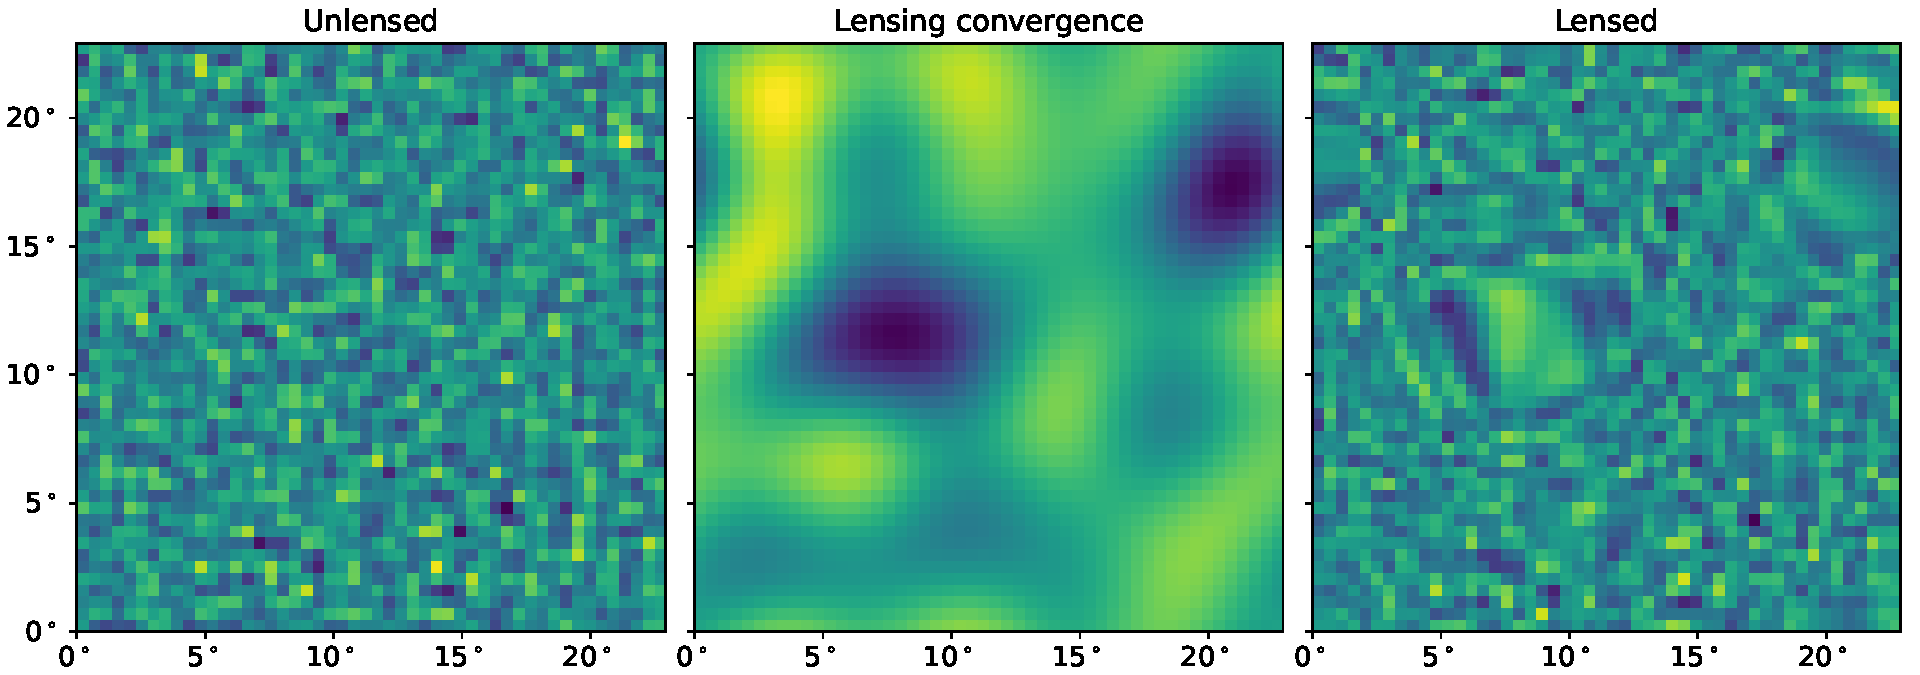
\includegraphics[width=\textwidth]{lensing_demo}
\caption{Demonstration of the CMB lensing process, where the convergence is exaggerated by a factor 30. The left panel shows the unlensed CMB field, the centre panel shows the convergence field (limited to $\lmax = 50$), and the right panel shows the lensed CMB field. Each panel covers a field of view of 22.9\,deg along each side.}
\label{ml_Fig:lensing_demo}
\end{figure}

For the early stages of this project (described in Sections \ref{ml_Sec:v1}--\ref{ml_Sec:v3}), lensing was exaggerated to simplify the problem. This was achieved by multiplying each convergence map by a constant factor (greater than 1) prior to simulating lensing. An example of the lensing process using a 30$\times$ exaggeration is shown in \autoref{ml_Fig:lensing_demo}. The left panel shows the unlensed CMB field, the centre panel shows the convergence field (limited to $\lmax = 50$), and the right panel shows the lensed CMB field. The lensing effect is clearly visible, which would not be the case without the 30$\times$ exaggeration.

\begin{figure}[tp]
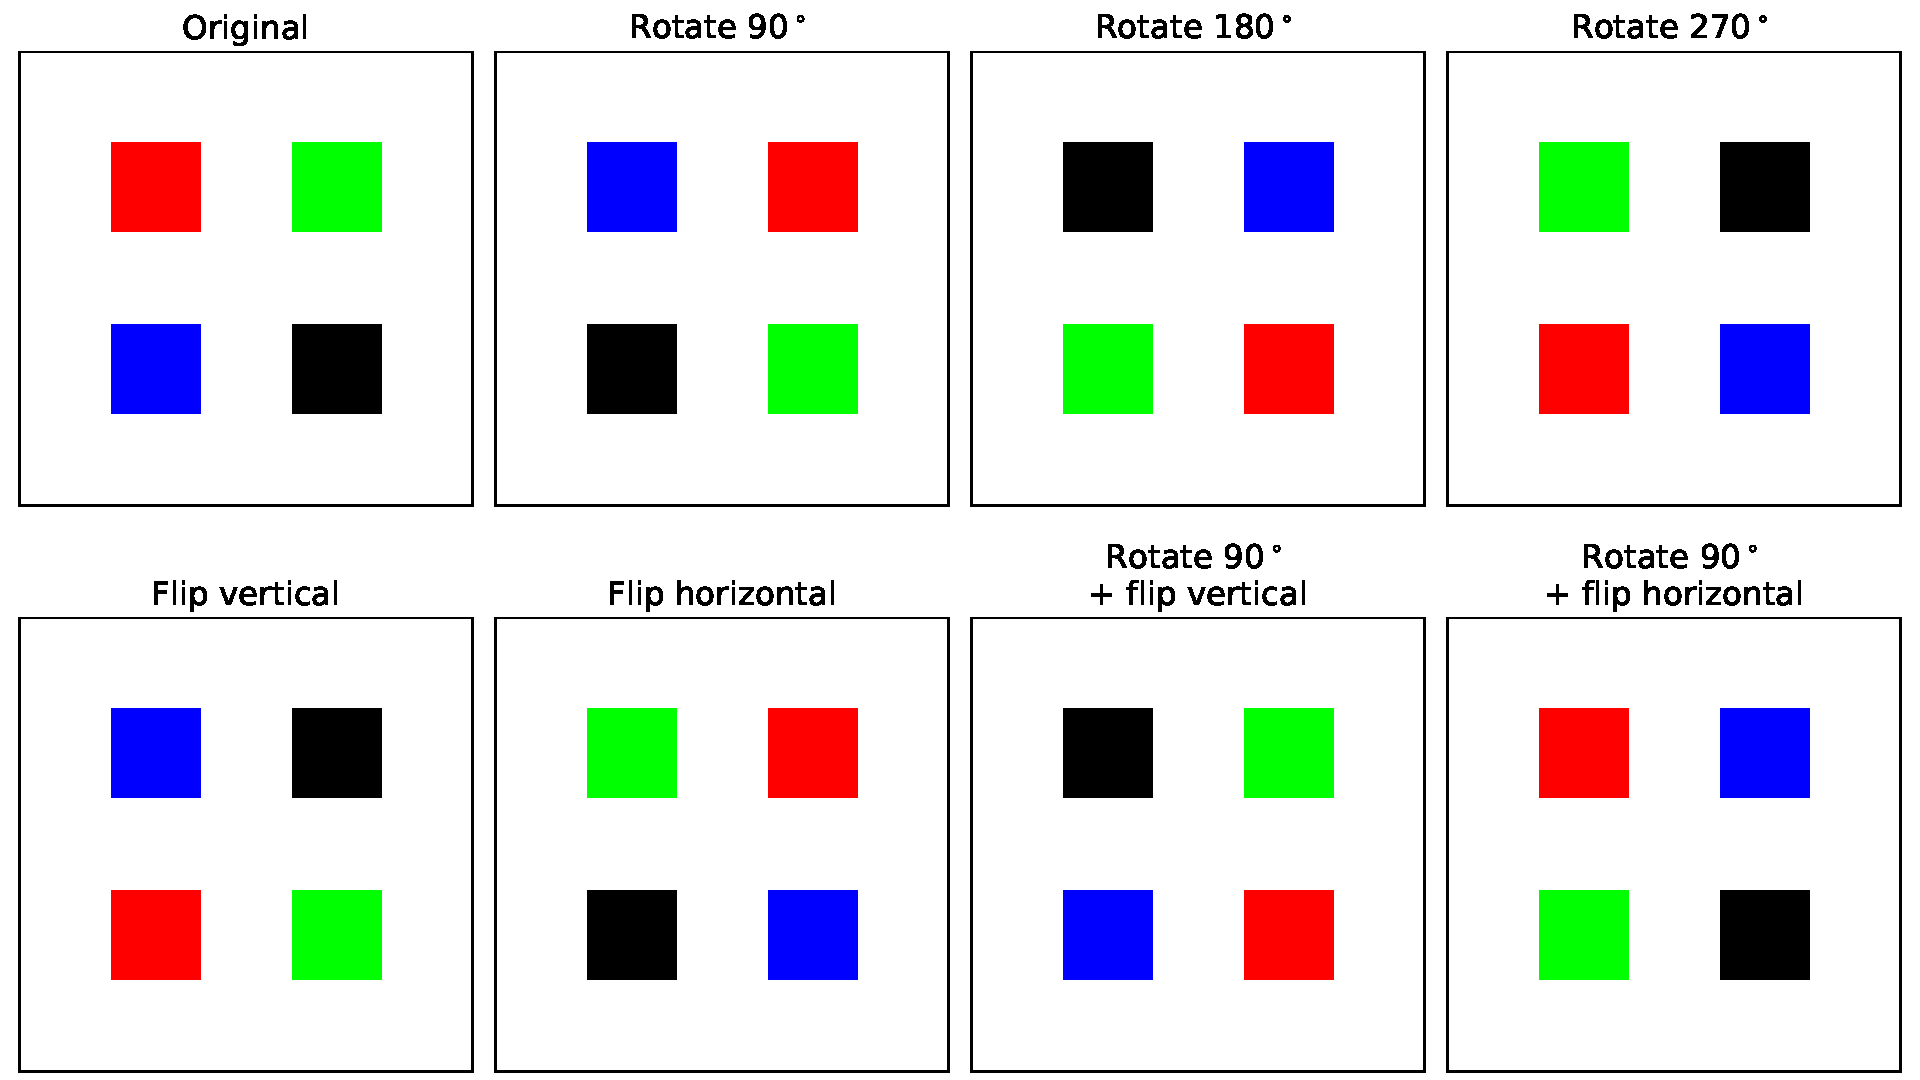
\includegraphics[width=\textwidth]{augmentation_demo}
\caption{Demonstration of the eight unique transforms used for data augmentation, each formed by a different combination of a rotation and a reflection (flip).}
\label{ml_Fig:augmentation_demo}
\end{figure}

From complexity level 2 onwards (described in Sections \ref{ml_Sec:v2}--\ref{ml_Sec:v6}), a method of data augmentation was used to multiply the size of the training set by a factor 8 without the need to simulate additional realisations. This also had the benefit of implicitly teaching the rotational invariance of lensing to the models during training. The augmentation method used eight unique combinations of rotations and reflections (flips). These were implemented using \texttt{NumPy} \citep{Harris2020} functions and are demonstrated in \autoref{ml_Fig:augmentation_demo}.

Training, validation and test data were always generated together and identically. Samples were shuffled prior to splitting into training, validation and test sets. Only the training set underwent data augmentation, after which it was re-shuffled prior to training, and again between each training epoch. All samples were scaled consistently to ensure that every pixel had a value between -1 and +1 while approximately maximising contrast within this range. This scaling was carried out independently for each complexity level.

\subsection{Model building and training}
\label{ml_Sec:model_building_training}

Convolutional neural networks were built, trained and tested using the open-source software \texttt{Keras}\footnote{\url{https://keras.io}} \citep{Chollet2015}. \texttt{Keras} is a Python deep learning API for \texttt{TensorFlow}\footnote{\url{https://www.tensorflow.org}} \citep{Abadi2016}, which is a powerful open-source machine learning library developed by Google. \texttt{TensorFlow} is optimised for the linear algebra operations that are inherent in neural network training. It is possible to develop neural networks directly in \texttt{TensorFlow} without using the \texttt{Keras} interface, but \texttt{Keras} greatly speeds up development by offering a simple yet highly customisable API.

The details of the neural network architectures used, and of the training process, are given in \autoref{ml_Sec:results}. These were developed and explored empirically using an iterative process of trial and error, bounded by the practical constraints of finite time and computing resources. Most of the time, it was possible to hold the entire training set in memory during training, even with the size of the training set being multiplied by 8 by the use of the data augmentation methods described in \autoref{ml_Sec:data_generation} above. However, for the final level of complexity explored in this chapter, which is described in \autoref{ml_Sec:v6}, the larger image size used (100$\times$100 pixels) meant this approach was no longer feasible. An alternative pipeline was therefore developed using a custom subclass of the \texttt{Sequence} object in \texttt{Keras}. The minimum functionality required of such a class is to provide a single batch of training data on request. In the default case, all batches would be loaded into memory on the initialisation of the object, and each would be supplied in turn on request. However, since this would take up too much memory in the case described here, the training set was not preloaded into memory, and instead each batch was loaded from disk only as it was requested, before being removed from memory when the subsequent batch was requested. This allowed the memory requirements to be significantly reduced when the volume of training data was large.

\section{Models explored and results with increasing complexity}
\label{ml_Sec:results}

As mentioned above, the structure of this project was to start with a relatively simple (and therefore unrealistic) problem, and gradually add complexity to converge towards a more realistic case. Six increasing levels of complexity are presented in this section, which are summarised below.
\begin{enumerate}
\item 22.9 degree field of view covered by 50 pixels along each side (equivalent HEALPix resolution: $N_\text{side} = 128$); CMB $\ell_\text{max} = 383$; convergence $\ell_\text{max} = 50$; convergence exaggerated by factor 30; same unlensed CMB realisation used throughout training, validation and testing.
\item As level 1, except a different CMB realisation used for each training, validation and test sample.
\item As level 2, but convergence exaggeration reduced to a factor 5.
\item As level 3, but no convergence exaggeration.
\item As level 4, except field of view reduced to 21.5 arcmin (equivalent HEALPix resolution: $N_\text{side} = 8192$); no CMB $\ell_\text{max}$ imposed; convergence $\ell_\text{max} = 24\,575$.
\item As level 4, except field of view reduced to 10 degrees and number of pixels along each side increased to 100 (approximate equivalent HEALPix resolution: $N_\text{side} \approx 512$); no $\ell_\text{max}$ imposed for CMB or convergence. (Note that while all other complexity levels are each based on the previous level, levels 5 and 6 are alternative progressions from level 4.)
\end{enumerate}

In the following subsections, each complexity level is described further, with a description of the different convolutional neural network architectures explored and the results obtained.

\subsection[Complexity level 1: Same CMB realisation, different lensing realisations~]{Complexity level 1: Same CMB realisation, different lensing realisations}
\label{ml_Sec:v1}

The investigation began with an extremely simple case of a single realisation of the CMB temperature field being lensed by many different convergence realisations. Each convergence field realisation was different for every training, validation, and test sample, but the unlensed CMB map used in each case was identical. The question was whether a CNN could learn the mapping from lensed CMB map to convergence map. To increase its chances, the lensing was strongly exaggerated by multiplying each convergence realisation by a factor 30 at the map level prior to applying the lensing transform, when generating the training data following the method described in \autoref{ml_Sec:data_generation}. A wide field covering a square of side 22.9 degrees was used, with a very low resolution of 50 pixels along each side. This was chosen to be equivalent in pixel area to a HEALPix \citep{Gorski2005} resolution of $N_\text{side} = 128$. The input CMB power spectrum was limited by the resolution of the map to a maximum multipole of $\ell_\text{max} = 383$, while the convergence power spectrum was truncated at $\ell_\text{max} = 50$ to further simplify the scenario.

Relatively few examples of image-to-image CNN models exist in the literature---excluding generative models, which are inappropriate for this problem as here we do not just require a generic realistic convergence map; we require the particular convergence map that corresponds to a specific lensed CMB map.\footnote{A notable exception is the DeepCMB model of \citet{Caldeira2019}, which has similar aims to this work, but we were not aware of that paper at the time.} One example of an image-to-image CNN model that appeared suitable as a starting point was the image super-resolution model described in \citet{Shi2016} and implemented as a \texttt{Keras} code example by \citet{Long2020}. The model is designed to be able to scale a previously unseen low-resolution image (or video) to higher resolution, using information it had learned from previously seeing many low- and high-resolution pairs of images in training. While this may seem distant from the problem at hand, it provides a valuable working example of an image-to-image CNN pipeline to use as a baseline. The model was first stripped of its super-resolution functionality, which was provided by a single convolutional layer with a low-resolution input and a higher-resolution output.

The remaining model used four convolutional layers: 64 nodes with a 5$\times$5 pixel kernel, 64 nodes with a 3$\times$3 kernel, 32 nodes with a 3$\times$3 kernel, and 1 final node with a 3$\times$3 kernel. All convolutions used a padding method (named \texttt{same} in \texttt{Keras}) whereby each image is padded with zeros prior to convolution such that the output from each layer has the same dimensions as the input. Each layer used orthogonal initialisation and a ReLU activation function (see \autoref{ml_Sec:cnns}). All other options in the model followed the \texttt{Keras} defaults: single-stride convolution was used, with a bias vector initialised as zeros; no regulariser was applied to any kernel, bias vector, or output, nor was a constraint function applied to any kernel or bias vector.

For training, the Adam optimiser was used (see \autoref{ml_Sec:cnns}) with the default parameters of a learning rate of $\alpha = 10^{-3}$, exponential decay rates of $\beta_1 = 0.9$ and $\beta_2 = 0.999$ and numerical stability constant $\epsilon = 10^{-7}$. The AMSGrad variation of the Adam algorithm introduced in \citet{Reddi2018}, which may assist convergence in some cases, was not used. A mean squared error loss function was used (\autoref{ml_Eqn:mse}).

\begin{figure}[tp]
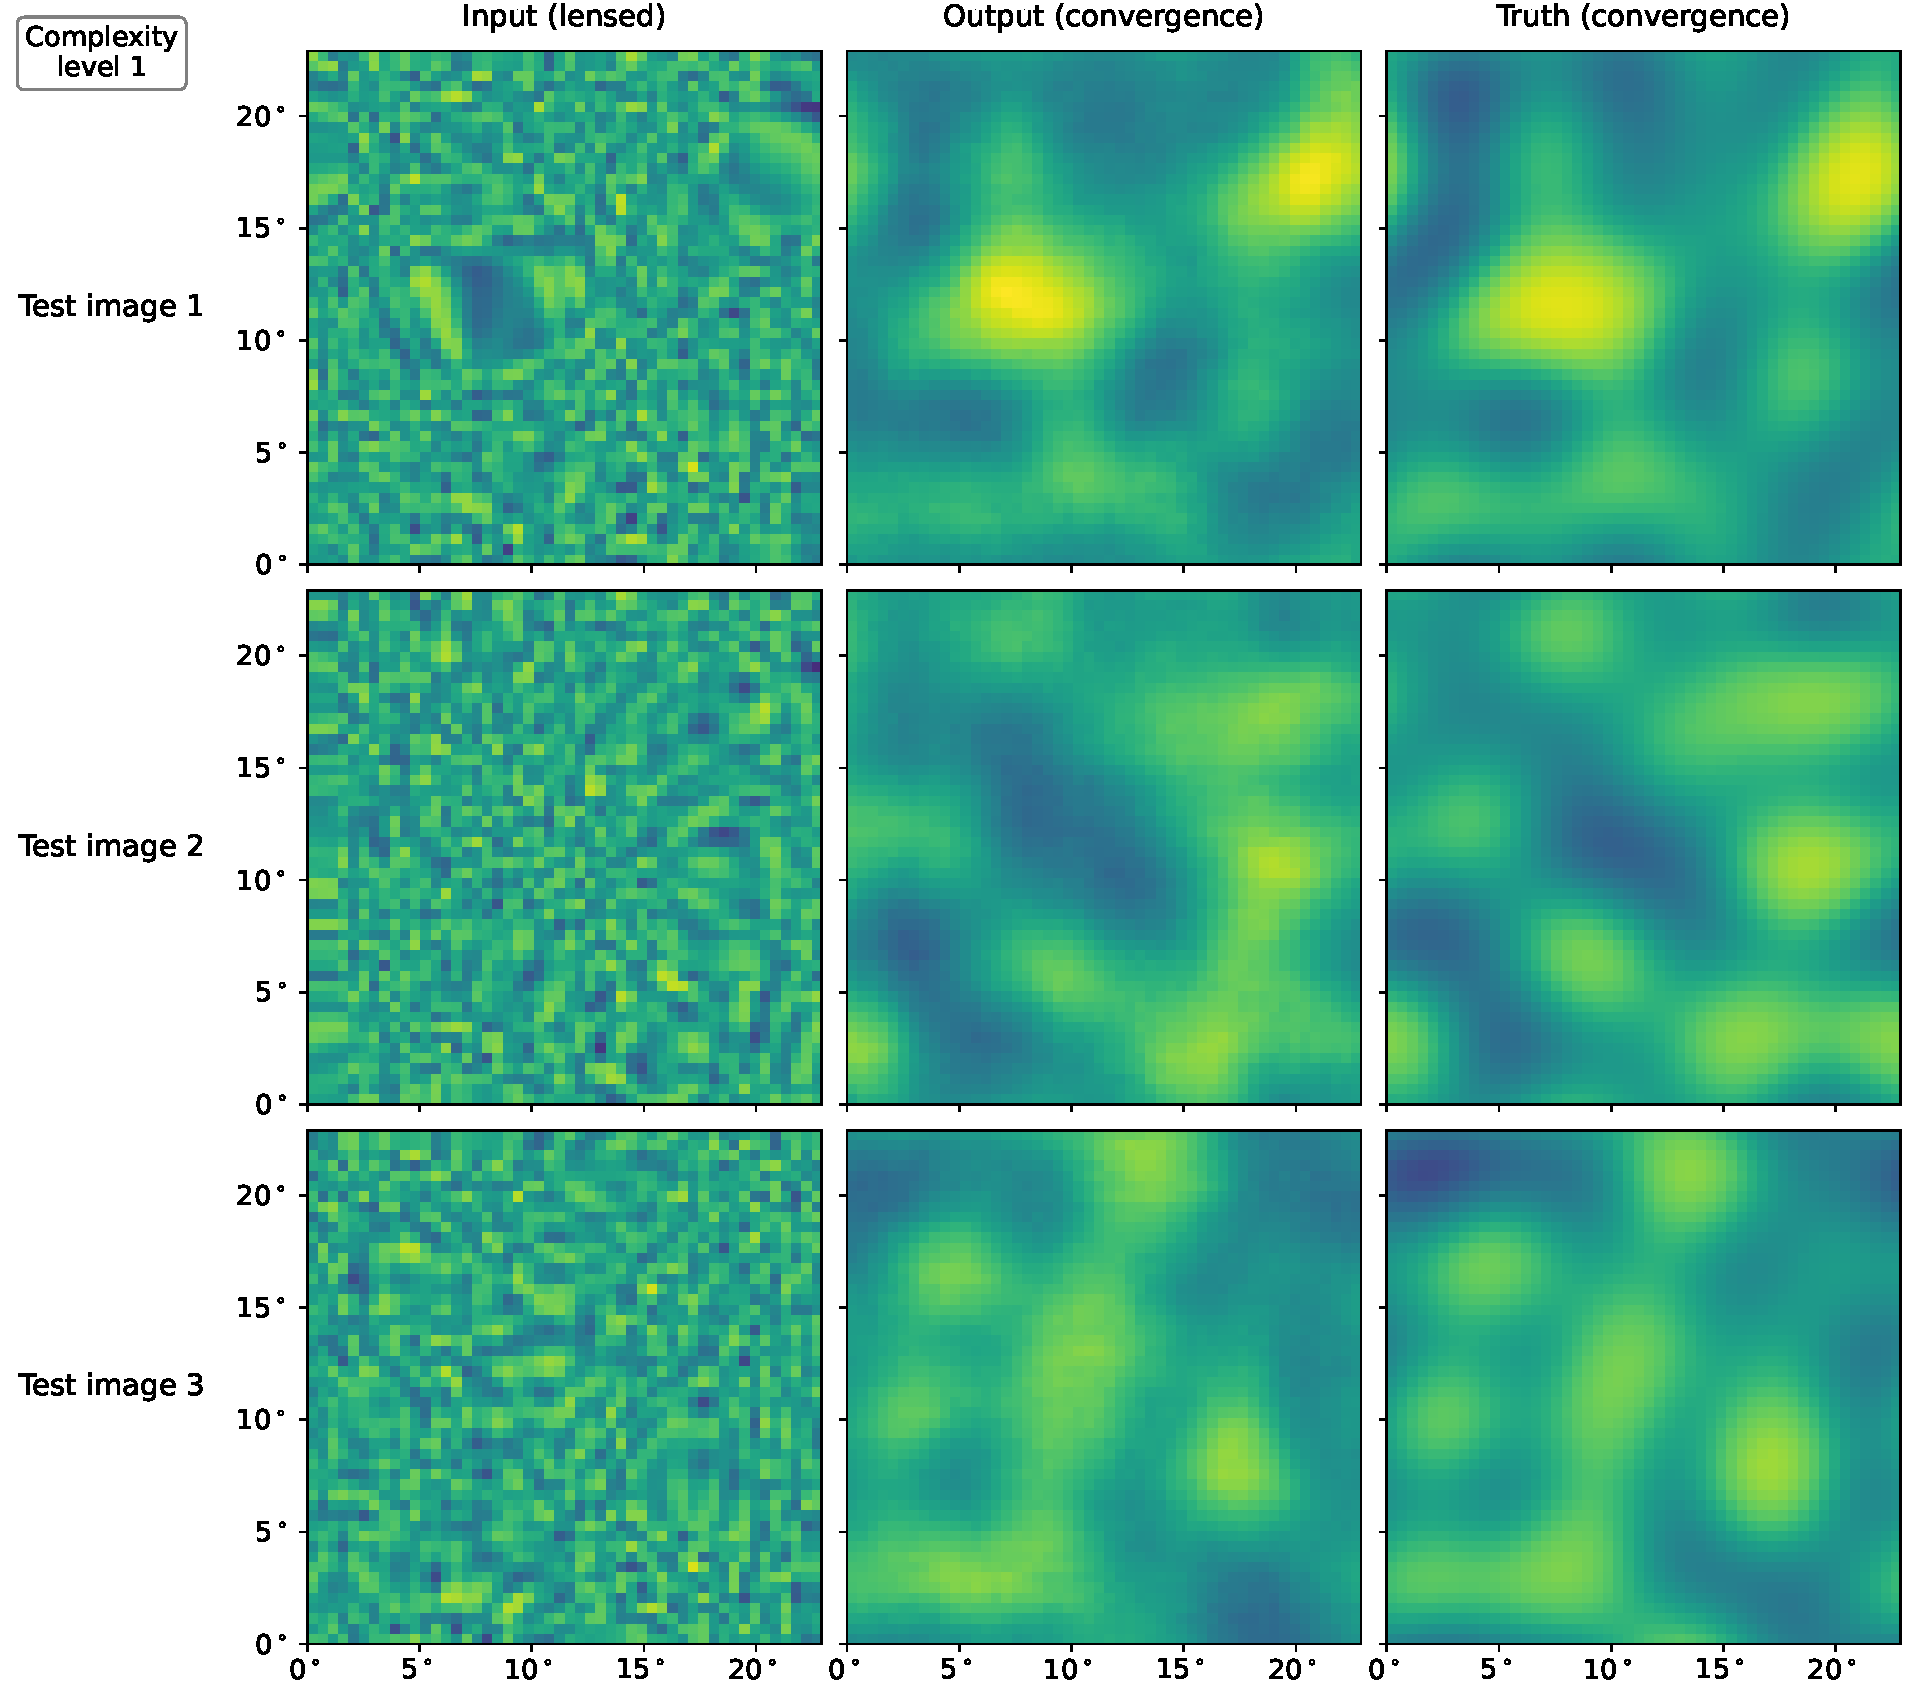
\includegraphics[width=\textwidth]{v1_3x3}
\caption{Performance of the best-performing model for complexity level 1 (described in \autoref{ml_Sec:v1}) on three previously unseen test images. Rows correspond to the different test images, while the columns show, from left to right: the lensed CMB map given as input to the model, the predicted convergence map produced by the model, and the true convergence map that was used to generate the test image in the first column. The model was trained for 50 epochs on a training set of 800 samples, with a validation set of 200 samples.}
\label{ml_Fig:v1_3x3}
\end{figure}

Many variations from this baseline model were explored. Each was trained for 5 epochs with a training set of 800 samples and a batch size of 32, and validated once per epoch with a separate validation set of 200 samples, and finally evaluated against an unseen test set of 3 samples. Evaluation was primarily a visual comparison to the true convergence field for each test sample (an example may be seen for the best-performing model in \autoref{ml_Fig:v1_3x3}, which is described below). The variations explored were as follows:
\begin{itemize}
\item Changing the kernel initialisation from orthogonal to the Glorot uniform initialiser \citep{Glorot2010}, which is the \texttt{Keras} default for a convolutional layer. This draws the initial value for each kernel pixel $W$ independently from a uniform distribution as
\begin{equation}
W \sim U \left( - W_\text{max},~ W_\text{max} \right),
\end{equation}
with
\begin{equation}
W_\text{max} = \sqrt{\frac{6}{n_j + n_{j + 1}}},
\end{equation}
where $n_j$ is the number of nodes in layer $j$. However, the performance with this method was slightly worse compared to orthogonal initialisation.
\item Varying the kernel size in the final layer: sizes of 3$\times$3, 5$\times$5, 7$\times$7, 9$\times$9 and 11$\times$11 pixels were explored, with performance peaking at 9$\times$9 for this particular low-resolution setup.
\item Varying the kernel size in the other layers: a small kernel of size 3$\times$3 was found to be optimal.
\item Adding additional layers: many combinations of number of nodes and kernel size were explored, from 2 nodes to 64 and from 3$\times$3 to 7$\times$7, but each one degraded performance compared to the baseline model.
\item Removing layers, but removing any layer was found to degrade the performance of the model.
\item Increasing the number of nodes in the first layer from 64 to 128, which also degraded the performance, so increasing the numbers of nodes in other layers was not explored.
\end{itemize}

The conclusion from all of this testing was that the best-performing model over 5 epochs was only a very small variation on the initial model taken from the image super-resolution problem: four convolutional layers comprising 64 nodes with a 3$\times$3 kernel, another 64 nodes with a 3$\times$3 kernel, 32 nodes with a 3$\times$3 kernel, and 1 final node with a 9$\times$9 kernel. This model was then trained for 50 epochs using the same training and validation sets as described above (800 training samples and 200 validation samples), reaching a minimum validation loss on epoch of 45 of $\mathcal{L}_\text{val} = 2.1 \times 10^3$.\footnote{Quoted loss values cannot be compared between different complexity levels, because each level uses its own scaling of the training, validation and test samples to ensure that all inputs to the CNN are in the range (-1, 1) while approximately maximising the contrast within this range, as discussed in \autoref{ml_Sec:data_generation}.} The model was then applied to an unseen test set of three samples, which are shown in \autoref{ml_Fig:v1_3x3}. The three rows correspond to the three different test images, while the columns show, from left to right: the lensed CMB map given as input to the model, the predicted convergence map produced by the model, and the true convergence map that was used to generate the test image in the first column. Visually the performance is very good, with a clear correspondence between the estimate and the truth for all three test samples.

\subsection{Complexity level 2: Different CMB realisations}
\label{ml_Sec:v2}

The second level of complexity was to no longer use the same unlensed CMB realisation across all samples; instead, a different realisation (from the same underlying power spectrum) was used for every sample in the training, validation and test sets. All other aspects were identical to complexity level 1 described in \autoref{ml_Sec:v1} above, including that each convergence field was exaggerated by a factor 30.

The baseline model for this level was a small variation on the best model from the previous level. Early testing prior to implementing data augmentation (described below) yielded a better performance with 64 nodes on the third layer as well as the first two, giving a baseline model comprising four convolutional layers: three of 64 nodes with a 3$\times$3 kernel followed by 1 final node with a 9$\times$9 kernel. All other aspects of the model, optimiser and loss function used were identical to complexity level 1. This model will be referred to as \texttt{L2\_baseline}.

For this complexity level, data augmentation was introduced to multiply the size of the training set by a factor 8, as described in \autoref{ml_Sec:data_generation}, as well as to implicitly teach the rotational invariance of lensing to the model. Prior to augmentation, the training set contained 800 samples and the validation set contained 200 samples. Augmentation was applied to the training set to give 6400 training samples. The validation set was not augmented to avoid any possible bias.

\begin{figure}[p]%[tp]
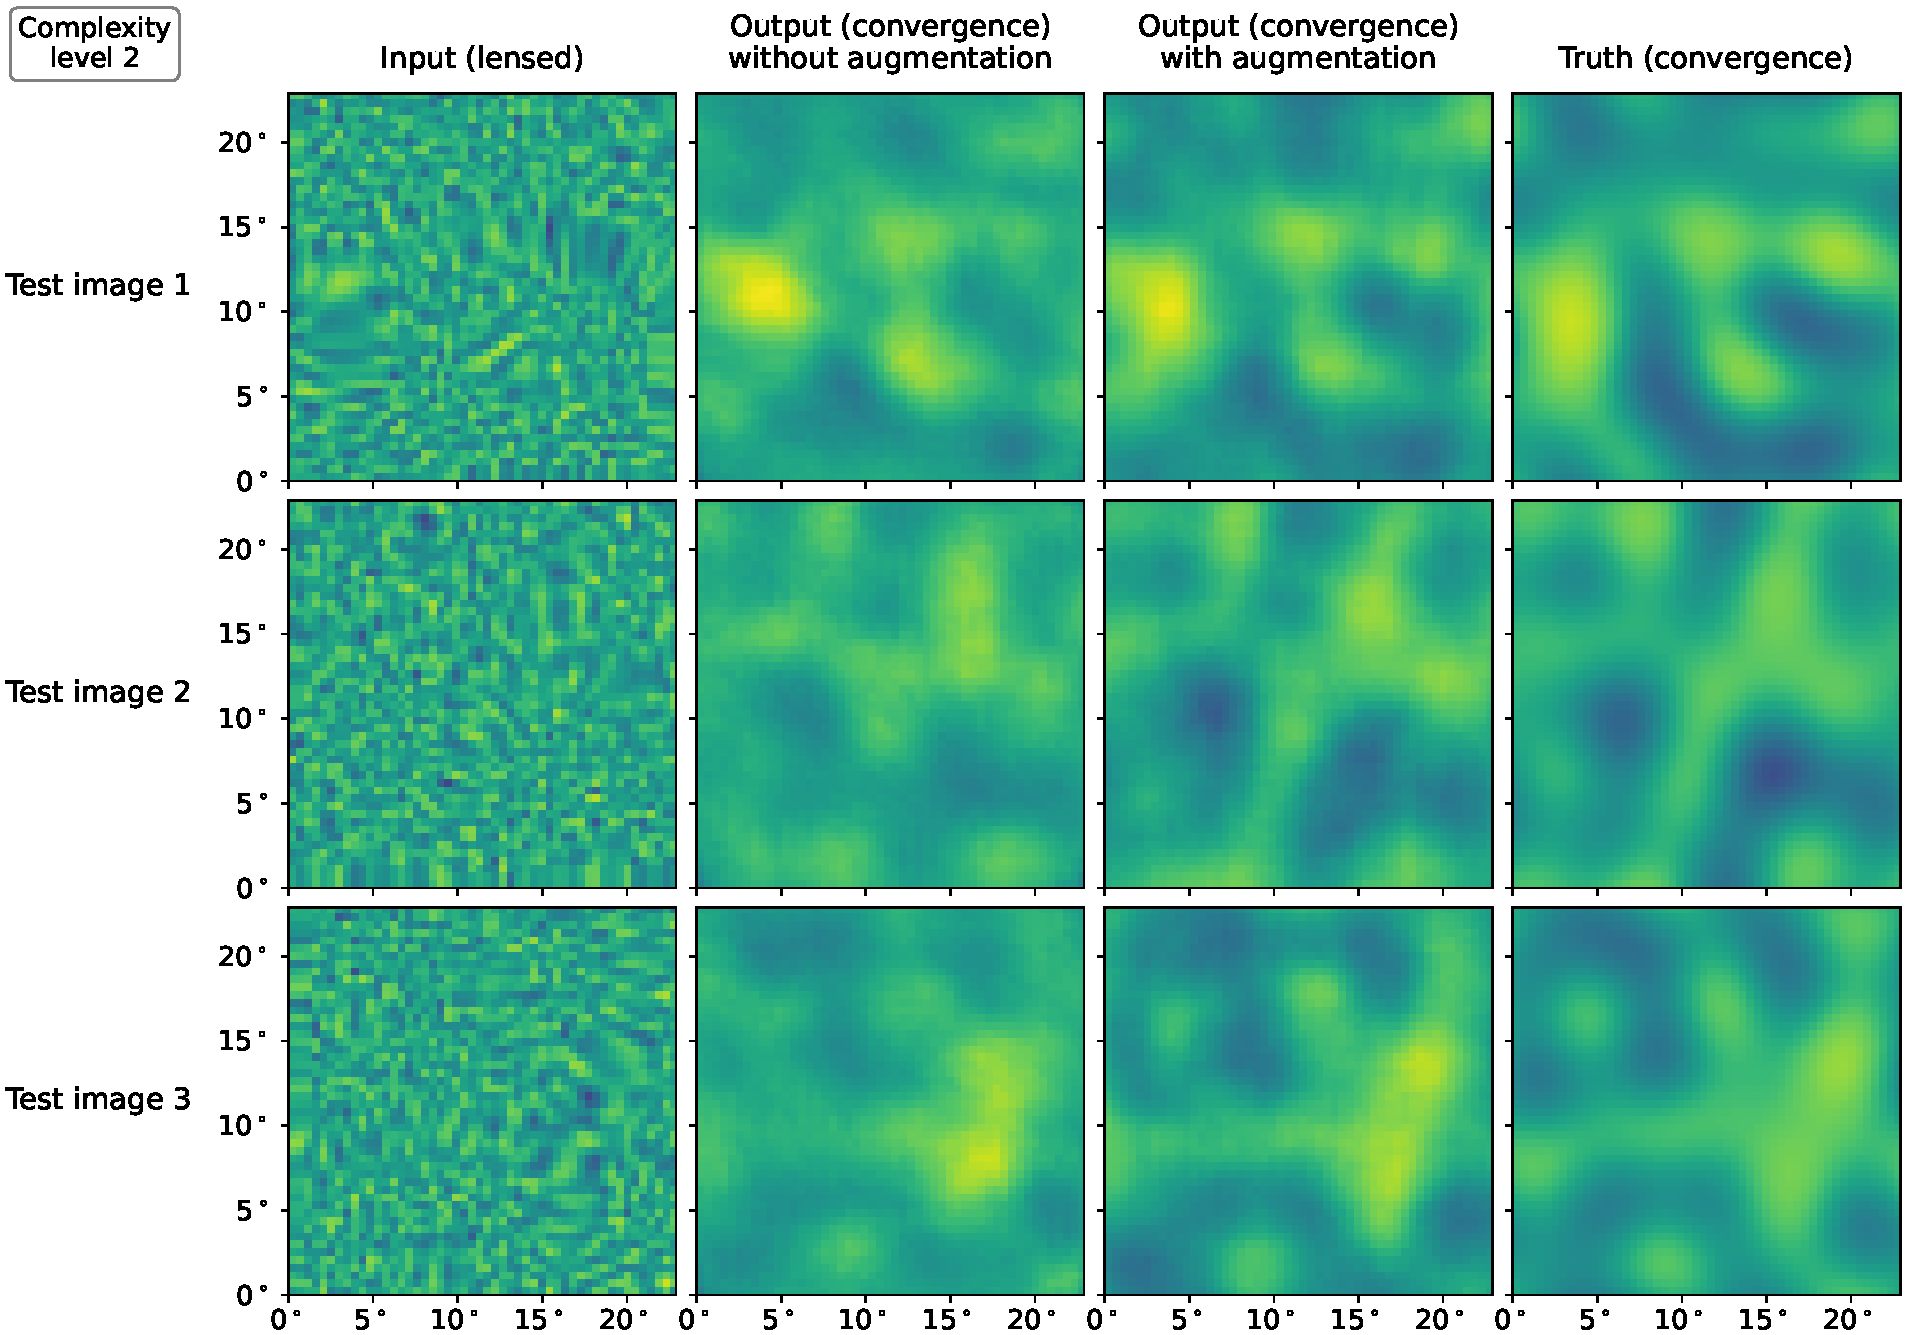
\includegraphics[width=\textwidth]{v2augtest_3x4}
\caption{The effect of data augmentation on the performance of the \texttt{L2\_baseline} model, evaluated on three previously unseen test samples after having been trained for 10 epochs on the same training set with and without data augmentation.
Rows correspond to the different test images, while the columns show, from left to right: the lensed CMB map given as input to the model, the predicted convergence map produced by the model after training without data augmentation, the predicted convergence map after training with data augmentation, and the true convergence map that was used to generate the test image in the first column. The training set contained 800 samples prior to augmentation, with a validation set of 200 samples which was not augmented.}
\label{ml_Fig:v2augtest_3x4}
\end{figure}

\begin{figure}[p]%[tp]
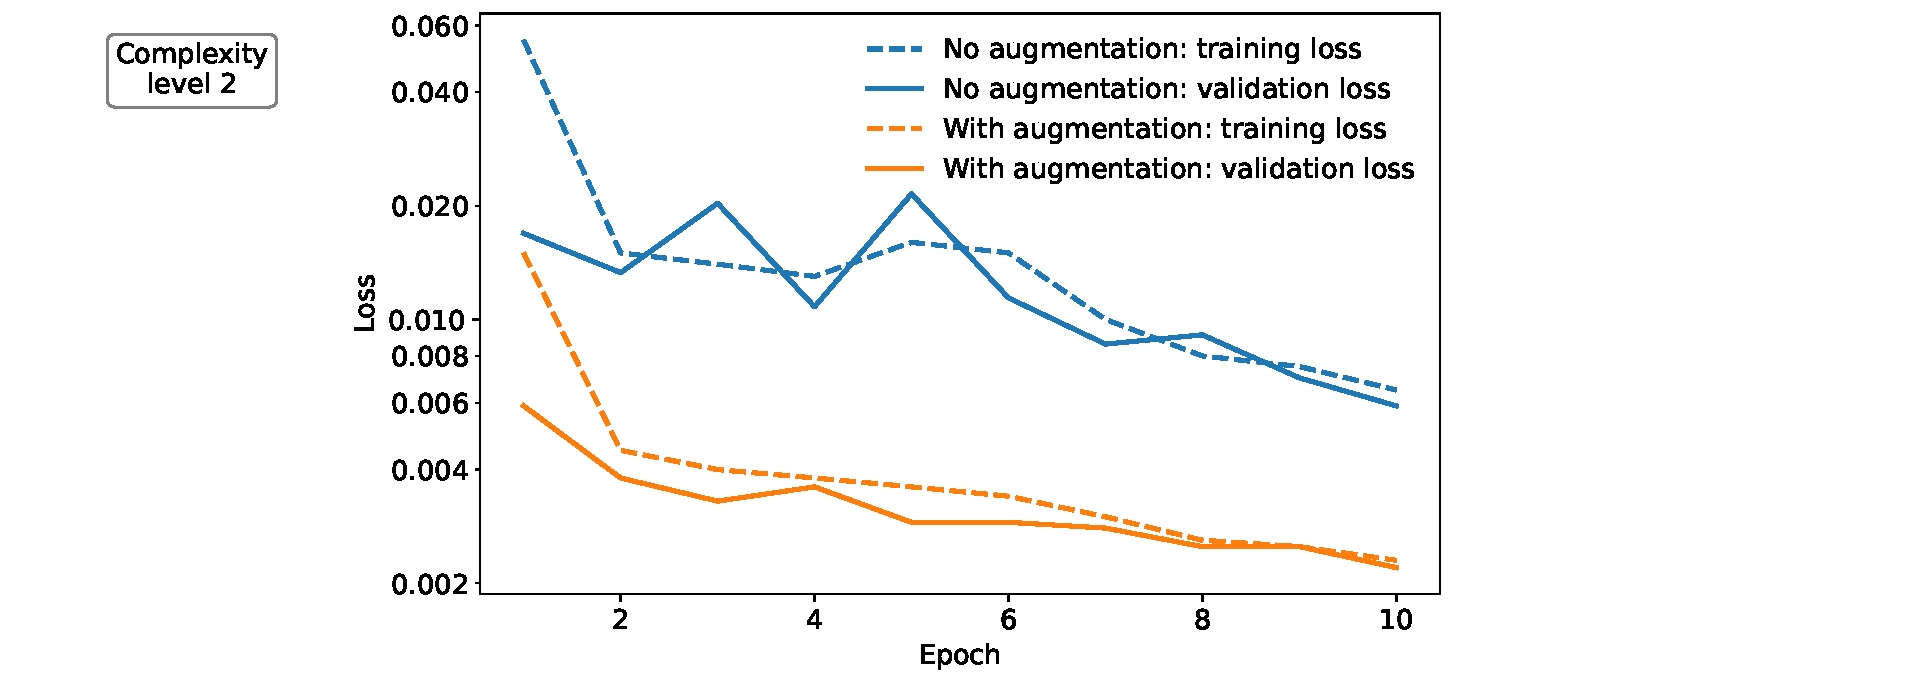
\includegraphics[width=\textwidth]{v2augtest_loss}
\caption{Training and validation loss for the \texttt{L2\_baseline} model over 10 epochs with and without data augmentation. The training set contained 800 samples prior to augmentation, with a validation set of 200 samples which was not augmented.}
\label{ml_Fig:v2augtest_loss}
\end{figure}

Data augmentation turned out to be highly effective in increasing the performance of the model over a given number of epochs. \autoref{ml_Fig:v2augtest_3x4} shows the \texttt{L2\_baseline} model evaluated on an unseen test set (which was not augmented) after having been trained for 10 epochs on the same training set with and without data augmentation. There is clearly a closer resemblance to the true convergence field in the augmented case. This is also illustrated by the training and validation loss per training epoch in each case, which is shown in \autoref{ml_Fig:v2augtest_loss}. There is a consistent factor 2.5--5 improvement in both loss values throughout training, reaching respective minima of $\mathcal{L}_\text{val} = 5.9 \times 10^3$ without augmentation and $\mathcal{L}_\text{val} = 2.2 \times 10^3$ with augmentation.

With data augmentation in place, three variations on the baseline model were explored, which are summarised along with the baseline model as follows:
\begin{itemize}
\item \texttt{L2\_baseline}: \\
% \hspace*{1em}--~64 nodes with a 3$\times$3 kernel; \\
% \hspace*{1em}--~64 nodes with a 3$\times$3 kernel; \\
% \hspace*{1em}--~64 nodes with a 3$\times$3 kernel; \\
% \hspace*{1em}--~1 node with a 9$\times$9 kernel.
\hspace*{1em}Layers 1--3:~64 nodes with a 3$\times$3 kernel; \\
% \hspace*{1em}--~64 nodes with a 3$\times$3 kernel; \\
% \hspace*{1em}--~64 nodes with a 3$\times$3 kernel; \\
\hspace*{1em}Layer 4:~~~~~~1 node with a 9$\times$9 kernel.
\item \texttt{L2\_+32}: \\
\hspace*{1em}As \texttt{L2\_baseline}, but with an additional layer containing 32 nodes with a 3$\times$3 kernel before the final layer.
\item \texttt{L2\_+64}: \\
\hspace*{1em}As \texttt{L2\_baseline}, but with an additional layer containing 64 nodes with a 3$\times$3 kernel before the final layer.
\item \texttt{L2\_first-layer-128}: \\
\hspace*{1em}As \texttt{L2\_baseline}, but with the first layer having 128 nodes instead of 64.
\end{itemize}

\begin{figure}[tp]
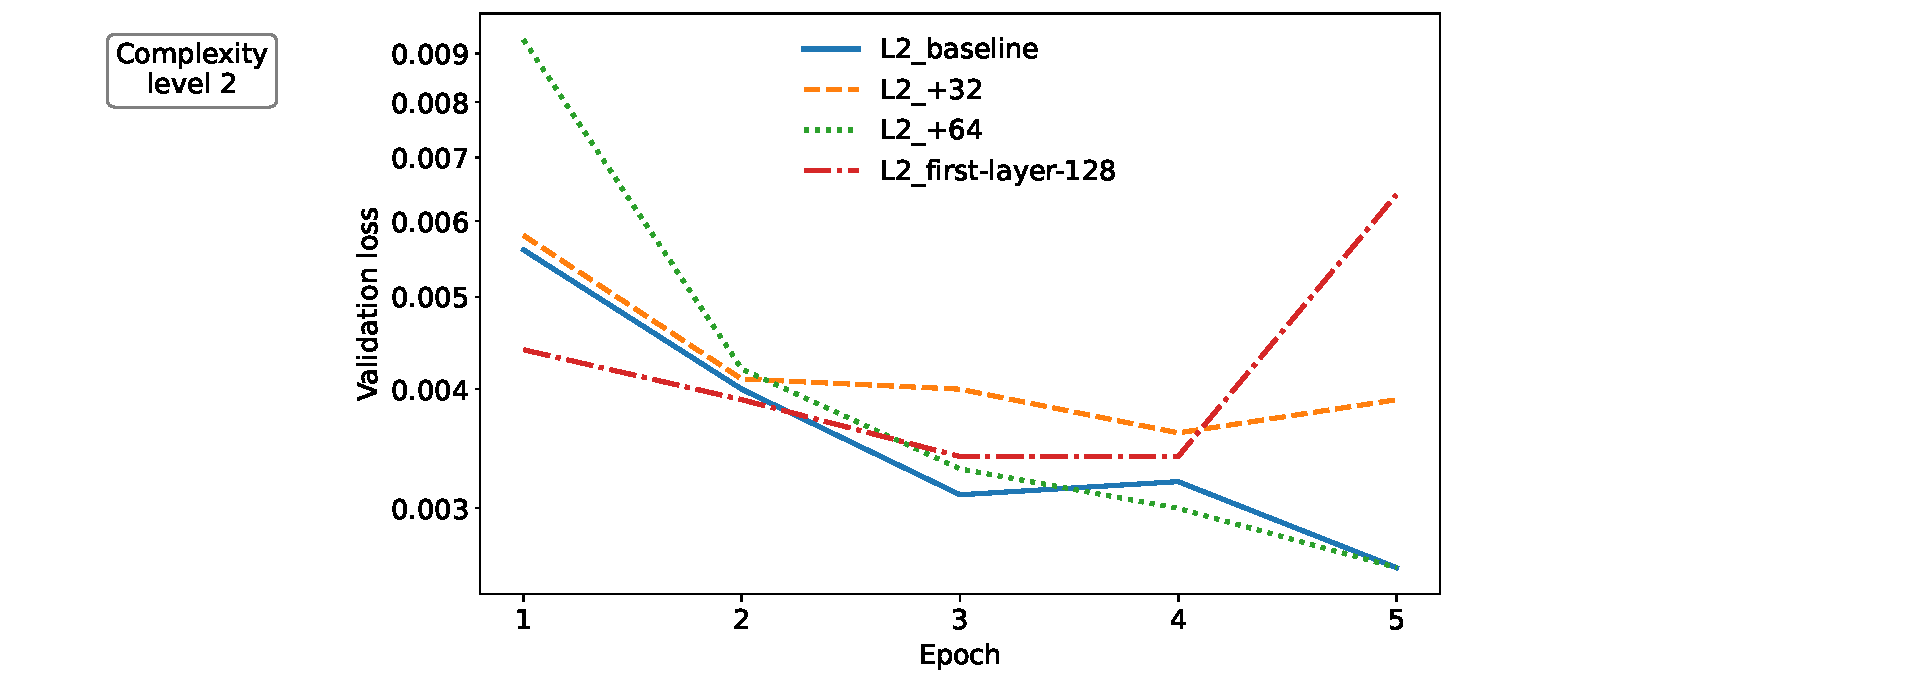
\includegraphics[width=\textwidth]{v2_loss}
\caption{Validation loss compared between the four models explored in complexity level 2, which are described in \autoref{ml_Sec:v2}. Each model was trained for 5 epochs on the same training set containing 800 samples prior to augmentation by a factor 8, and validated on 200 different samples which were not augmented.}
\label{ml_Fig:v2_loss}
\end{figure}

\begin{figure}[tp]
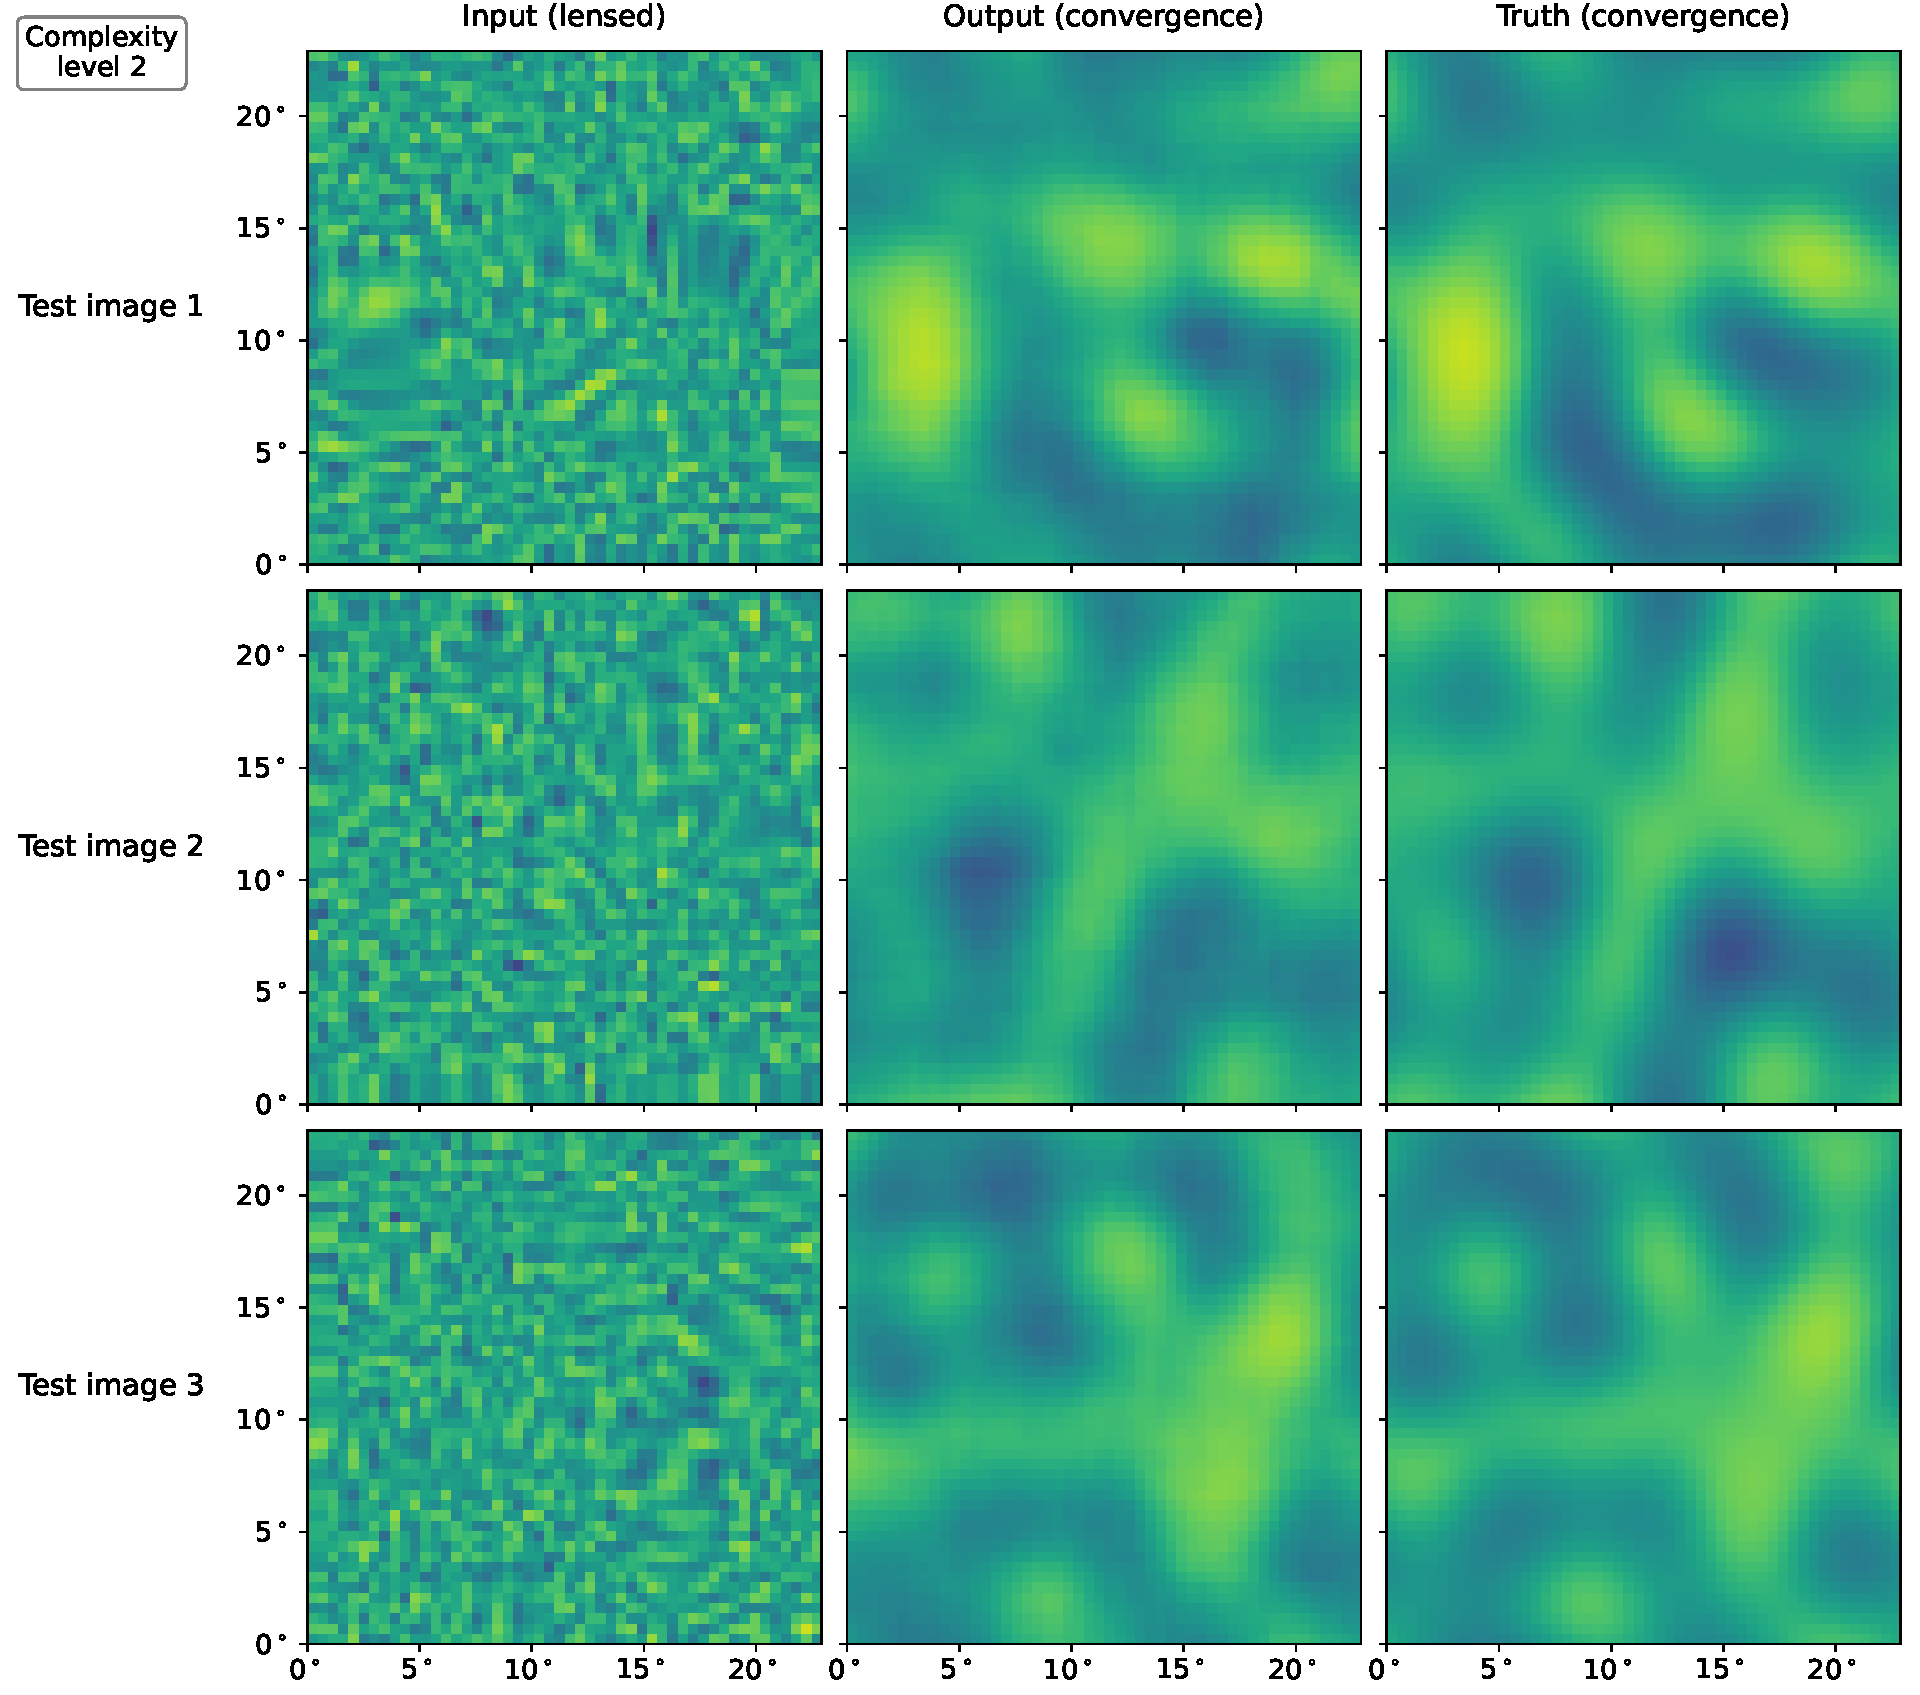
\includegraphics[width=\textwidth]{v2_3x3}
\caption{Performance of the best-performing \texttt{L2\_+64} model for complexity level 2 (described in \autoref{ml_Sec:v1}) on three previously unseen test images. Rows correspond to the different test images, while the columns show, from left to right: the lensed CMB map given as input to the model, the predicted convergence map produced by the model, and the true convergence map that was used to generate the test image in the first column. The model was trained for 50 epochs on a training set of 800 samples augmented by a factor 8, with a validation set of 200 samples which was not augmented.}
\label{ml_Fig:v2_3x3}
\end{figure}

Each model was trained for 5 epochs on the same training set, containing 800 samples prior to augmentation, which increased the number of samples by a factor 8. A validation set containing 200 samples was again used, and not augmented. Each model was evaluated based on its visual performance on a test set of 3 previously unseen images, and on its validation loss during training. These two measures were consistently in agreement. \autoref{ml_Fig:v2_loss} shows the validation loss of each model over the training period. The best-performing models were the \texttt{L2\_baseline} and \texttt{L2\_+64} models, which both ended epoch 5 with an identical validation loss of $\mathcal{L}_\text{val} = 2.6 \times 10^{-3}$.

The \texttt{L2\_+64} model was re-trained for 10 epochs to obtain a comparison with the \texttt{L2\_} \texttt{baseline} model, which was previously trained for 10 epochs when testing the effect of data augmentation as described above. This revealed a visual performance on the test set that slightly surpassed that of the baseline model, with a validation loss of $\mathcal{L}_\text{val} = 1.8 \times 10^{-3}$ (compared to the corresponding 10-epoch value obtained above for the \texttt{L2\_baseline} model of $\mathcal{L}_\text{val} = 2.2 \times 10^{-3}$). The \texttt{L2\_+64} model was therefore selected to train for 50 epochs on the same training set, reaching a best validation loss of $\mathcal{L}_\text{val} = 1.13 \times 10^{-3}$ in epoch 50. The predictions made by this model on the previously unseen test set are shown in \autoref{ml_Fig:v2_3x3}. Visually the performance is good, roughly comparable with those from complexity level 1 (\autoref{ml_Fig:v1_3x3}) despite using a different unlensed CMB realisation for each sample.

\subsection{Complexity level 3: Reduced lensing exaggeration}
\label{ml_Sec:v3}

The third level of complexity was to reduce the exaggeration of the convergence field to a factor 5, from the value of 30 used in levels 1 and 2. All other aspects of the setup were identical to level 2, i.e. a different unlensed CMB realisation was used for each sample and the resolution settings were the same as described for level 1 in \autoref{ml_Sec:v1}.

The exaggeration factor of 5 was chosen as the result of some initial exploratory testing, carried out over 5 epochs with a training set containing 800 samples, augmented by a factor 8, and a validation set of 200 samples, which was not augmented. These tests used the best-performing \texttt{L2\_+64} model from complexity level 2 (described in \autoref{ml_Sec:v2} above) as the new baseline model, here renamed \texttt{L3\_baseline}. This initial testing found that disabling lensing exaggeration entirely yielded a completely blank prediction of the convergence field for all test samples, and a validation loss that immediately plateaued at $\mathcal{L}_\text{val} = 1.4 \times 10^{-2}$. This would be a difficult starting point, since a working baseline is effectively an essential requirement for finding iterative improvements. An exaggeration factor of 10 was also explored, but this performed comparably well to a factor of 30, reaching a 5-epoch validation loss of $\mathcal{L}_\text{val} = 2.8 \times 10^{-3}$, compared to $\mathcal{L}_\text{val} = 2.0 \times 10^{-3}$ for an equivalent run with data from complexity level 2 (using an equivalent scaling, therefore allowing for a valid comparison). An exaggeration factor of 5 was ultimately chosen as it produced a relatively poor performance ($\mathcal{L}_\text{val} = 8.2 \times 10^{-3}$) in the \texttt{L3\_baseline} model over 5 epochs, while still producing a validation loss that was steadily decreasing and being able to predict some features in the true convergence maps of the test sample. This made it a suitable starting point for improvements, with an aim towards removing the lensing exaggeration altogether in the next complexity level (\autoref{ml_Sec:v4}).

\begin{figure}[tp]
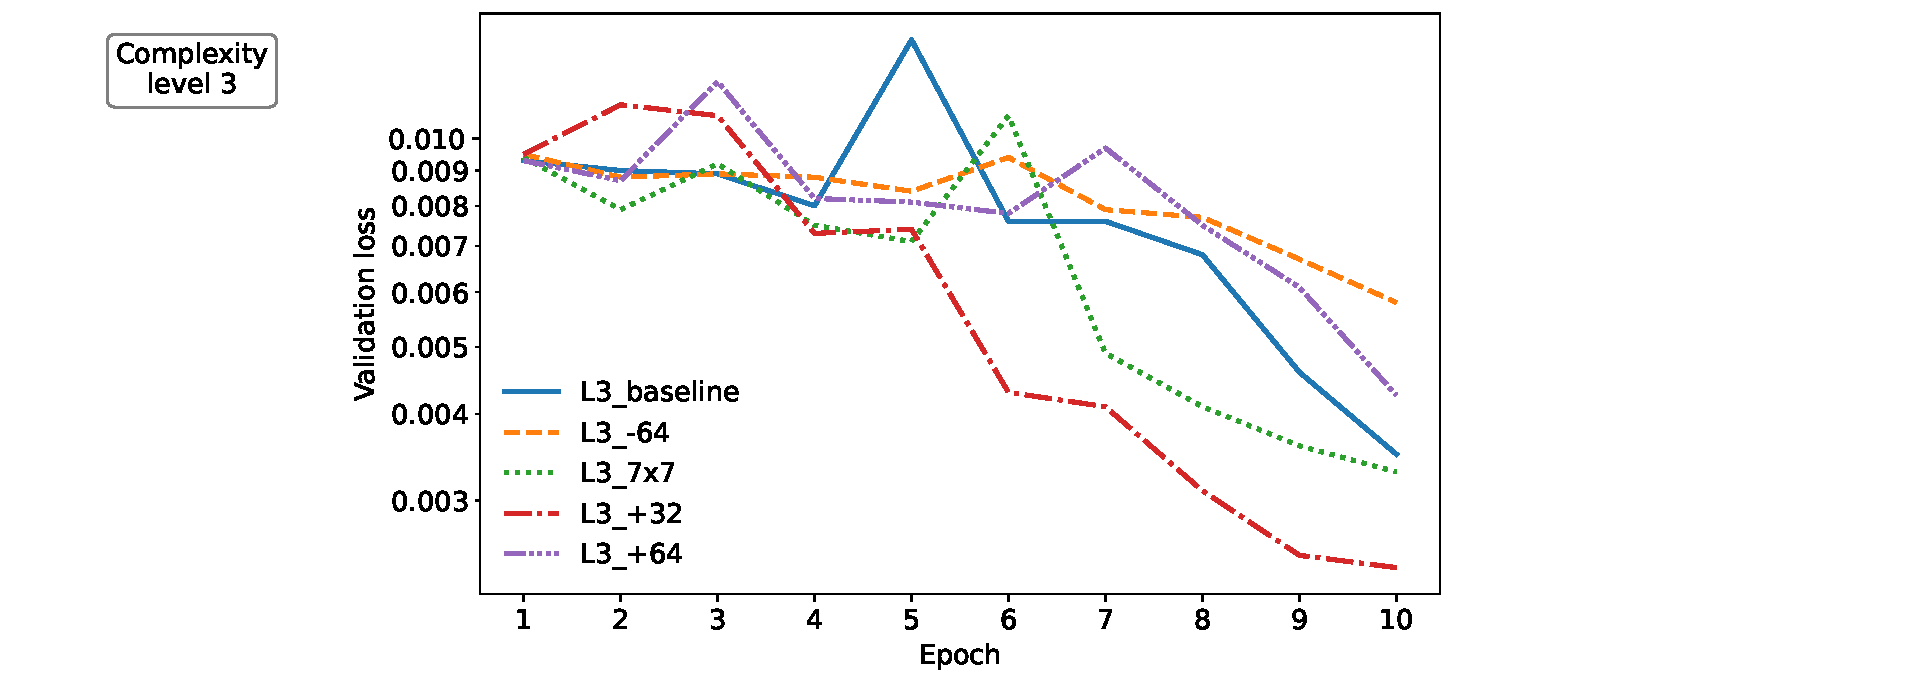
\includegraphics[width=\textwidth]{v3_loss}
\caption{Validation loss compared between the five best-performing models explored in complexity level 3, which are described in \autoref{ml_Sec:v3}. Each model was trained for 10 epochs on the same training set containing 800 samples prior to augmentation by a factor 8, and validated on 200 different samples which were not augmented.}
\label{ml_Fig:v3_loss}
\end{figure}

\begin{figure}[tp]
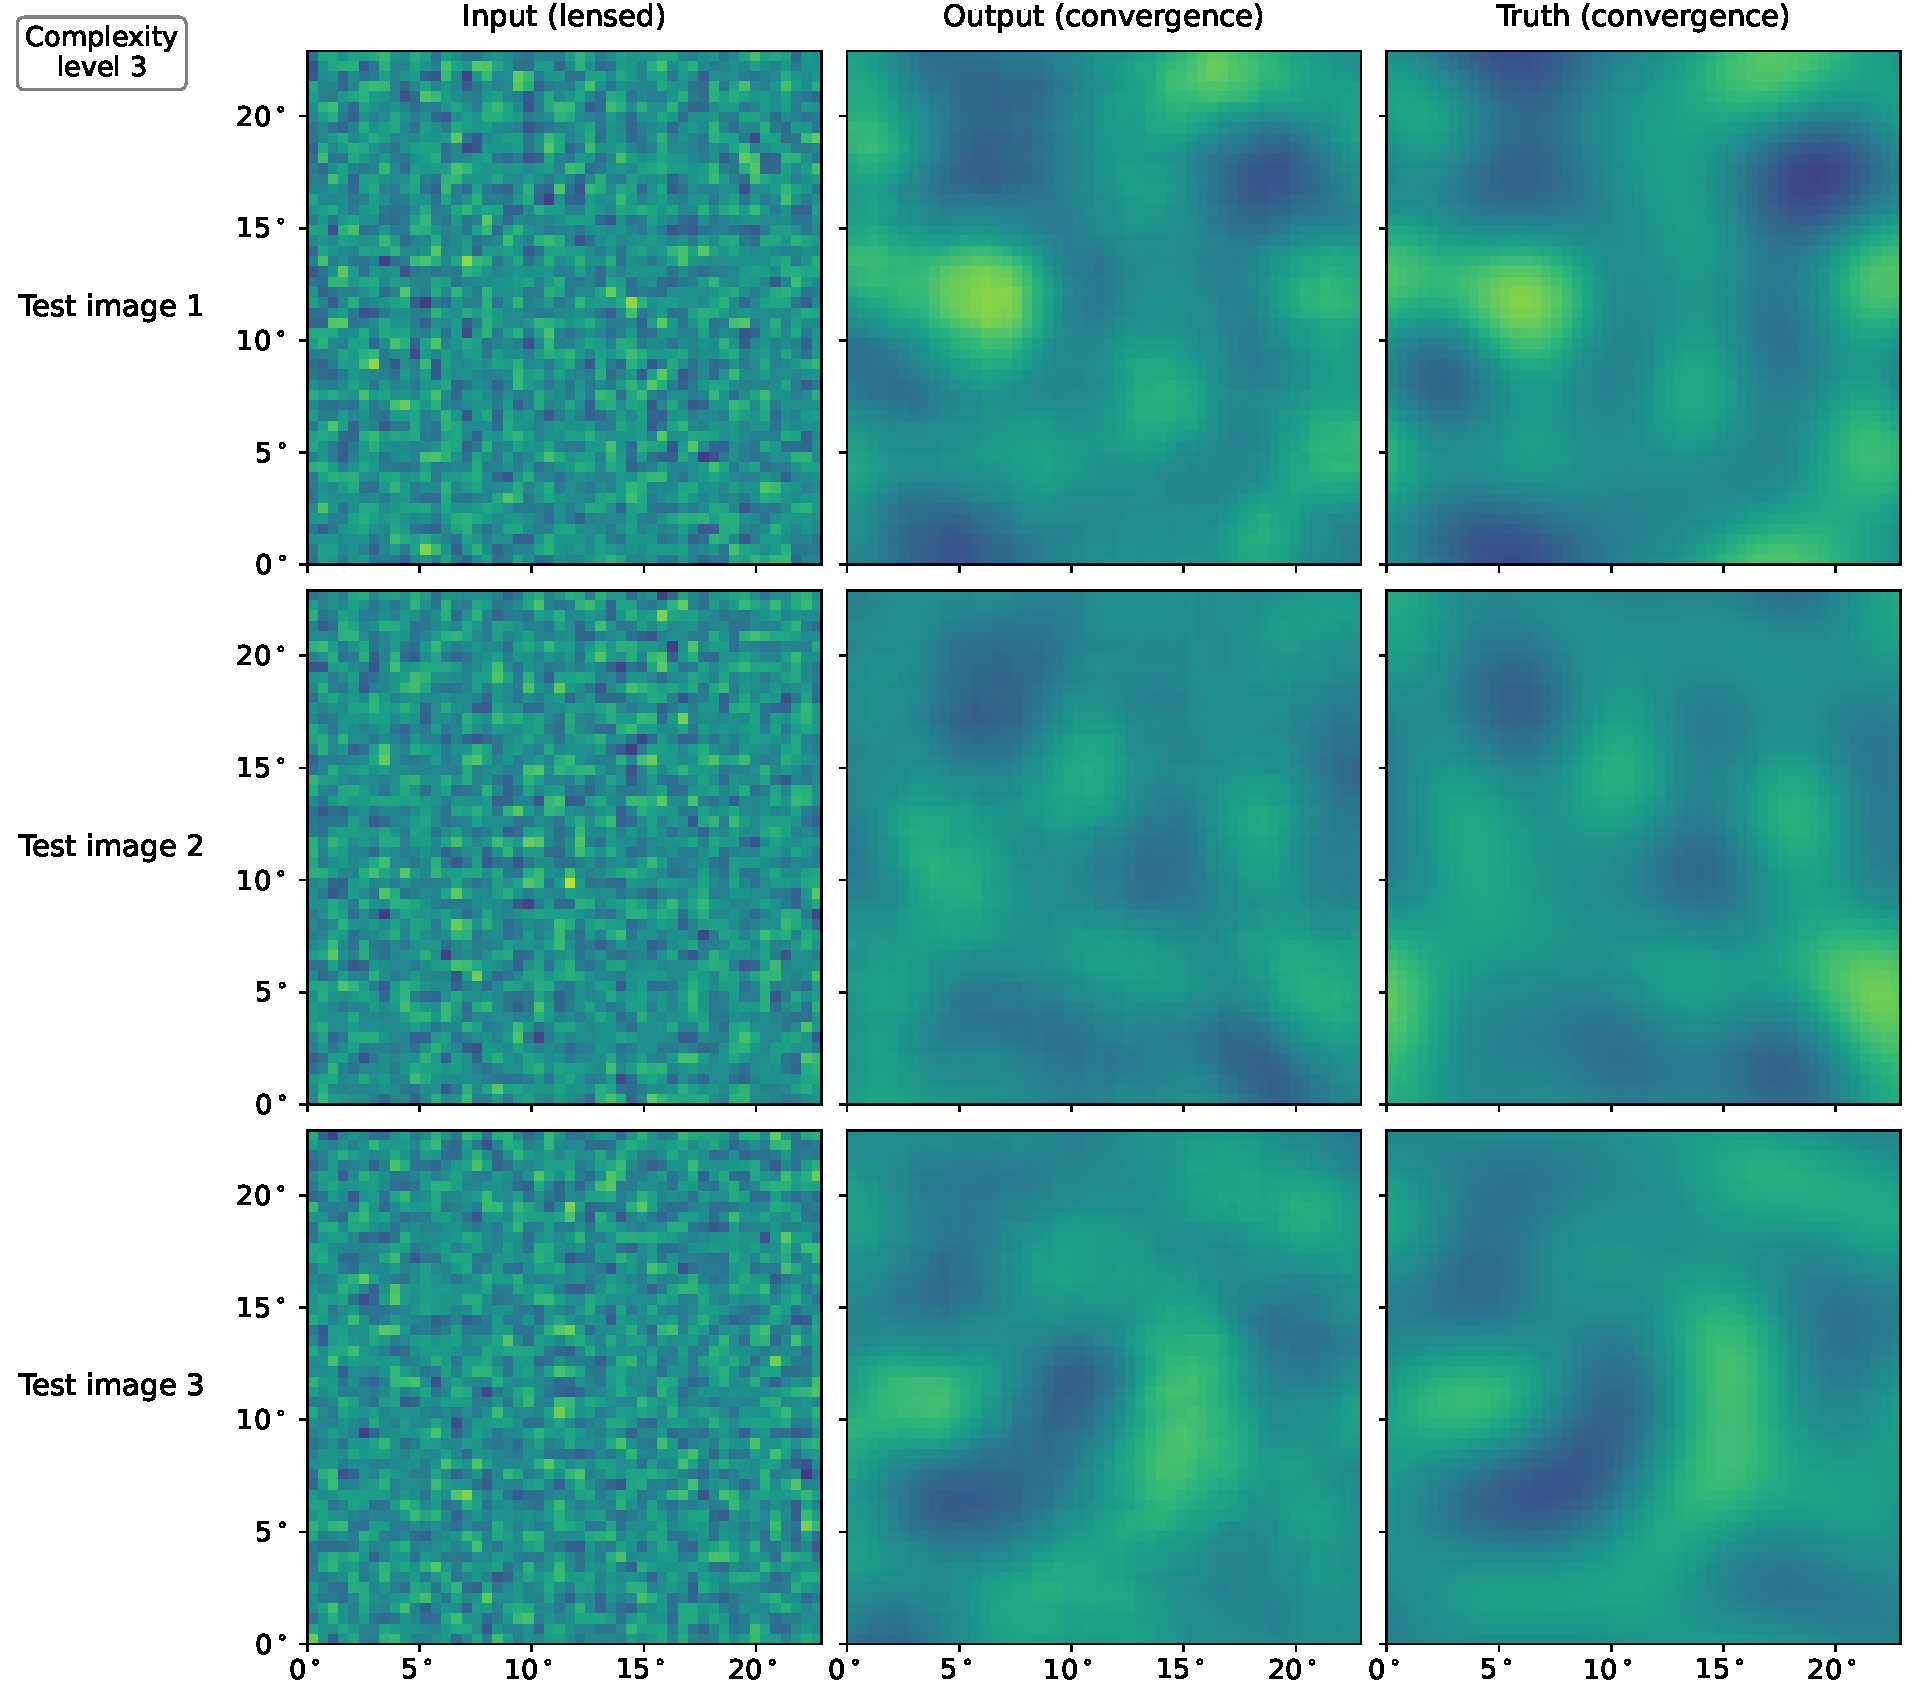
\includegraphics[width=\textwidth]{v3_3x3}
\caption{Performance of the best-performing \texttt{L3\_+32} model for complexity level 3 (described in \autoref{ml_Sec:v3}) on three previously unseen test images. Rows correspond to the different test images, while the columns show, from left to right: the lensed CMB map given as input to the model, the predicted convergence map produced by the model, and the true convergence map that was used to generate the test image in the first column. The model was trained for 50 epochs on a training set of 800 samples augmented by a factor 8, with a validation set of 200 samples which was not augmented.}
\label{ml_Fig:v3_3x3}
\end{figure}

As mentioned above, the baseline model for this complexity level was identical to the best-performing \texttt{L2\_+64} model from complexity level 2, including all aspects of the training setup. Several variations on this model were explored. The standout performers in initial 5-epoch tests were selected for longer 10-epoch tests, which are described below. These standout performers, alongside the baseline model, are as follows:
\begin{itemize}
\item \texttt{L3\_baseline}: \\
% \hspace*{1em}--~64 nodes with a 3$\times$3 kernel; \\
% \hspace*{1em}--~64 nodes with a 3$\times$3 kernel; \\
% \hspace*{1em}--~64 nodes with a 3$\times$3 kernel; \\
% \hspace*{1em}--~64 nodes with a 3$\times$3 kernel; \\
% \hspace*{1em}--~1 node with a 9$\times$9 kernel.
\hspace*{1em}Layers 1--4:~64 nodes with a 3$\times$3 kernel; \\
% \hspace*{1em}Layers 1:4~64 nodes with a 3$\times$3 kernel; \\
% \hspace*{1em}Layers 1:4~64 nodes with a 3$\times$3 kernel; \\
% \hspace*{1em}Layers 1:4~64 nodes with a 3$\times$3 kernel; \\
\hspace*{1em}Layer 5:~~~~~~1 node with a 9$\times$9 kernel.
\item \texttt{L3\_-64}: \\
\hspace*{1em}As \texttt{L3\_baseline}, but without one of the 64-node layers. (This is identical to the \texttt{L2\_baseline} model.)
\item \texttt{L3\_7x7}: \\
\hspace*{1em}As \texttt{L3\_baseline}, but with the final lone kernel having size 7$\times$7.
\item \texttt{L3\_+32}: \\
\hspace*{1em}As \texttt{L3\_baseline}, but with an additional layer of 32 nodes with a 3$\times$3 kernel before the final layer.
\item \texttt{L3\_+64}: \\
\hspace*{1em}As \texttt{L3\_baseline}, but with an additional layer of 64 nodes with a 3$\times$3 kernel before the final layer.
\end{itemize}
The other variations that were explored in the 5-epoch tests included adding and removing different layers, changing numbers of nodes, and changing kernel sizes, but other than the models listed above all variations were found to be either inferior to or similar to the baseline model.

% \begin{figure}[t]
% 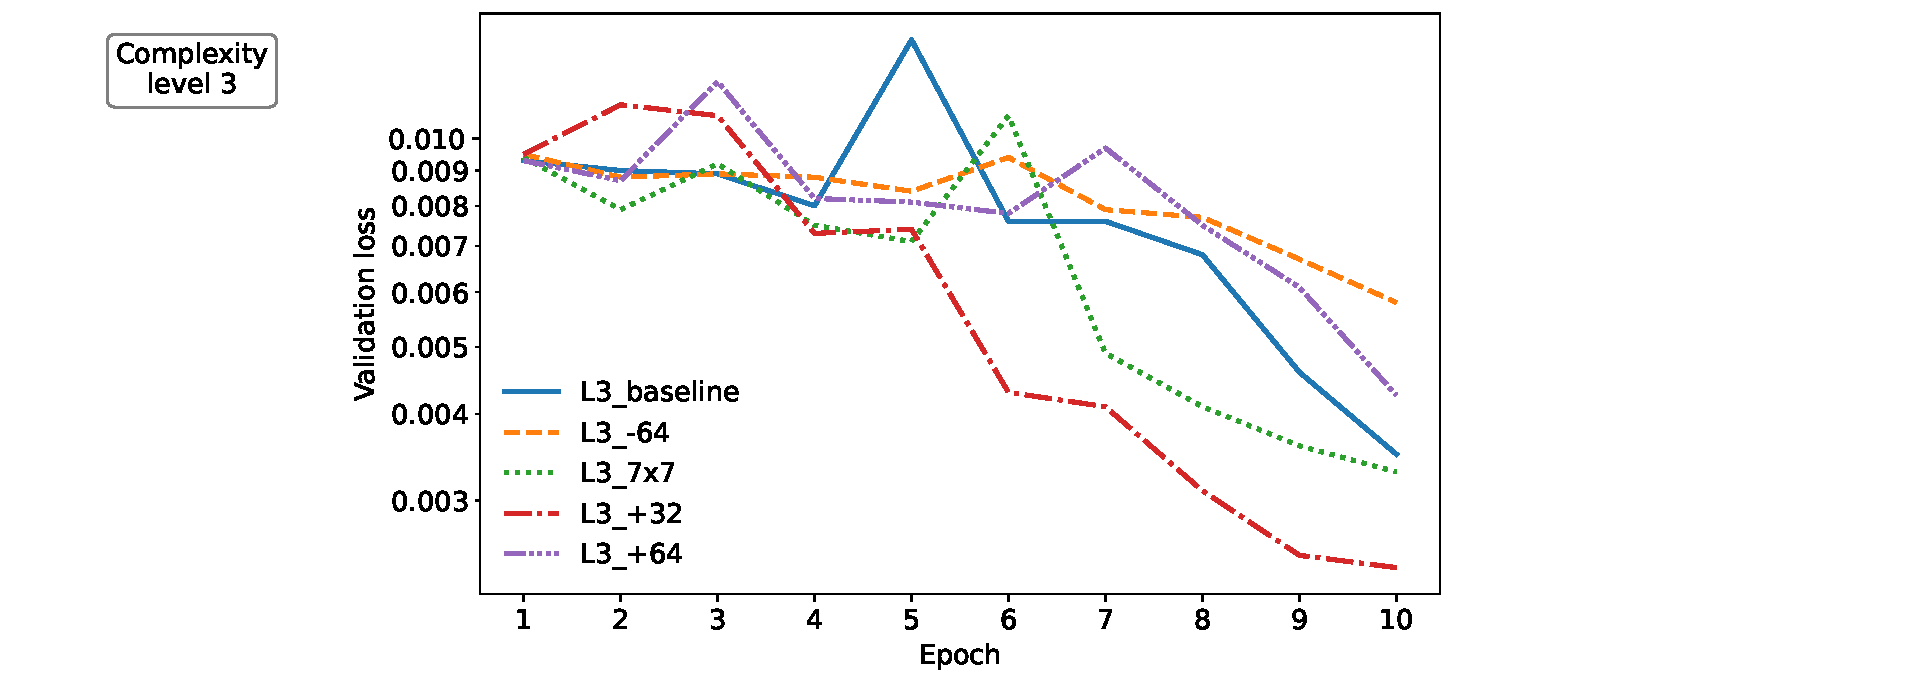
\includegraphics[width=\textwidth]{v3_loss}
% \caption{Validation loss compared between the five best-performing models explored in complexity level 3, which are described in \autoref{ml_Sec:v3}. Each model was trained for 10 epochs on the same training set containing 800 samples prior to augmentation by a factor 8, and validated on 200 different samples which were not augmented.}
% \label{ml_Fig:v3_loss}
% \end{figure}

The five models listed above were each trained for 10 epochs using the same training and validation sets as described above (training size: 800$\times$8; validation size: 200). The validation loss of each model for each training epoch is shown in \autoref{ml_Fig:v3_loss}. There is a clear victory for the \texttt{L3\_+32} model, which achieved a best validation loss of $\mathcal{L}_\text{val} = 2.4 \times 10^{-3}$, while the \texttt{L3\_-64} ($\mathcal{L}_\text{val} = 5.8 \times 10^{-3}$) and \texttt{L3\_+64} ($\mathcal{L}_\text{val} = 4.3 \times 10^{-3}$) models performed worse than the baseline ($\mathcal{L}_\text{val} = 3.5 \times 10^{-3}$). The \texttt{L3\_7x7} model achieved a slight improvement on the baseline, of $\mathcal{L}_\text{val} = 3.3 \times 10^{-3}$. These respective performances were also mirrored in visual tests on a previously unseen test set containing 3 new samples.

% \begin{figure}[tp]
% 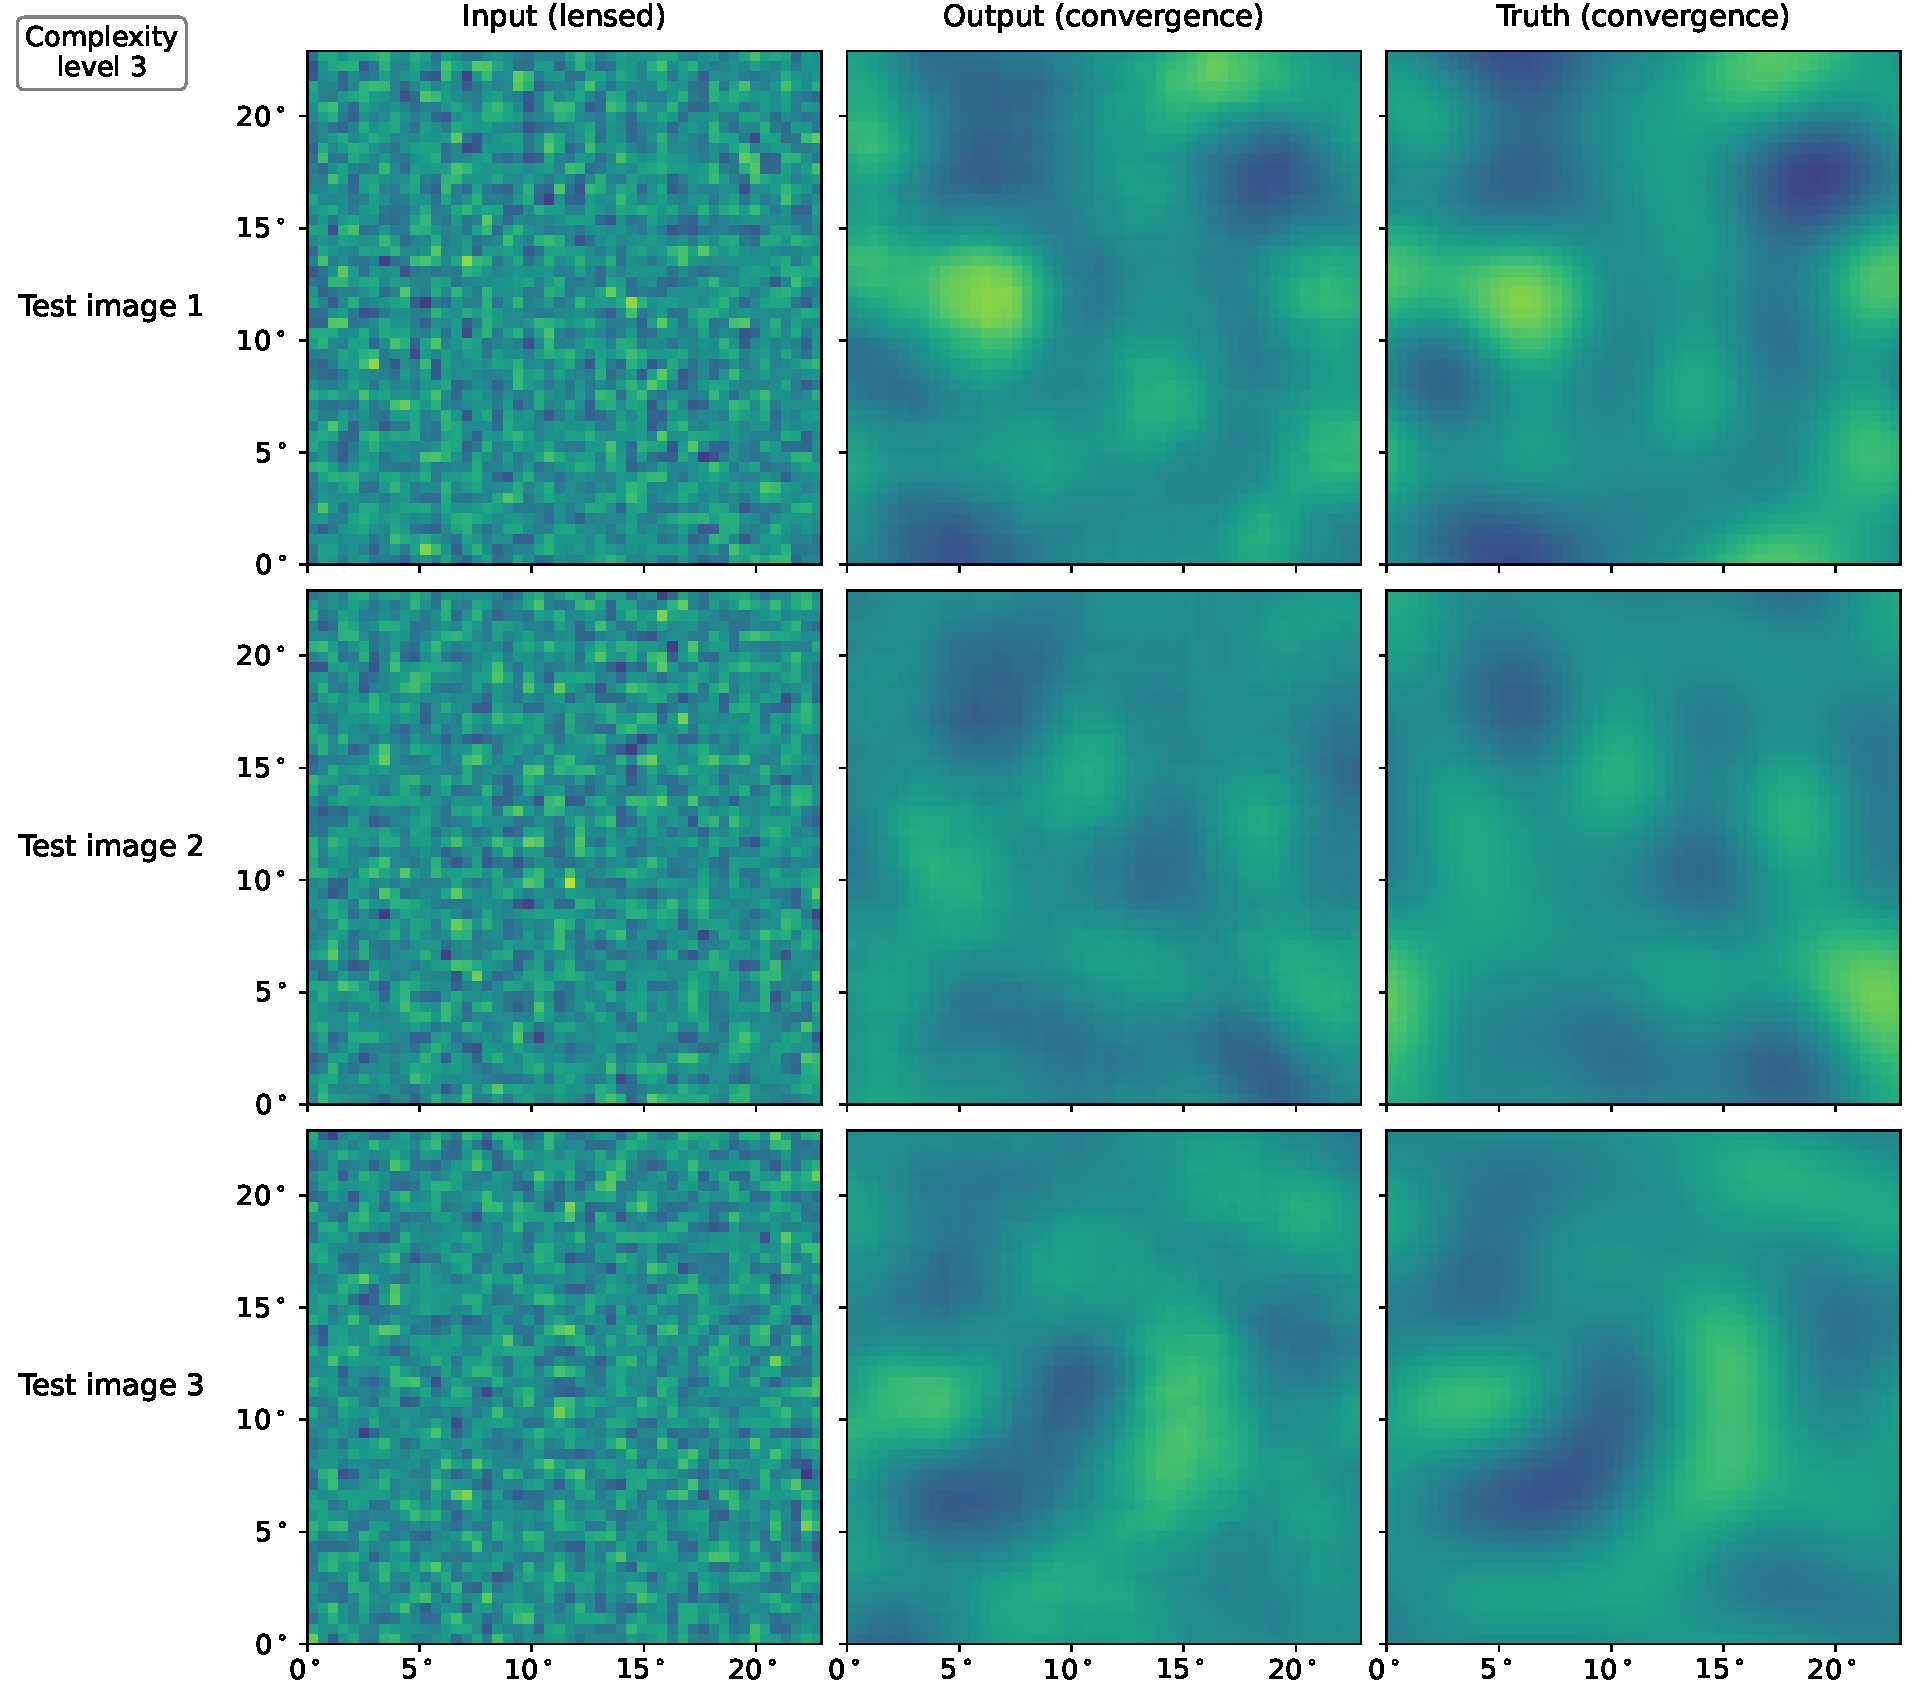
\includegraphics[width=\textwidth]{v3_3x3}
% \caption{Performance of the best-performing \texttt{L3\_+32} model for complexity level 3 (described in \autoref{ml_Sec:v3}) on three previously unseen test images. Rows correspond to the different test images, while the columns show, from left to right: the lensed CMB map given as input to the model, the predicted convergence map produced by the model, and the true convergence map that was used to generate the test image in the first column. The model was trained for 50 epochs on a training set of 800 samples augmented by a factor 8, with a validation set of 200 samples which was not augmented.}
% \label{ml_Fig:v3_3x3}
% \end{figure}

The \texttt{L3\_+32} model was subsequently trained for 50 epochs using the same training and validation set, reaching a best validation loss of $\mathcal{L}_\text{val} = 1.173 \times 10^{-3}$. It was then evaluated on the unseen test set of 3 samples. The resulting predictions for the convergence field are shown alongside the lensed CMB maps and true convergence fields in \autoref{ml_Fig:v3_3x3}. The model achieves a good performance, comparable to complexity level 2 (\autoref{ml_Fig:v2_3x3}), despite the reduction in the lensing exaggeration, which is clearly visible in the left column of \autoref{ml_Fig:v3_3x3} when compared to the visibly exaggerated lensing effect in previous complexity levels (Figures \ref{ml_Fig:v1_3x3} and \ref{ml_Fig:v2_3x3}). This comparable level of performance to complexity level 2 has been achieved without a larger amount of data or more training, and simply required a slightly more complex model architecture.

% \clearpage
\subsection{Complexity level 4: No lensing exaggeration}
\label{ml_Sec:v4}

With a working solution in place for the case of lensing exaggerated by a factor 5, the fourth level of complexity was to now remove the exaggeration entirely. All other aspects of the setup were identical to complexity levels 2--4, which were described in \autoref{ml_Sec:v2}.

The best-performing \texttt{L3\_+32} model from complexity level 3 (\autoref{ml_Sec:v3}) was adopted as the baseline model for level 4, here renamed \texttt{L4\_baseline}. Early testing over 10 epochs with a training set of 800 samples, augmented by a factor 8 following the methods described in \autoref{ml_Sec:data_generation}, failed to recover any features in the true convergence maps. This training set was subsequently enlarged to 1600 samples, but no improvement was detected. As a result, the decision was made to train three models with different depths over a large number of epochs with a large training set. The aim of this approach was twofold: if a large amount of training did not help, it would imply that the lack of data was not the problem and therefore that the models were in some way inappropriate, while if there was a discernible difference between the performance of the three models, this could point to a natural direction in which to seek further improvement.

The three chosen models are as follows:
\begin{itemize}
\item \texttt{L4\_baseline}: \\
% \hspace*{1em}--~64 nodes with a 3$\times$3 kernel; \\
% \hspace*{1em}--~64 nodes with a 3$\times$3 kernel; \\
% \hspace*{1em}--~64 nodes with a 3$\times$3 kernel; \\
% \hspace*{1em}--~64 nodes with a 3$\times$3 kernel; \\
% \hspace*{1em}--~32 nodes with a 3$\times$3 kernel; \\
% \hspace*{1em}--~1 node with a 9$\times$9 kernel.
\hspace*{1em}Layers 1--4:~64 nodes with a 3$\times$3 kernel; \\
% \hspace*{1em}--~64 nodes with a 3$\times$3 kernel; \\
% \hspace*{1em}--~64 nodes with a 3$\times$3 kernel; \\
% \hspace*{1em}--~64 nodes with a 3$\times$3 kernel; \\
\hspace*{1em}Layer 5:~~~~~~32 nodes with a 3$\times$3 kernel; \\
\hspace*{1em}Layer 6:~~~~~~1 node with a 9$\times$9 kernel.
\item \texttt{L4\_-64}: \\
\hspace*{1em}As \texttt{L4\_baseline}, but without one of the 64-node layers.
\item \texttt{L4\_+64}: \\
\hspace*{1em}As \texttt{L4\_baseline}, but with an additional 64-node layer with a 3$\times$3 kernel before the final layer.
\end{itemize}

\begin{figure}[tp]
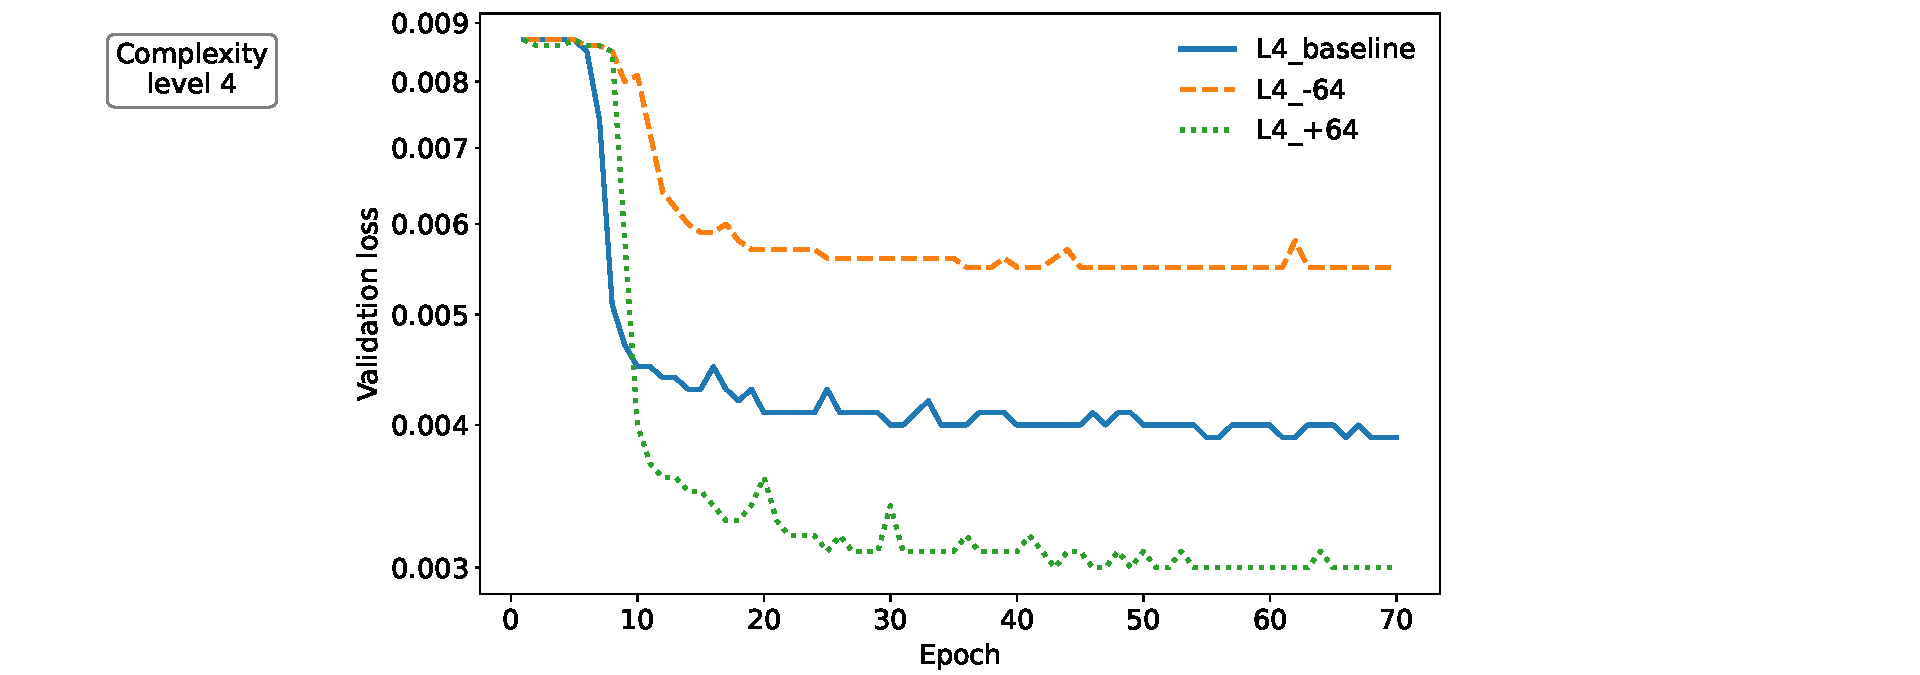
\includegraphics[width=\textwidth]{v4_loss}
\caption{Validation loss compared between the three models explored in complexity level 4, which are described in \autoref{ml_Sec:v4}. Each model was trained for 70 epochs on the same training set containing 9800 samples prior to augmentation by a factor 8, and validated on 200 different samples which were not augmented.}
\label{ml_Fig:v4_loss}
\end{figure}

Each model was trained for 70 epochs on a training set containing 9800 unique samples, augmented by a factor 8 to a final size of 78\,400. A separate validation set of 200 samples was used, which was not augmented. The validation loss during training for each model is shown in \autoref{ml_Fig:v4_loss}, which clearly indicates that more model complexity is beneficial: the more complex \texttt{L4\_+64} model achieved a validation loss of $\mathcal{L}_\text{val} = 2.98 \times 10^{-3}$, while the \texttt{L4\_baseline} model reached $\mathcal{L}_\text{val} = 3.91 \times 10^{-3}$ and the simpler \texttt{L4\_-64} only reached $\mathcal{L}_\text{val} = 5.45 \times 10^{-3}$. All three models converged to a stable validation loss after around 15--30 epochs of training, indicating that they had exhausted the information available in the finite training set.

\begin{figure}[tp]
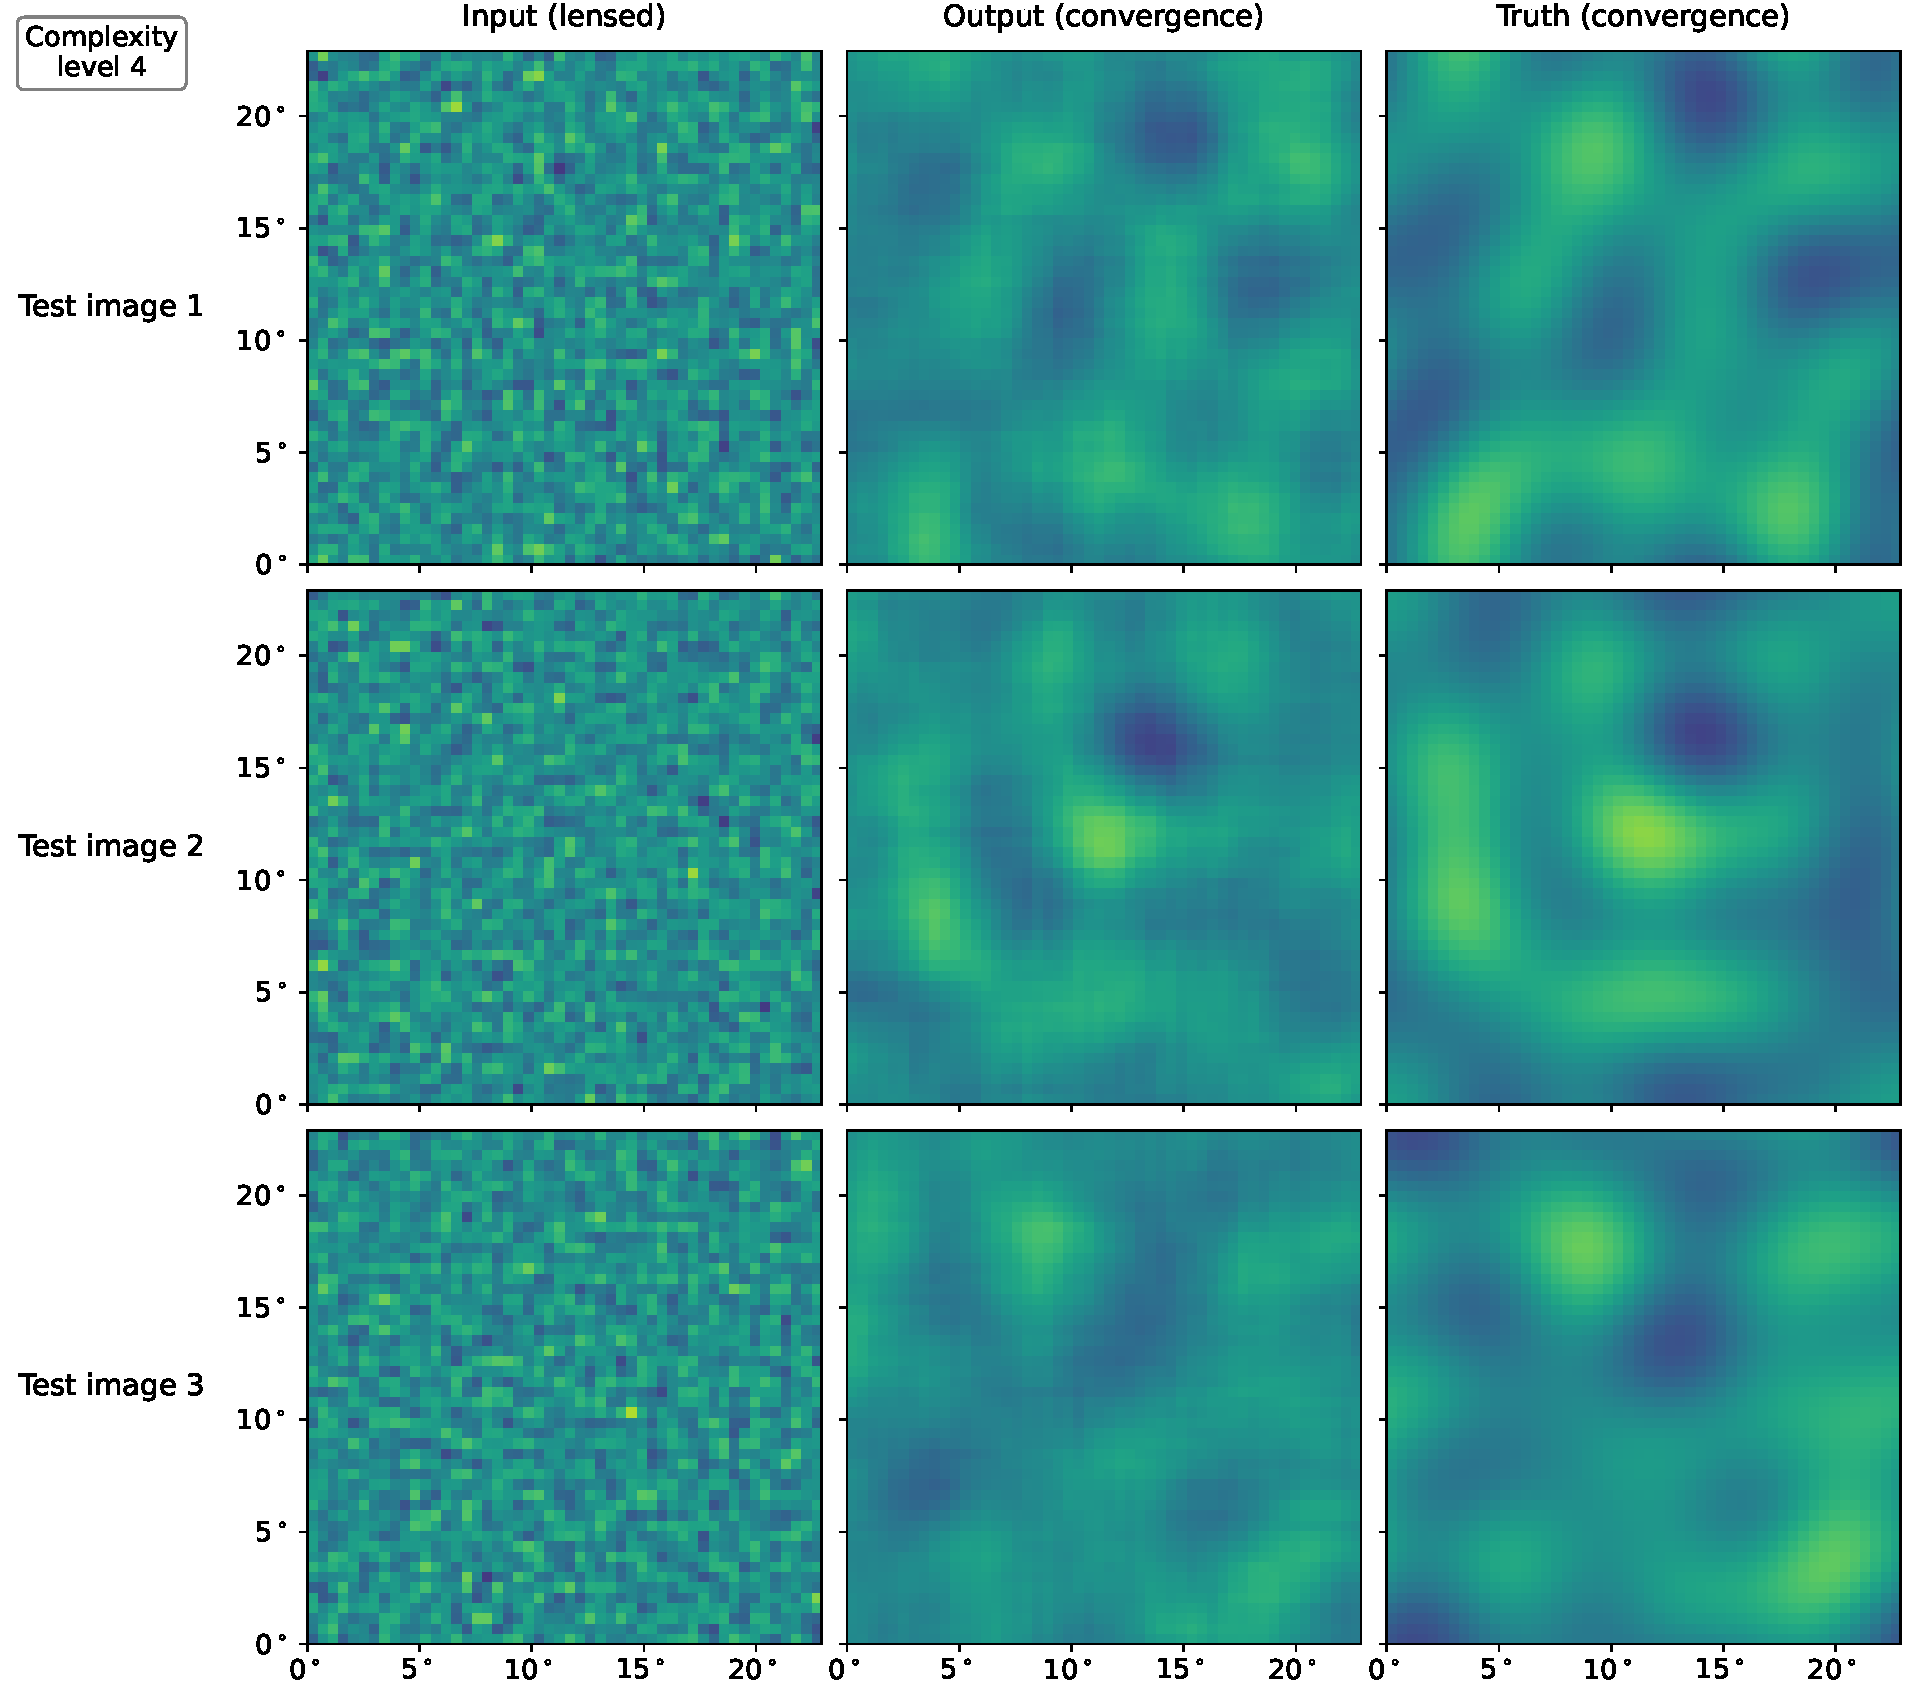
\includegraphics[width=\textwidth]{v4_3x3}
\caption{Performance of the best-performing \texttt{L4\_+64} model for complexity level 4 (described in \autoref{ml_Sec:v4}) on three previously unseen test images. Rows correspond to the different test images, while the columns show, from left to right: the lensed CMB map given as input to the model, the predicted convergence map produced by the model, and the true convergence map that was used to generate the test image in the first column. The model was trained for 70 epochs on a training set of 9800 samples augmented by a factor 8, with a validation set of 200 samples which was not augmented.}
\label{ml_Fig:v4_3x3}
\end{figure}

After training, the three models were each evaluated on a previously unseen test set containing three samples. The results were consistent with the respective validation loss values for each model (\autoref{ml_Fig:v4_loss}), and the \texttt{L4\_+64} was clearly the best performer in terms of the visual correspondence of its predictions to the true convergence field. This is shown in \autoref{ml_Fig:v4_3x3}. The performance is reasonable, although clearly worse than previous complexity levels despite the extra volume of training---both in the size of the training set and the number of training epochs. There are some signs of potential artefacts in the predicted convergence maps. Similar features were observed previously in early tests for the previous complexity levels, but in those cases such features always disappeared with additional training epochs. In this case, the convergence of the validation loss to a steady model for all three models (seen in \autoref{ml_Fig:v4_loss}) indicates that these features should not be expected to disappear with still more training epochs. However, there are clear indications of possible ways in which the performance seen in \autoref{ml_Fig:v4_3x3} might be improved. First, a significant improvement was observed when enlarging the training set from 800 or 1800 samples---which failed to recover any features in the true convergence maps---to 9800 samples, which delivered a much better performance, as seen in \autoref{ml_Fig:v4_3x3}, so it is reasonable to expect that still more data may be able to improve the performance of the three models considered here. Additionally, the comparison between the three models indicates that for this problem a deeper model is more successful, so a natural next step might be to try adding additional layers. However, the level of realism considered at this complexity level is still far below a case that might have practical use, so a progression to the next complexity level takes priority over seeking further improvements to this one.

\subsection{Complexity level 5: Higher resolution, small field of view}
\label{ml_Sec:v5}

The fifth level of complexity was to add resolution, while maintaining the number of pixels at 50$\times$50 in order to retain computational feasibility within reasonable training timescales and memory requirements, both of which rapidly increase with larger images. The field of view was set to a side length of 21.5\,arcmin, which allowed a sub-arcminute pixel size of 0.43\,arcmin, equivalent in pixel area to a HEALPix resolution of $n_\text{side} = 8192$. The low convergence $\ell_\text{max}$ value was raised to a resolution-limited value of $\ell_\text{max} = 24\,575$, while the CMB $\ell_\text{max}$ constraint was removed entirely, being limited by the signal which is negligible above around $\ell \sim 7000$. Such high resolution was partially motivated by the ability to estimate power spectra, for comparison between power spectra estimated from the true and predicted convergence fields.

The baseline model considered for this complexity level was a small variation on the best-performing \texttt{L4\_+64} model from \autoref{ml_Sec:v4}. The single 32-node layer was replaced with a 64-node layer like the other multi-node layers, and the final kernel size was reduced from 9$\times$9 to 3$\times$3, with an aim of being able to recover smaller-scale features in the convergence field. Four variants on this baseline model were considered, which are summarised along with the baseline model as follows:
\begin{itemize}
\item \texttt{L5\_baseline}: \\
% \hspace*{1em}--~64 nodes with a 3$\times$3 kernel; \\
% \hspace*{1em}--~64 nodes with a 3$\times$3 kernel; \\
% \hspace*{1em}--~64 nodes with a 3$\times$3 kernel; \\
% \hspace*{1em}--~64 nodes with a 3$\times$3 kernel; \\
% \hspace*{1em}--~64 nodes with a 3$\times$3 kernel; \\
% \hspace*{1em}--~64 nodes with a 3$\times$3 kernel; \\
% \hspace*{1em}--~1 node with a 3$\times$3 kernel.
\hspace*{1em}Layers 1--6:~64 nodes with a 3$\times$3 kernel; \\
% \hspace*{1em}--~64 nodes with a 3$\times$3 kernel; \\
% \hspace*{1em}--~64 nodes with a 3$\times$3 kernel; \\
% \hspace*{1em}--~64 nodes with a 3$\times$3 kernel; \\
% \hspace*{1em}--~64 nodes with a 3$\times$3 kernel; \\
% \hspace*{1em}--~64 nodes with a 3$\times$3 kernel; \\
\hspace*{1em}Layer 7:~~~~~~1 node with a 3$\times$3 kernel.
\item \texttt{L5\_+64}: \\
\hspace*{1em}As \texttt{L5\_baseline}, but with an additional 64-node layer with a 3$\times$3 kernel before the final layer.
\item \texttt{L5\_7x7}: \\
\hspace*{1em}As \texttt{L5\_baseline}, but with the 3$\times$3 kernel in the final single-node layer replaced with a 7$\times$7 kernel.
\item \texttt{L5\_deep}: \\
% \hspace*{1em}--~32 nodes with a 3$\times$3 kernel; \\
% % \hspace*{1em}--~(Repeated an additional 9 times); \\
% \hspace*{1em}--~32 nodes with a 3$\times$3 kernel; \\
% \hspace*{1em}--~32 nodes with a 3$\times$3 kernel; \\
% \hspace*{1em}--~32 nodes with a 3$\times$3 kernel; \\
% \hspace*{1em}--~32 nodes with a 3$\times$3 kernel; \\
% \hspace*{1em}--~32 nodes with a 3$\times$3 kernel; \\
% \hspace*{1em}--~32 nodes with a 3$\times$3 kernel; \\
% \hspace*{1em}--~32 nodes with a 3$\times$3 kernel; \\
% \hspace*{1em}--~32 nodes with a 3$\times$3 kernel; \\
% \hspace*{1em}--~32 nodes with a 3$\times$3 kernel; \\
% \hspace*{1em}--~1 node with a 3$\times$3 kernel.
%
% \hspace*{1em}~\,1.~32 nodes with a 3$\times$3 kernel; \\
% % \hspace*{1em}--~(Repeated an additional 9 times); \\
% \hspace*{1em}~\,2.~32 nodes with a 3$\times$3 kernel; \\
% \hspace*{1em}~\,3.~32 nodes with a 3$\times$3 kernel; \\
% \hspace*{1em}~\,4.~32 nodes with a 3$\times$3 kernel; \\
% \hspace*{1em}~\,5.~32 nodes with a 3$\times$3 kernel; \\
% \hspace*{1em}~\,6.~32 nodes with a 3$\times$3 kernel; \\
% \hspace*{1em}~\,7.~32 nodes with a 3$\times$3 kernel; \\
% \hspace*{1em}~\,8.~32 nodes with a 3$\times$3 kernel; \\
% \hspace*{1em}~\,9.~32 nodes with a 3$\times$3 kernel; \\
% \hspace*{1em}10.~32 nodes with a 3$\times$3 kernel; \\
% \hspace*{1em}11.~1 node with a 3$\times$3 kernel.
%
\hspace*{1em}Layers 1--10:~32 nodes with a 3$\times$3 kernel; \\
% % \hspace*{1em}--~(Repeated an additional 9 times); \\
% \hspace*{1em}~\,2.~32 nodes with a 3$\times$3 kernel; \\
% \hspace*{1em}~\,3.~32 nodes with a 3$\times$3 kernel; \\
% \hspace*{1em}~\,4.~32 nodes with a 3$\times$3 kernel; \\
% \hspace*{1em}~\,5.~32 nodes with a 3$\times$3 kernel; \\
% \hspace*{1em}~\,6.~32 nodes with a 3$\times$3 kernel; \\
% \hspace*{1em}~\,7.~32 nodes with a 3$\times$3 kernel; \\
% \hspace*{1em}~\,8.~32 nodes with a 3$\times$3 kernel; \\
% \hspace*{1em}~\,9.~32 nodes with a 3$\times$3 kernel; \\
% \hspace*{1em}10.~32 nodes with a 3$\times$3 kernel; \\
\hspace*{1em}Layer 11:~~~~~~1 node with a 3$\times$3 kernel.
%
\item \texttt{L5\_upsampled}: \\
\hspace*{1em}As \texttt{L5\_baseline}, but upsampling by a factor 2 before the first layer, before applying a mean pooling to downsample to the original resolution before the final layer.
\end{itemize}

There were various motivations for exploring these four variations on the baseline model. \texttt{L5\_+64} was motivated by the results of complexity level 4 (\autoref{ml_Sec:v4}), which were clearly suggestive of additional layers achieving higher performance. \texttt{L5\_7x7} was something of an insurance policy in case the reduction of the final kernel size turned out to be detrimental to performance. \texttt{L5\_deep} was motivated by the fact that deeper neural networks are, in general, empirically and theoretically superior to wider networks, since they are better able to model non-linearity in the function that maps from the input to the output \citep[e.g.][]{Safran2016, Lee2020}. Finally, \texttt{L5\_upsampled} was inspired by the original image super-resolution model of \citet{Shi2016} used as the starting point for complexity level 1 in \autoref{ml_Sec:v1}, which used sub-pixel convolution. It seemed plausible that this technique may allow the model to extract smaller-scale information from the lensed CMB maps in this problem.

\begin{figure}[tp]
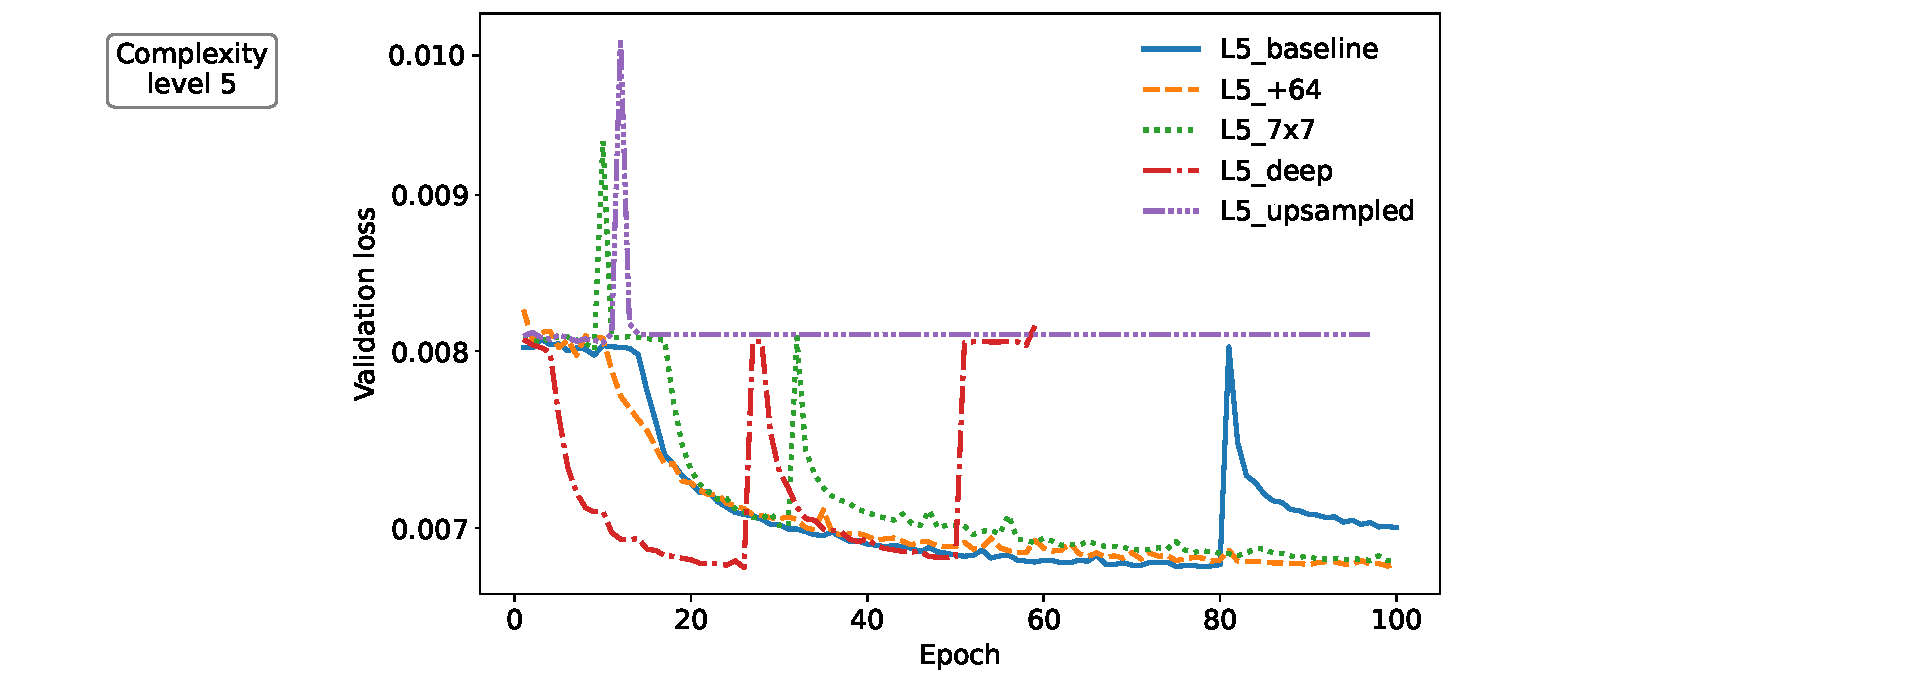
\includegraphics[width=\textwidth]{v5_loss}
\caption{Validation loss compared between the five models explored in complexity level 5, which are described in \autoref{ml_Sec:v5}. Each model was trained for 100 epochs on the same training set containing 9800 samples prior to augmentation by a factor 8, and validated on 200 different samples which were not augmented.}
\label{ml_Fig:v5_loss}
\end{figure}

Each of the five models was trained for 100 epochs, with a training set containing 9800 unique samples, which was augmented by a factor 8, and a validation set containing 200 samples, which was not augmented. The validation loss for each model throughout training is shown in \autoref{ml_Fig:v5_loss}. The best-performing model was \texttt{L5\_+64}, reaching a minimum validation loss of $\mathcal{L}_\text{val} = 6.80 \times 10^{-3}$. Three other models performed similarly well: \texttt{L5\_baseline} and \texttt{L5\_deep} also reached $\mathcal{L}_\text{val} = 6.80 \times 10^{-3}$, while \texttt{L5\_deep} was slightly behind at $\mathcal{L}_\text{val} = 6.83 \times 10^{-3}$. However, all three of these models exhibited a strange behaviour of a sudden divergence in the validation loss followed by a slow convergence back towards the initial minimum. In the case of the {L5\_deep} model, a second divergence was observed, at which point the model weights became infinite and training ceased; this is why the corresponding line in \autoref{ml_Fig:v5_loss} stops suddenly at around 60 epochs. Similar features were found in the training loss. This behaviour is not currently understood, since divergent weights should not be permitted by the update rule for the Adam optimiser (\autoref{ml_Eqn:theta_update_rule}). This issue is discussed further in \autoref{ml_Sec:discussion}. Meanwhile, the performance of the \texttt{L5\_upsampled} model was poor, plateauing at $\mathcal{L}_\text{val} = 8.05 \times 10^{-3}$.

\begin{figure}[tp]
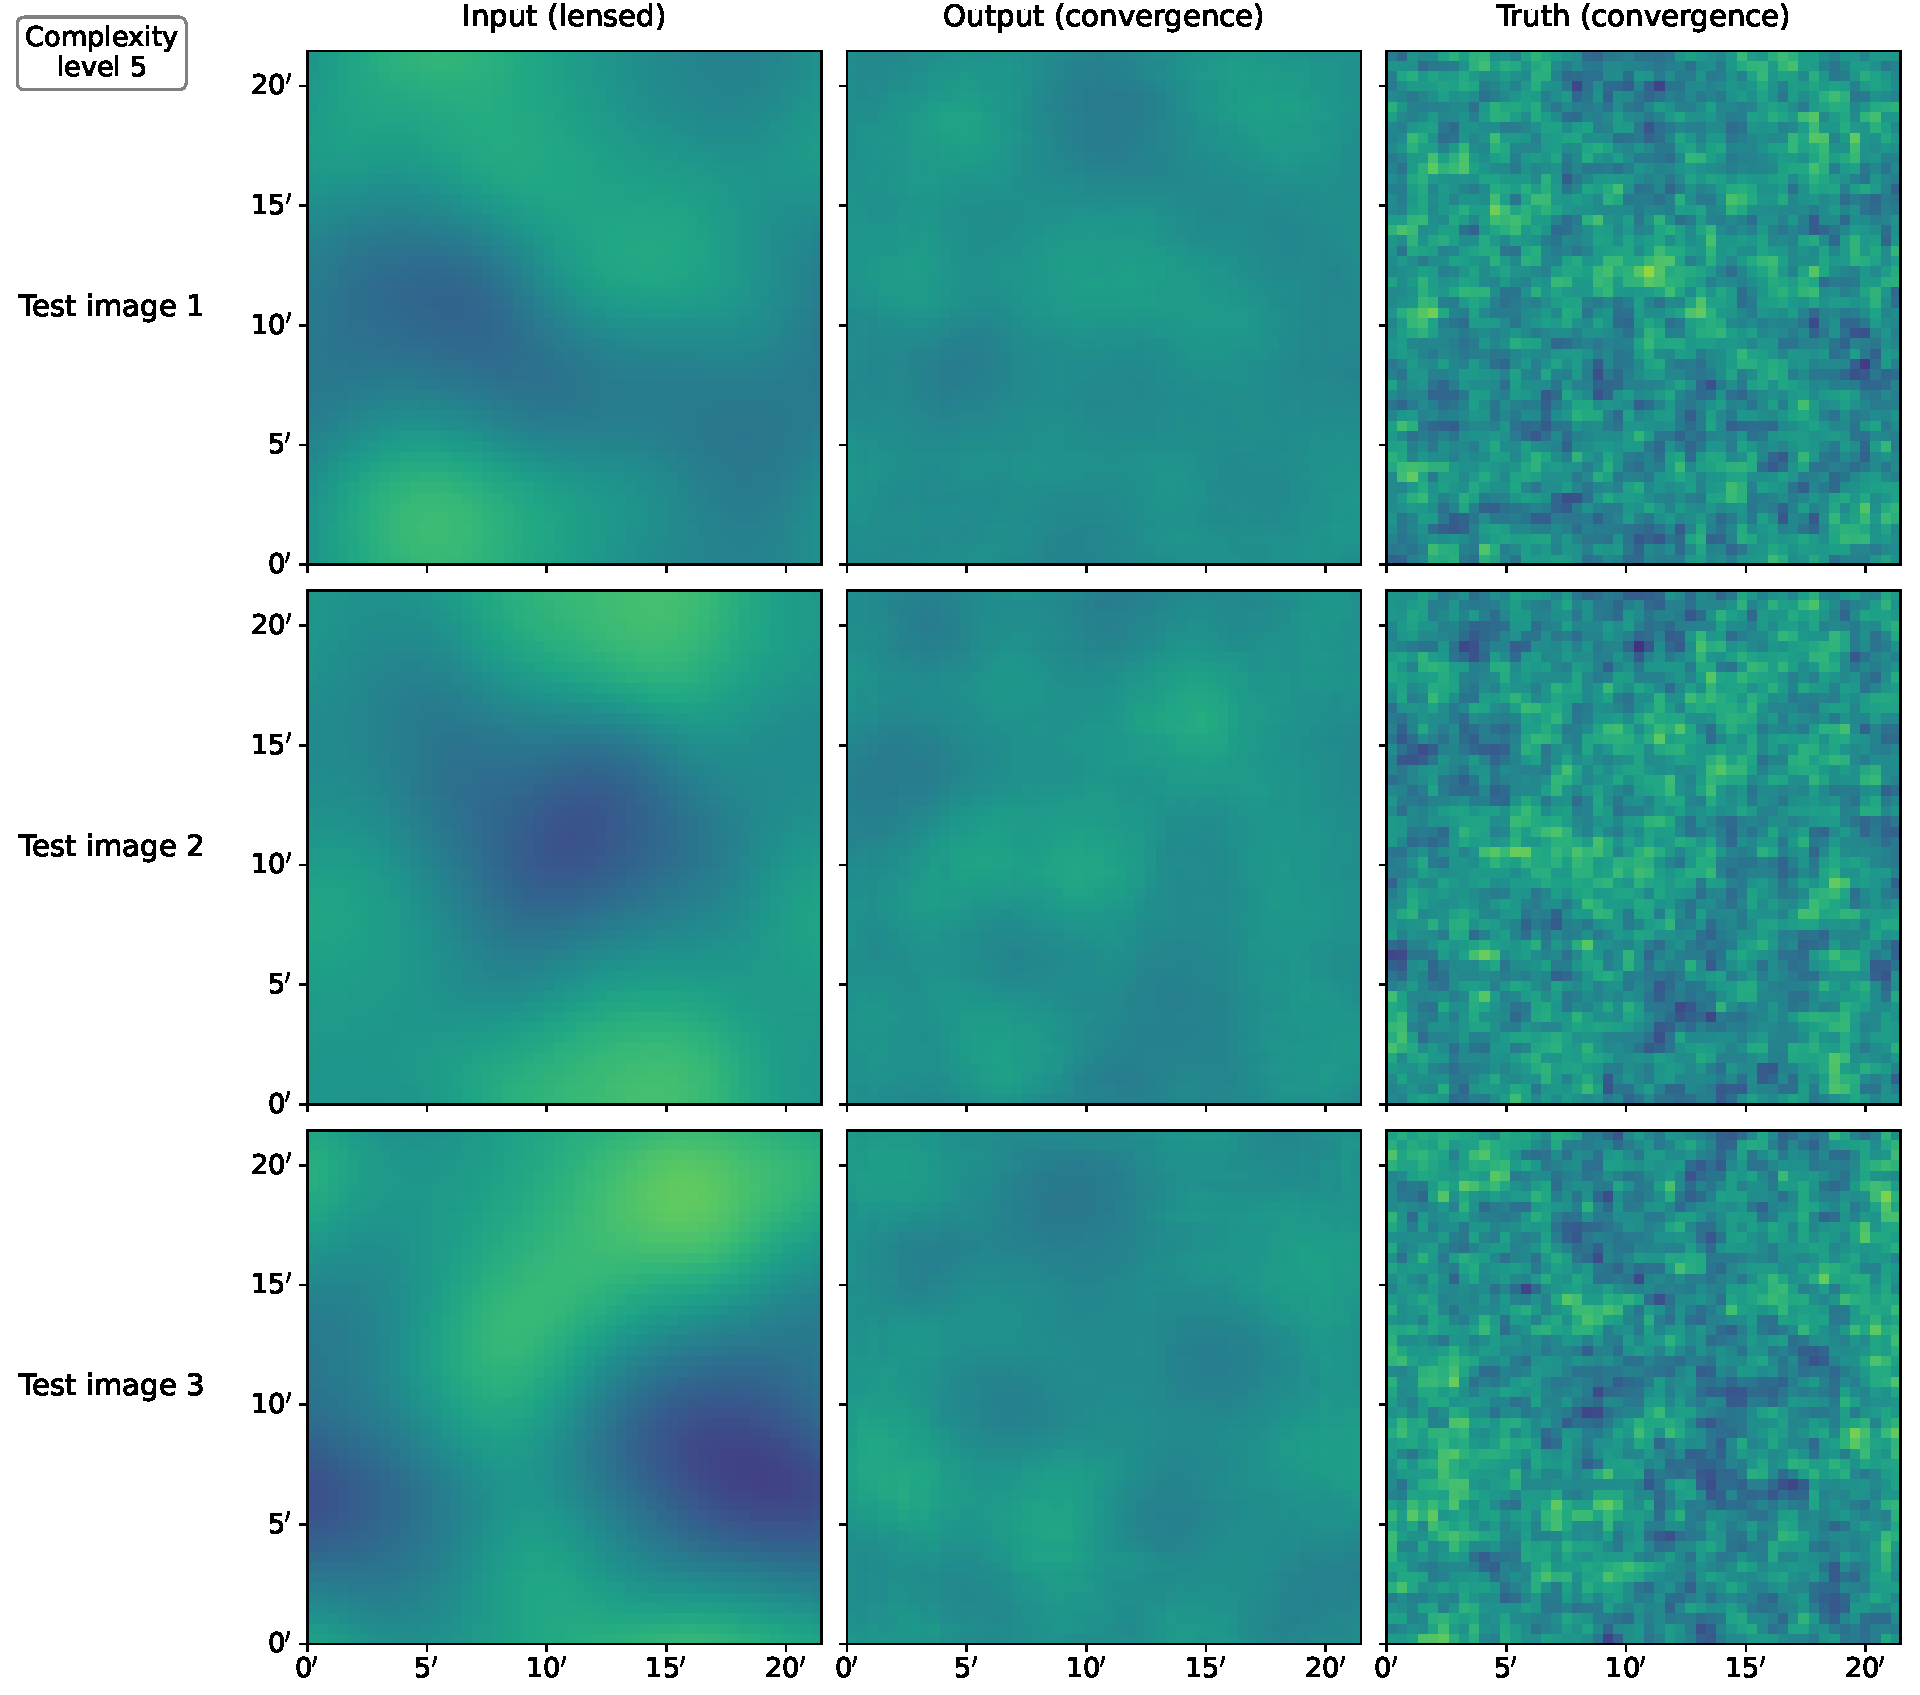
\includegraphics[width=\textwidth]{v5_3x3}
\caption{Performance of the best-performing \texttt{L5\_+64} model for complexity level 5 (described in \autoref{ml_Sec:v5}) on three previously unseen test images. Rows correspond to the different test images, while the columns show, from left to right: the lensed CMB map given as input to the model, the predicted convergence map produced by the model, and the true convergence map that was used to generate the test image in the first column. The model was trained for 100 epochs on a training set of 9800 samples augmented by a factor 8, with a validation set of 200 samples which was not augmented.}
\label{ml_Fig:v5_3x3}
\end{figure}

Each model was evaluated using a test set of three previously unseen images. For each model, the weights corresponding to the minimum validation loss were used---for instance, the \texttt{L5\_baseline} model was evaluated using its weights at around epoch 80, prior to its subsequent divergence (seen in \autoref{ml_Fig:v5_loss}). The results were consistent with the respective validation losses: a similar performance was observed between all models except \texttt{L5\_upsampled}, which did not appear to recover any features in the true convergence maps. The visual test results for the \texttt{L5\_+64} model are shown in \autoref{ml_Fig:v5_3x3}. Small-scale features are absent, but there is an apparent correspondence between the estimated and true convergence fields on larger scales.

\begin{figure}[tp]
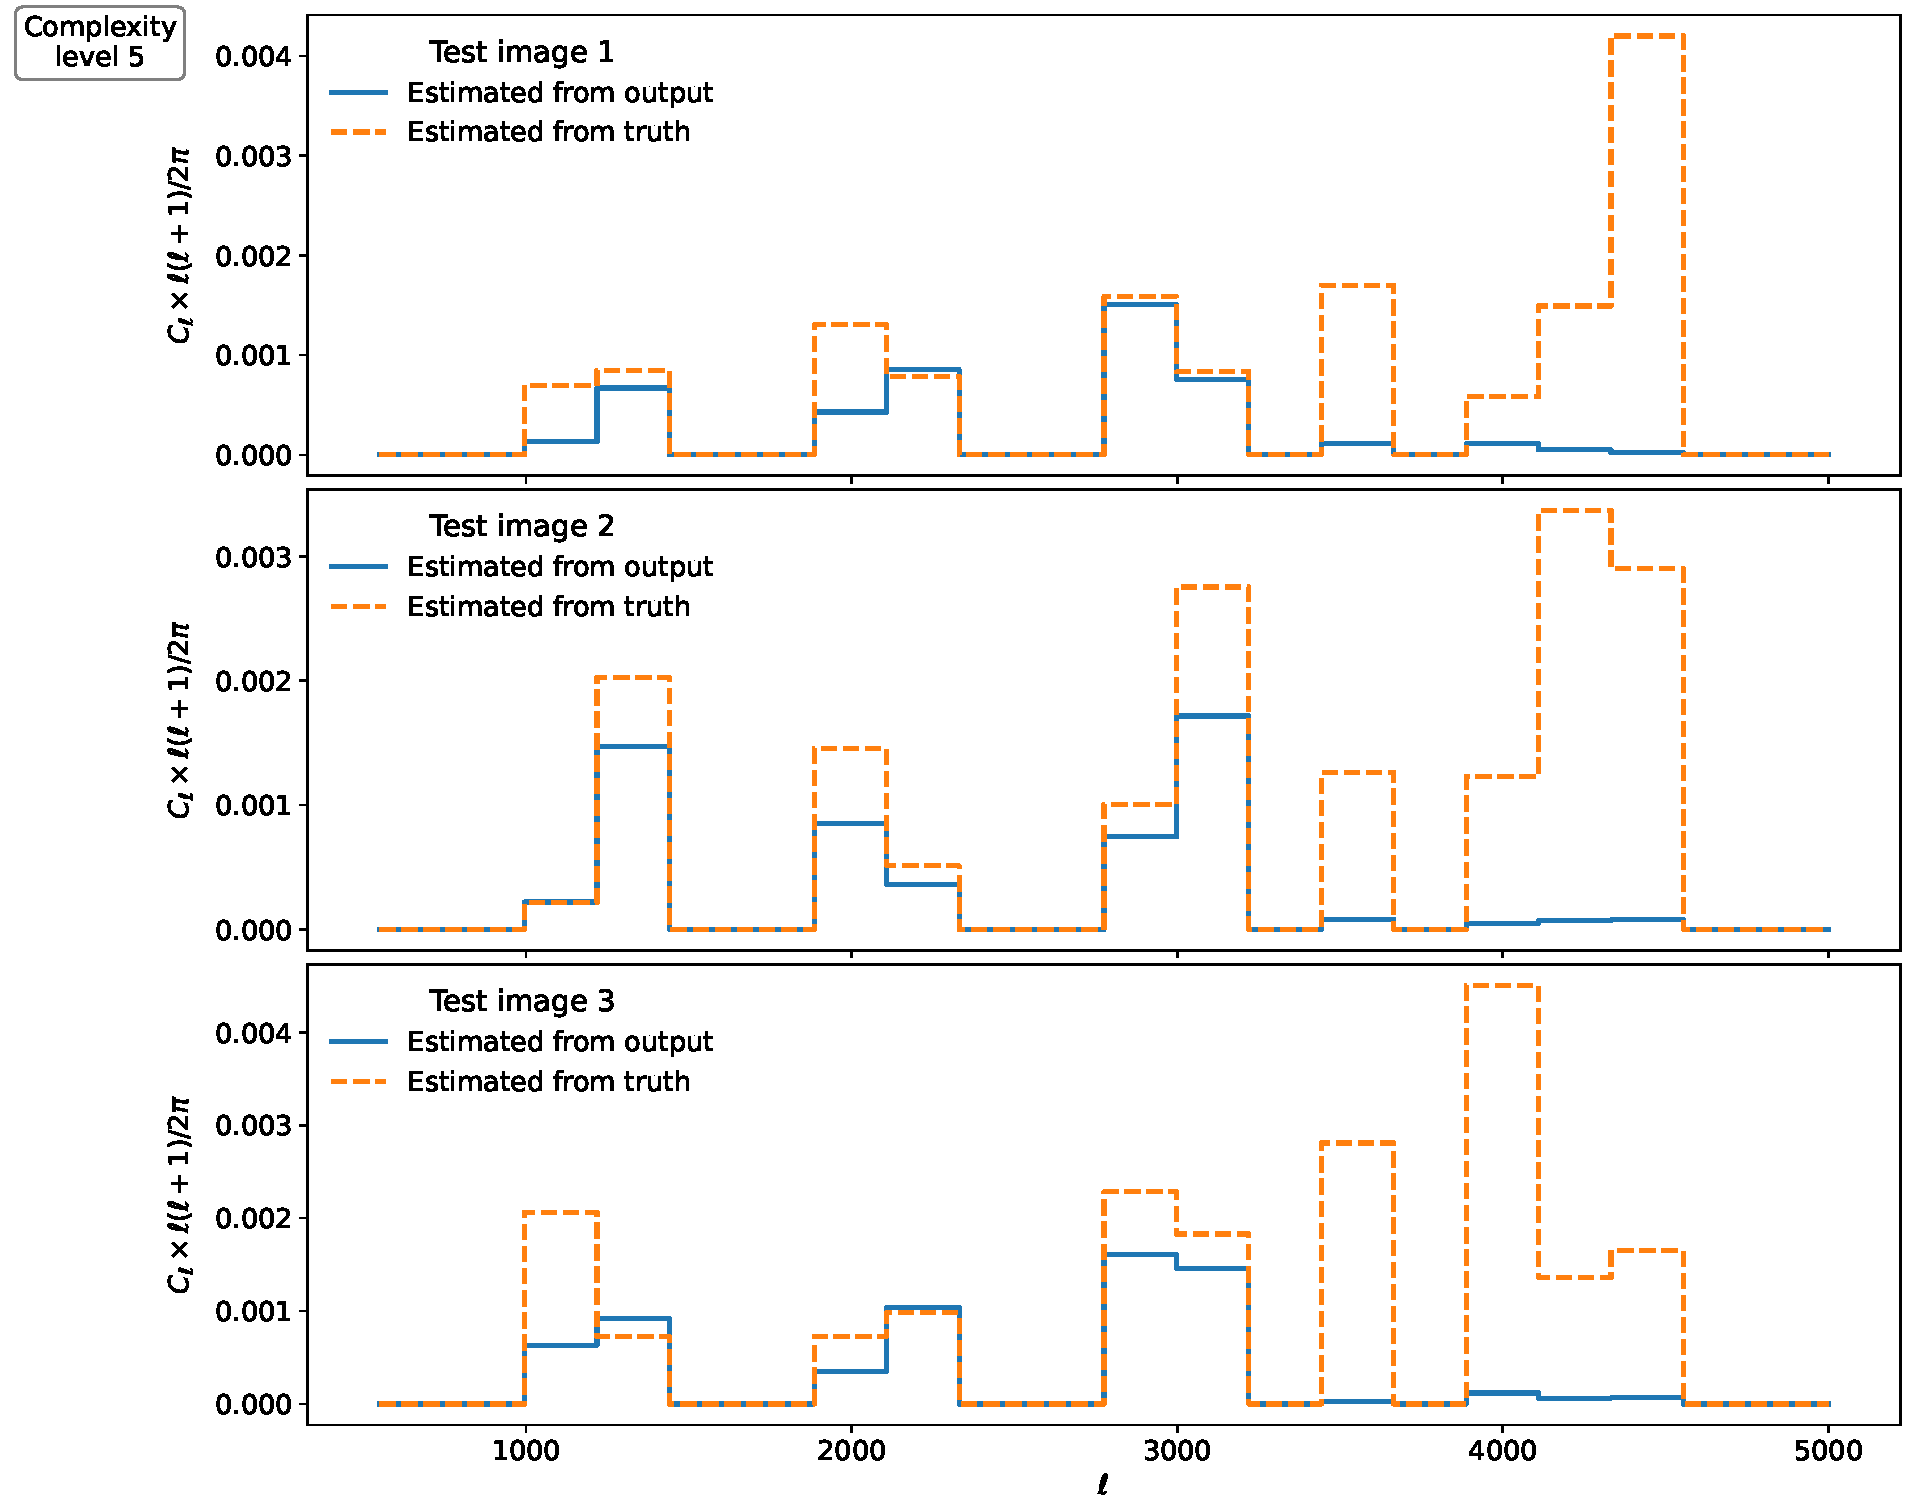
\includegraphics[width=\textwidth]{v5_cls}
\caption{Power spectra estimated from the convergence maps shown in \autoref{ml_Fig:v5_3x3}. Rows correspond to the three different test images. The blue solid line shows the power spectrum estimated from the predicted convergence map output by the convolutional neural network, while the orange dashed line shows the power spectrum estimated from the true convergence map. Results shown are for the \texttt{L5\_+64} model for complexity level 5 (described in \autoref{ml_Sec:v5}). The model was trained for 100 epochs on a training set of 9800 samples augmented by a factor 8, with a validation set of 200 samples which was not augmented.}
\label{ml_Fig:v5_cls}
\end{figure}

For the first time, it was possible with this complexity level to estimate power spectra from the true and predicted convergence fields, using \texttt{NaMaster}. These are shown for the three test images and the \texttt{L5\_+64} model in \autoref{ml_Fig:v5_cls}. It is clear that the model is able to recover large-scale features in the power spectrum quite well, but that small-scale features (above around $\ell \sim 3500$) are missed entirely. This is consistent with the visual observations from the maps in \autoref{ml_Fig:v5_3x3}. Similar performance was found for all other models except \texttt{L5\_upsampled}, which did not recover any power.

It is perhaps unsurprising that smaller-scale features in the convergence maps are not recovered, given the lack of visible features on such scales in the input lensed CMB maps (left column of \autoref{ml_Fig:v5_3x3}). This motivated a return to a larger field of view, in order to regain the degree-scale features in the CMB and convergence fields. This is explored in \autoref{ml_Sec:v6} below.
% Ideally this would be done while retaining sub-arcminute pixel scales, since deflections are on this sort of scale. However, this would require a number of pixels so large as to cause a number of computational problems. As a result, an intermediate setup was explored, which is described in \autoref{ml_Sec:v6} below.

\subsection{Complexity level 6: Higher resolution, wide field of view}
\label{ml_Sec:v6}

As mentioned above, for the next complexity level it was chosen to return to a larger field of view, in order to regain the degree-scale features in the CMB and convergence fields. Ideally this would be done while retaining sub-arcminute pixel size, since typical deflections are around this scale \citep[e.g.][]{Lewis2006}. However, this would require a large number of pixels, of order 1000 along each side. Initial testing revealed that this was not computationally feasible with the available resources, due to memory requirements during training. As a result, an intermediate setup was instead explored, using 100 pixels along each side with a 10 degree field of view, giving a pixel size of 6 arcmin along each side. Unlike previous complexity levels, there is no exact equivalent HEALPix resolution in terms of pixel area, but it is approximately equivalent to $n_\text{side} = 512$. No explicit $\ell_\text{max}$ cut was applied to either the CMB or convergence fields, but both were limited by resolution to an effective $\ell_\text{max} \sim 1535$.

Even this modest increase of total number of pixels by a factor of 4 (2 along each side) required the introduction of \texttt{Keras} \texttt{Sequence} objects to load only a part of the training data into memory at any given point during training, as described in \autoref{ml_Sec:model_building_training}.

Motivated by the ability of the \texttt{L5\_deep} model to quickly reach a low minimum validation loss in \autoref{ml_Sec:v5} (the subsequent unexplained divergence notwithstanding), and by the general preference towards deeper models in the literature described in that section, the baseline model was chosen to contain 12 convolutional layers of 32 nodes each, plus the usual final single-node convolutional layer. The final kernel size of 3$\times$3 used in \autoref{ml_Sec:v5} was retained, since the goal of recovering small-scale features is the same. All other aspects of the model, and the optimiser used for training, were identical to previous complexity levels. Two additional model variations with increasing depth and decreasing width were explored. These, along with the baseline model, are summarised as follows:
\begin{itemize}
\item \texttt{L6\_baseline}: \\
\hspace*{1em}Layers 1--12:~32 nodes with a 3$\times$3 kernel; \\
\hspace*{1em}Layer 13:~~~~~~1 node with a 3$\times$3 kernel.
\item \texttt{L6\_x2depth}: \\
% \hspace*{1em}1--24.~16 nodes with a 3$\times$3 kernel; \\
% \hspace*{1em}~~~\,25.~1 node with a 3$\times$3 kernel.
\hspace*{1em}Layers 1--24:~16 nodes with a 3$\times$3 kernel; \\
\hspace*{1em}Layer 25:~~~~~~1 node with a 3$\times$3 kernel.
\item \texttt{L6\_x4depth}: \\
% \hspace*{1em}1--48.~8 nodes with a 3$\times$3 kernel; \\
% \hspace*{1em}~~~\,49.~1 node with a 3$\times$3 kernel.
\hspace*{1em}Layers 1--48:~8 nodes with a 3$\times$3 kernel; \\
\hspace*{1em}Layer 49:~~~~~~1 node with a 3$\times$3 kernel.
\end{itemize}

\begin{figure}[tp]
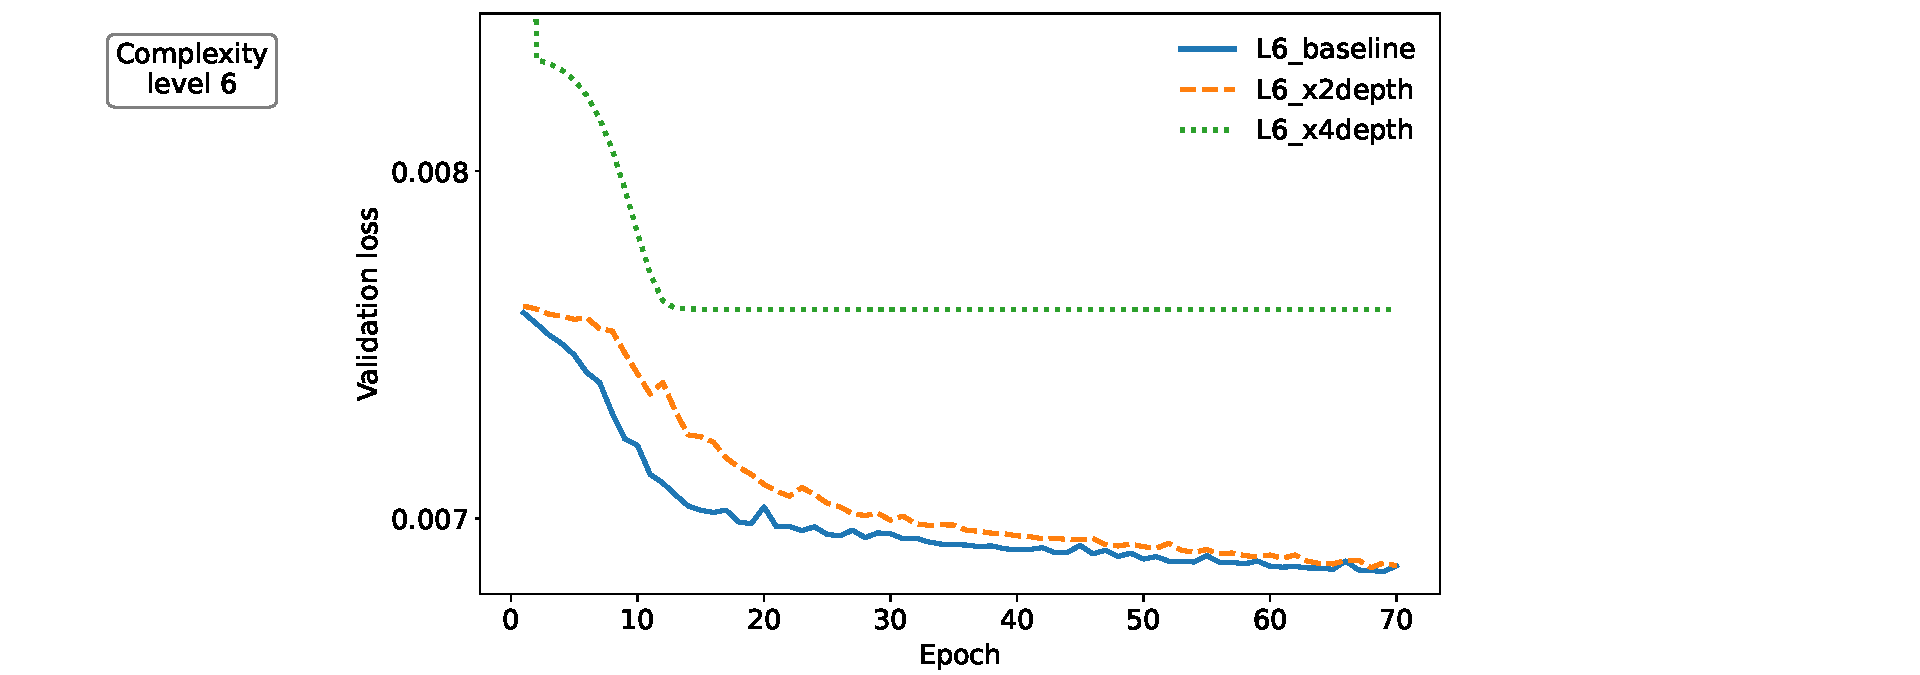
\includegraphics[width=\textwidth]{v6_loss}
\caption{Validation loss compared between the three models explored in complexity level 6, which are described in \autoref{ml_Sec:v6}. Each model was trained for 70 epochs on the same training set containing 9800 samples prior to augmentation by a factor 8, and validated on 200 different samples which were not augmented.}
\label{ml_Fig:v6_loss}
\end{figure}

Each model was trained for 70 epochs on a training set containing 9\,800 samples, which was augmented by a factor 8 using the methods described in \autoref{ml_Sec:data_generation}, and validated using a validation set containing 200 samples, which was not augmented. The validation loss of each model throughout training is shown in \autoref{ml_Fig:v6_loss}. The \texttt{L6\_baseline} in fact performed the best throughout the whole training process, reaching a validation loss of $\mathcal{L}_\text{val} = 6.86 \times 10^{-3}$, although by epoch 70 the performance of the \texttt{L6\_x2depth} model was similar, reaching $\mathcal{L}_\text{val} = 6.87 \times 10^{-3}$. The \texttt{L6\_x4depth} model performed most poorly, with the validation loss plateauing at $\mathcal{L}_\text{val} = 7.59 \times 10^{-3}$.

\begin{figure}[tp]
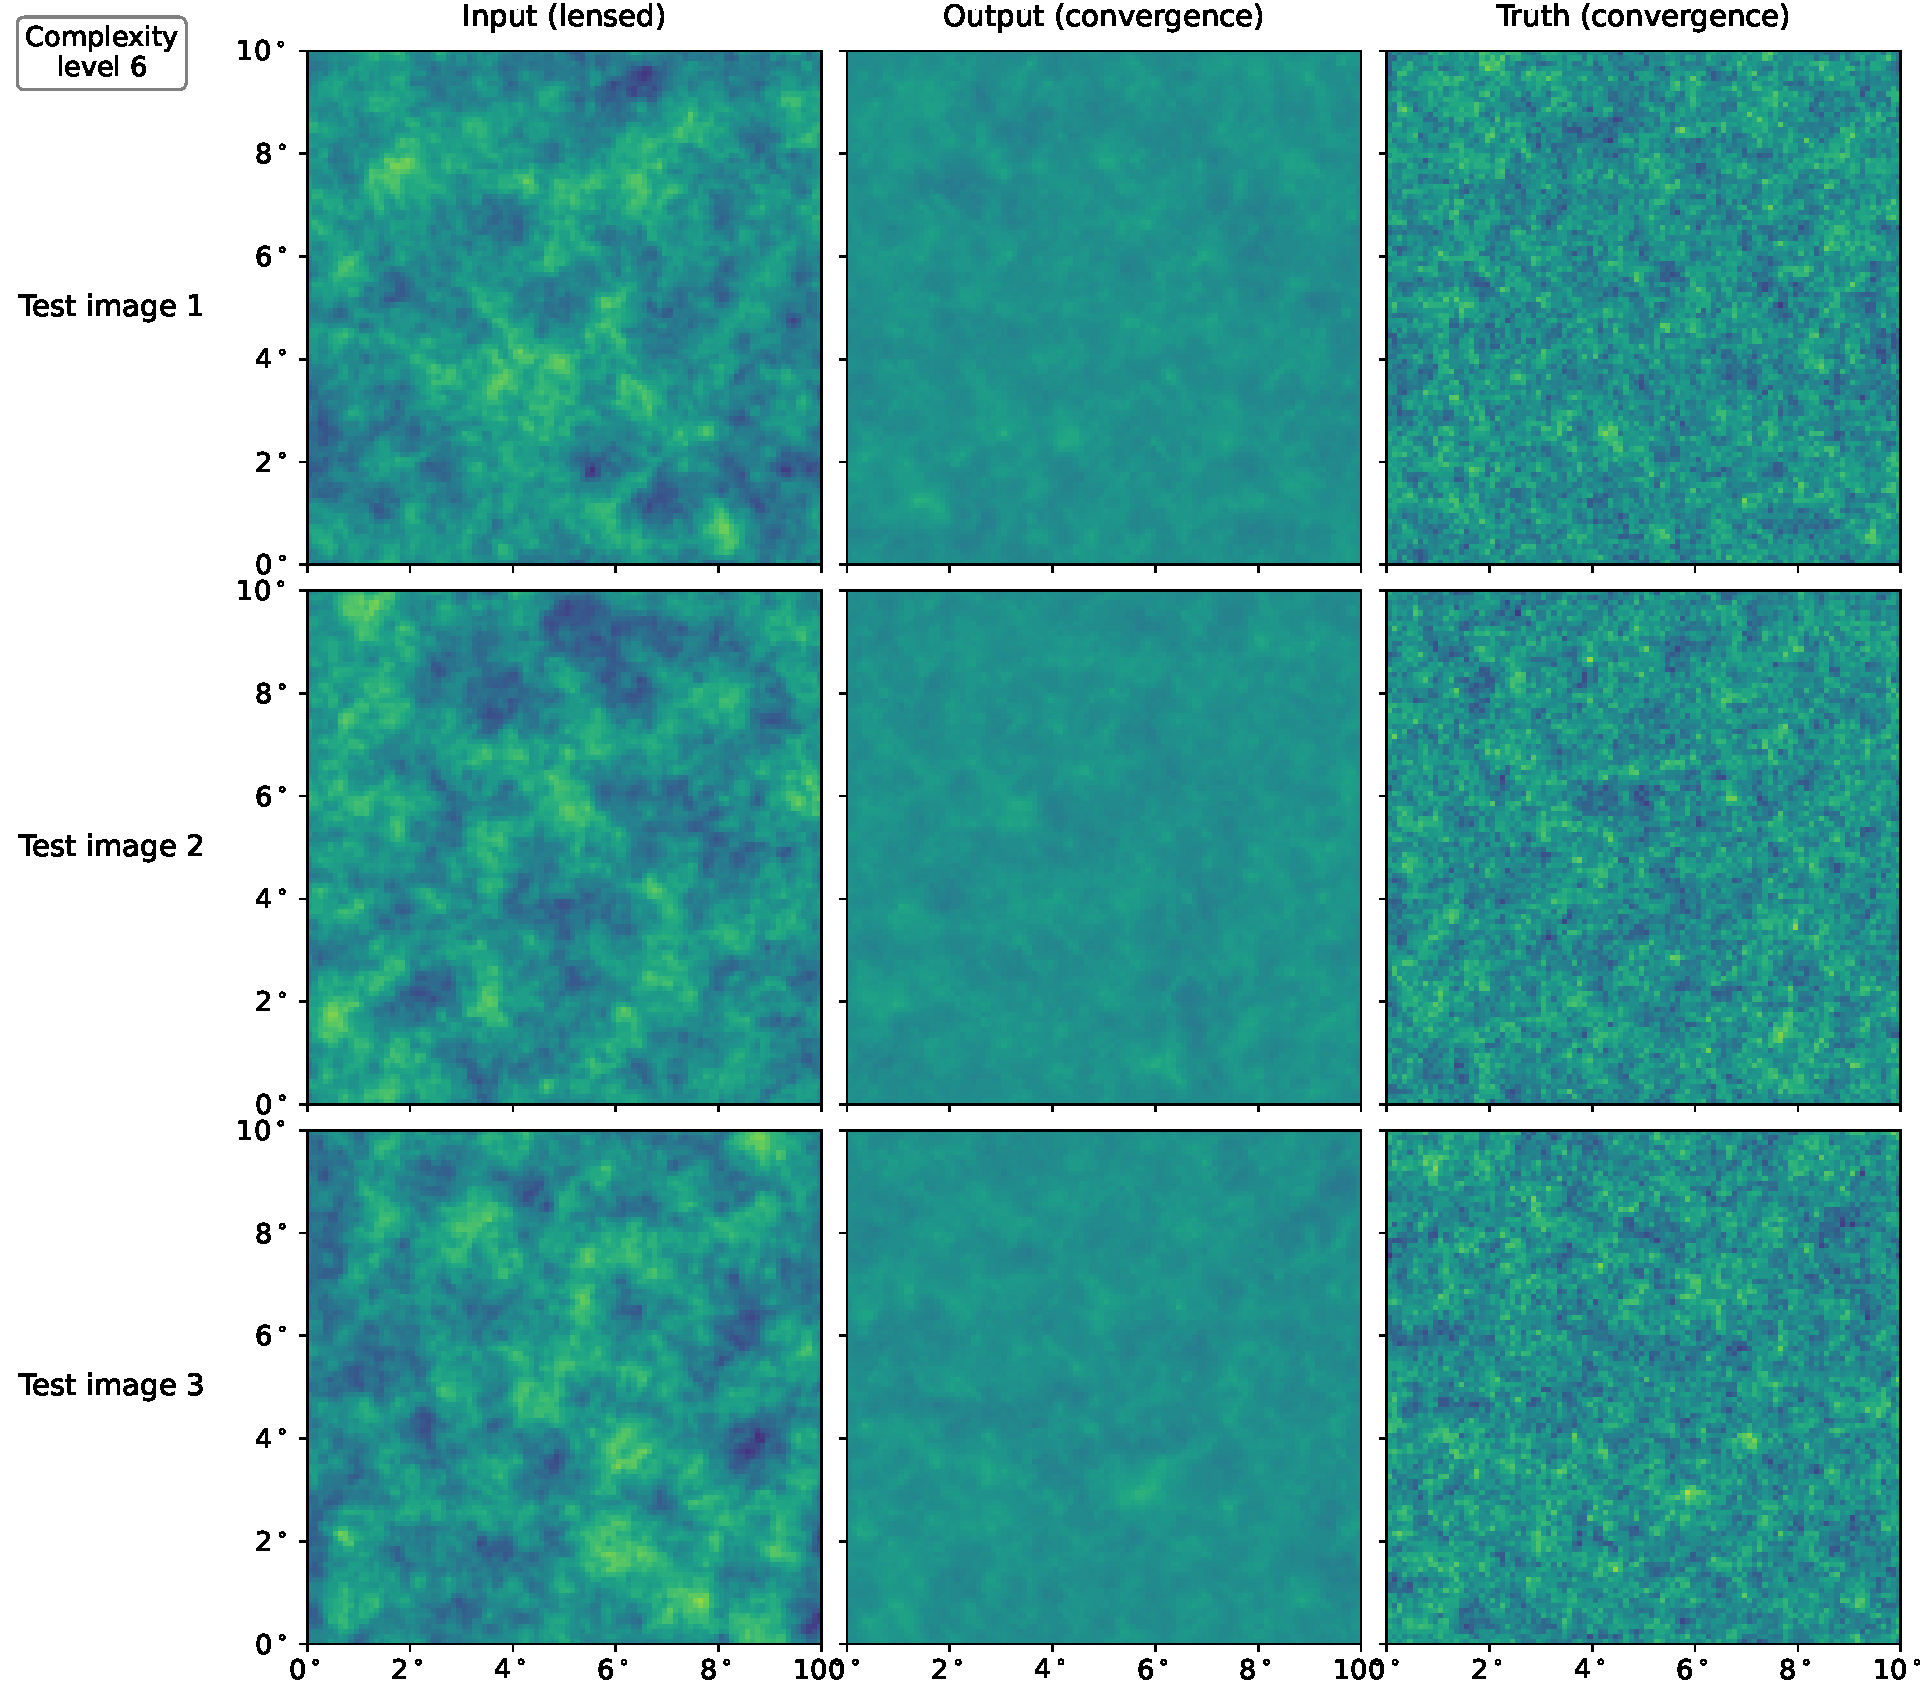
\includegraphics[width=\textwidth]{v6_3x3}
\caption{Performance of the best-performing \texttt{L6\_baseline} model for complexity level 6 (described in \autoref{ml_Sec:v6}) on three previously unseen test images. Rows correspond to the different test images, while the columns show, from left to right: the lensed CMB map given as input to the model, the predicted convergence map produced by the model, and the true convergence map that was used to generate the test image in the first column. The model was trained for 70 epochs on a training set of 9800 samples augmented by a factor 8, with a validation set of 200 samples which was not augmented.}
\label{ml_Fig:v6_3x3}
\end{figure}

After training, each model was assessed using a test set containing 3 previously unseen images. The resulting estimated convergence map is shown for each image along with the corresponding true convergence map in \autoref{ml_Fig:v6_3x3}, for the best-performing \texttt{L6\_baseline} model. It appears that most features are correctly recovered, but with a too-small amplitude. Similar performance was observed for the \texttt{L6\_x2depth}  model, while the \texttt{L6\_x4depth} model did not appear to be able to recover any features in the true convergence maps.

\begin{figure}[tp]
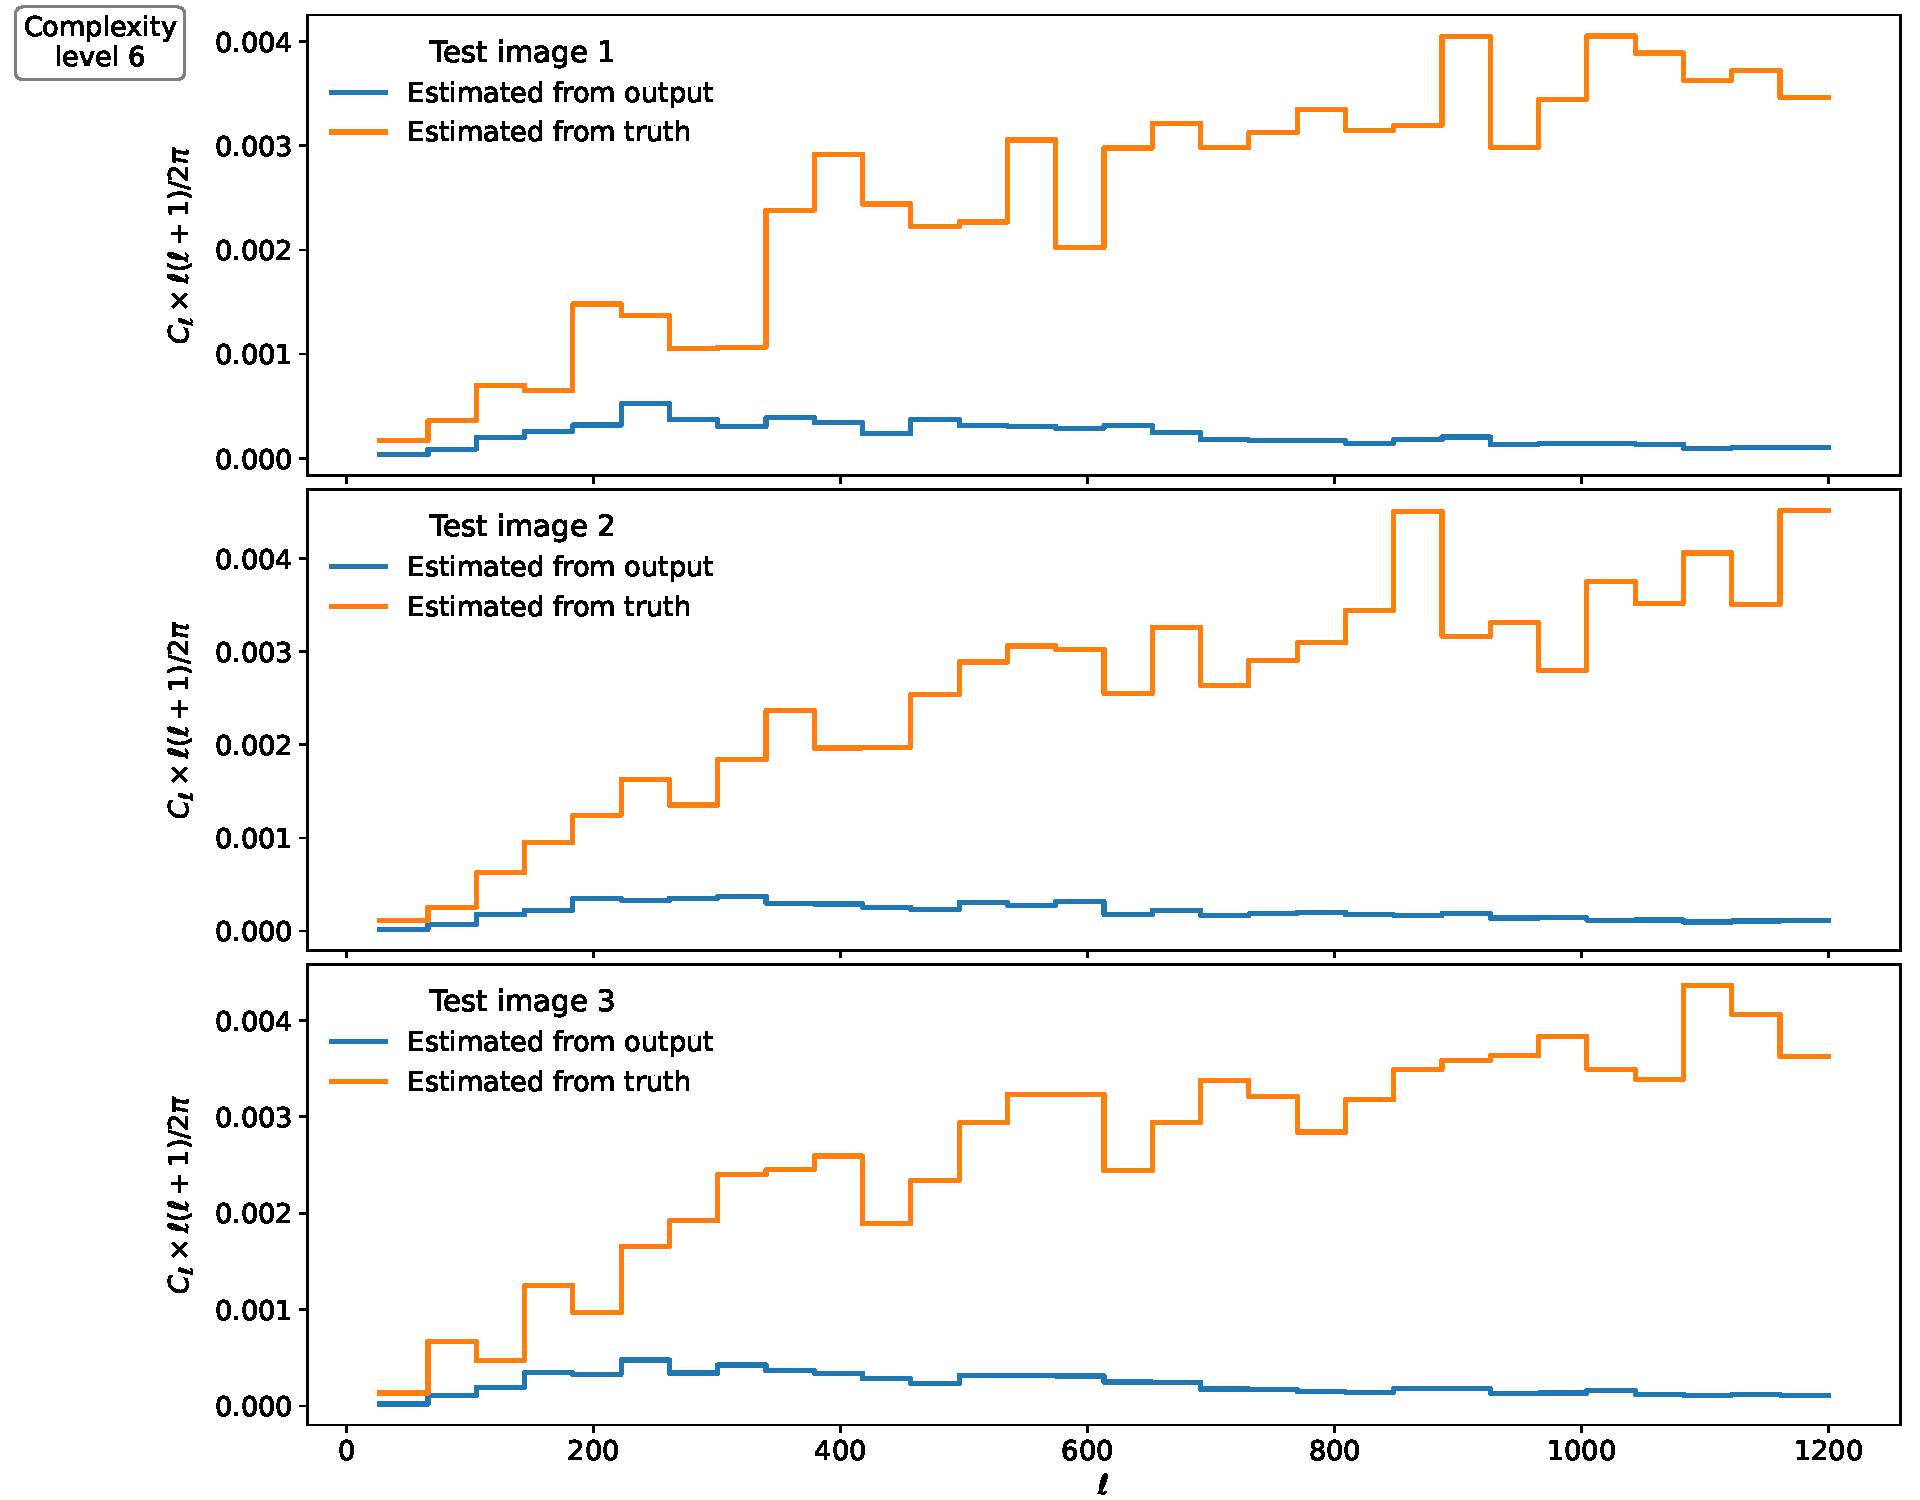
\includegraphics[width=\textwidth]{v6_cls}
\caption{Power spectra estimated from the convergence maps shown in \autoref{ml_Fig:v6_3x3}. Rows correspond to the three different test images. The blue solid line shows the power spectrum estimated from the predicted convergence map output by the convolutional neural network, while the orange dashed line shows the power spectrum estimated from the true convergence map. Results shown are for the \texttt{L5\_baseline} model for complexity level 6 (described in \autoref{ml_Sec:v6}). The model was trained for 70 epochs on a training set of 9800 samples augmented by a factor 8, with a validation set of 200 samples which was not augmented.}
\label{ml_Fig:v6_cls}
\end{figure}

Power spectra were also estimated, and are shown for the \texttt{L6\_baseline} model in \autoref{ml_Fig:v6_cls}. It appears that on larger scales (below $\ell \sim 500$), features are recovered at a reduced amplitude, whereas on smaller scales they are absent entirely, although the reduced amplitude as a function of scale makes a comparison difficult.

This marks the final extent of the project at the time of writing. Possible future directions in which to continue this work are discussed in \autoref{ml_Sec:discussion} below, along with the achievements and challenges of the work to date.

\clearpage
\section{Discussion}
\label{ml_Sec:discussion}

This chapter has presented an initial exploration of the use of convolutional neural networks for the estimation of weak lensing shear. While many issues remain outstanding, and the conditions investigated have been far short of full realism, the method has nonetheless shown promise. With a restricted signal resolution (using $\lmax$ = 50 in the input convergence power spectrum) and an exaggerated lensing effect by a factor 5--30, a convolutional neural network given a lensed CMB map was able to recover the corresponding convergence map to a high degree of accuracy (Figures \ref{ml_Fig:v2_3x3} and \ref{ml_Fig:v3_3x3}). Even with the lensing exaggeration removed, a good degree of recovery was observed (\autoref{ml_Fig:v4_3x3}). However, smaller-scale features in the convergence maps have not been recovered, and their presence seems to have hindered the recovery of the larger-scale features (\autoref{ml_Fig:v6_3x3}).

Besides imperfect performance, there have been a number of other issues. The sudden divergence of training and validation loss during training, seen most prominently in \autoref{ml_Fig:v5_loss}, is not understood. The failure of the \texttt{L5\_deep} model to recover from this divergence is of particular concern. This issue did not arise again, nor could records be found in the literature of similar problems. As mentioned above, it should not be permitted according to the update rules of the Adam optimiser (\autoref{ml_Eqn:theta_update_rule}). Another challenge is that of computational requirements, which rapidly increased as complexity was added. These arise from all steps of the data generation, model building, and training processes. Data generation is time-consuming and large training sets can require a huge volume of storage, which must be accessible to the machine(s) used for training. Training is itself a slow process and the memory requirements for an image-to-image pipeline quickly spiral as resolution and model complexity are increased, which they must be to achieve high levels of both realism and performance. In this work, these requirements at many stages forced a reduction in complexity from what could have otherwise been investigated.

Other than more computing resources, there are many ways in which performance could potentially be improved at the current level of complexity. For example, the learning rate $\alpha$ used in the Adam optimiser (see \autoref{ml_Sec:cnns}) has been held constant throughout this work, and while other values were explored, each was always treated as constant. Variable learning rates hold some potential promise; methods include learning rate schedulers, which vary the learning rate as a function of training epoch, or dynamic methods such as reducing the learning rate upon reaching a loss plateau. Another possibility is integrating the training data generation into the training pipeline for a limitless supply of training data, which need not be stored on disk, thereby circumventing one of the computational restrictions discussed above. This idea has not been tested, but if implemented well could potentially only slow the training process minimally. Its advantage would be to increase the rate and eventual amount of learning, which is naturally reduced each time the training set is repeated.

While remaining within the CMB lensing context, there are many additional layers of complexity that can be added. The main such angle explored here was resolution, which is still far below a realistic combination of a wide field and small pixel size. As wider fields are explored, the flat-sky approximation used here becomes more inaccurate. An extension to curved-sky geometry with appropriate pixelisation such as HEALPix is attractive but challenging, although methods for implementing convolutional neural networks in this context do exist \citep{Perraudin2019}. In addition, a telescope beam and detector noise have been neglected throughout this work, both of which must be added to simulate a realistic case. There is also the problem that a single known cosmology has been used to produce all of the training, validation, and test data. In practice, we cannot know the true cosmology, so it is necessary to take this into consideration in training and testing.

Finally, as described in the introduction to the chapter in \autoref{ml_Sec:intro}, the context in which this work is motivated is not CMB lensing but instead galaxy lensing using radio observations, with an ultimate aim of developing a method to estimate weak lensing shear directly from radio visibilities. It is essential that such methods are developed and refined in advance of the influx of data predicted to arrive from the SKA in the next decade. The work presented in this chapter has not begun to even attempt to face this challenge. It should not be necessary, though, to master CMB lensing before moving onto radio galaxy lensing. It could be argued that the results presented in this chapter show sufficient promise that now is the appropriate time to move onto applying these methods towards the goal of accurate and high-precision weak lensing analyses with the SKA.


% % Uncomment to build alone without subfiles:
% \printbibliography[heading=bibintoc]
% \end{document}
